\chapter{Stokes 方程}\label{chap:stokes}

\begin{note}[动机]\label{note:stokes-motivation}
Stokes 方程(Stokes equations)刻画最简单的不可压缩流问题.这类问题是稳态的,对流项可以忽略,因此得到的模型是线性的.于是,第 2.19 节笔记中提到的那些困难,最终只剩下速度与压力之间的耦合.

分析 Stokes 方程及其有限元离散,已经会用到许多重要技巧;这些技巧也将用于分析更复杂的问题.
\end{note}

\section{连续方程}\label{sec:stokes-continuous-equations}

\begin{note}[Stokes 方程]\label{note:stokes-equations}
考虑定常流动,即 $\partial_t\bm{u}=0$.若流速还很低,也就是 Reynolds 数很小,则黏性项 $-\operatorname{Re}^{-1}\Delta\bm{u}$ 占主导,对流项 $(\bm{u}\cdot\nabla)\bm{u}$ 可以忽略.将所得动量方程乘以 Reynolds 数,并据此重新定义压力和右端项,可得所谓的 Stokes 方程:
\begin{equation}\label{eq:stokes-strong}
\begin{aligned}
  -\Delta\bm{u}+\nabla p&=\bm{f}
       &&\text{于 }\Omega,\\
  \nabla\cdot\bm{u}&=0
       &&\text{于 }\Omega.
\end{aligned}
\end{equation}
该方程组还须配以适当的边界条件.

下面将应用第\hyperref[sec:abstract-saddle-point]{3.1 节}和第\hyperref[sec:continuous-flow-function-spaces]{3.2 节}的理论研究系统\cref{eq:stokes-strong}.为简化表述,本章先考虑齐次 Dirichlet 边界条件 $\bm{u}=\bm{0}$ 于 $\partial\Omega$.
\end{note}

\begin{note}[Stokes 方程的弱形式]\label{note:stokes-weak-form}
对方程乘以检验函数,在 $\Omega$ 上积分,再用分部积分把导数从解转移到检验函数,就得到带齐次 Dirichlet 边界条件的 Stokes 方程弱形式.具体而言,给定 $\bm{f}\in H^{-1}(\Omega)^d$,求
$(\bm{u},p)\in H_0^1(\Omega)^d\times L_0^2(\Omega)$,使得
\begin{equation}\label{eq:stokes-weak}
\begin{aligned}
  (\nabla\bm{u},\nabla\bm{v})
    -(\nabla\cdot\bm{v},p)
    &=\langle\bm{f},\bm{v}\rangle_{H^{-1}(\Omega),H_0^1(\Omega)}
       &&\forall\bm{v}\in H_0^1(\Omega)^d,\\
  -(\nabla\cdot\bm{u},q)&=0
       &&\forall q\in L_0^2(\Omega).
\end{aligned}
\end{equation}
将第 3.1 节所讨论的抽象线性鞍点问题中的空间取为 $V=H_0^1(\Omega)^d$、$Q=L_0^2(\Omega)$,并赋予范数
\[
  \|\bm{v}\|_V=|\bm{v}|_{H^1(\Omega)},
  \qquad \|q\|_Q=\|q\|_{L^2(\Omega)},
\]
再令
\[
  a(\bm{u},\bm{v})=(\nabla\bm{u},\nabla\bm{v}),
  \qquad b(\bm{v},q)=-(\nabla\cdot\bm{v},q),
  \qquad r=0,
\]
则\cref{eq:stokes-weak}的弱形式属于该抽象框架.它还可等价地写为:求 $(\bm{u},p)\in V\times Q$,使得
\begin{equation}\label{eq:stokes-abstract-weak}
  a(\bm{u},\bm{v})+b(\bm{v},p)-b(\bm{u},q)
   =\langle\bm{f},\bm{v}\rangle_{V',V}
   \quad\forall(\bm{v},q)\in V\times Q.
\end{equation}
若\cref{eq:stokes-weak}成立,从第一式减去第二式即可得到\cref{eq:stokes-abstract-weak}.反过来,在\cref{eq:stokes-abstract-weak}中分别取检验函数对 $(\bm{v},0)$ 和 $(\bm{0},q)$,便得到\cref{eq:stokes-weak}的两条方程.

令 $V_0=V_{\mathrm{div}}$,即第\hyperref[sec:continuous-flow-function-spaces]{3.2 节}中定义的弱散度为零函数空间.与\cref{eq:stokes-weak}对应、并对应于抽象问题\cref{eq:reduced-saddle-subspace}的约化问题为:求 $\bm{u}\in V_{\mathrm{div}}$,使得
\begin{equation}\label{eq:stokes-divergence-free-weak}
  (\nabla\bm{u},\nabla\bm{v})
    =\langle\bm{f},\bm{v}\rangle_{V',V}
    \quad\forall\bm{v}\in V_{\mathrm{div}}.
\end{equation}
\end{note}

\begin{note}[黏性项的速度形变率张量形式]\label{note:stokes-deformation-tensor}
构造变分形式时,黏性项也可以从 $-2\nabla\cdot(\bm{D}(\bm{u}))$ 出发;根据\cref{eq:viscous-term-laplacian},它与 $-\Delta\bm{u}$ 等价.将此项与检验函数 $\bm{v}\in V$ 作内积并分部积分;再利用张量的 $L^2(\Omega)$ 内积按分量定义,以及 $\bm{D}(\bm{u})$ 的对称性,可得
\begin{equation}\label{eq:stokes-deformation-tensor-form}
\begin{aligned}
  -2(\nabla\cdot\bm{D}(\bm{u}),\bm{v})
   &=2(\bm{D}(\bm{u}),\nabla\bm{v})\\
   &=(\bm{D}(\bm{u}),\nabla\bm{v})
      +(\bm{D}(\bm{u}),(\nabla\bm{v})^\mathsf{T})\\
   &=(\bm{D}(\bm{u}),\nabla\bm{v})
      +(\bm{D}(\bm{u})^\mathsf{T},(\nabla\bm{v})^\mathsf{T})\\
   &=(\bm{D}(\bm{u}),\nabla\bm{v})
      +(\bm{D}(\bm{u}),(\nabla\bm{v})^\mathsf{T})\\
   &=2(\bm{D}(\bm{u}),\bm{D}(\bm{v})).
\end{aligned}
\end{equation}
\end{note}

\begin{lemma}[双线性型 $a(\cdot,\cdot)$ 的范数]\label{lem:stokes-bilinear-form-norm}
与 Stokes 问题相应的双线性型 $a(\cdot,\cdot)$ 满足 $\|a\|=1$.
\end{lemma}
\begin{proof}
由 Cauchy--Schwarz 不等式\hyperref[eq:appendix-a-10]{(A.10)},
\[
\begin{aligned}
  \|a\|
   &=\sup_{\bm{v},\bm{w}\in V\setminus\{\bm{0}\}}
      \frac{(\nabla\bm{v},\nabla\bm{w})}
      {\|\nabla\bm{v}\|_{L^2(\Omega)}
       \|\nabla\bm{w}\|_{L^2(\Omega)}}\\
   &\leq\sup_{\bm{v},\bm{w}\in V\setminus\{\bm{0}\}}
      \frac{\|\nabla\bm{v}\|_{L^2(\Omega)}
            \|\nabla\bm{w}\|_{L^2(\Omega)}}
      {\|\nabla\bm{v}\|_{L^2(\Omega)}
       \|\nabla\bm{w}\|_{L^2(\Omega)}}=1.
\end{aligned}
\]
取 $\bm{v}=\bm{w}$ 可知该上确界不小于 $1$,故 $\|a\|=1$.
\end{proof}

\begin{theorem}[Stokes 方程解的存在性与唯一性]\label{thm:stokes-4-6}
设 $\Omega\subset\mathbb{R}^d$ 是边界为 Lipschitz 的有界区域,$d\in\{2,3\}$,且 $\bm{f}\in H^{-1}(\Omega)^d$.那么,存在唯一的 $(\bm{u},p)\in H_0^1(\Omega)^d\times L_0^2(\Omega)$,使其满足\cref{eq:stokes-weak}.
\end{theorem}
\begin{proof}
双线性型 $b(\cdot,\cdot)$ 满足 inf-sup 条件,见定理\hyperref[thm:infsup-v-q]{3.46}.此外,双线性型 $a(\cdot,\cdot)$ 关于 $V_{\mathrm{div}}$ 椭圆,因为
\begin{equation}\label{eq:stokes-ellipticity}
  a(\bm{v},\bm{v})
    =|\bm{v}|_{H^1(\Omega)}^2
    =\|\bm{v}\|_V^2
    \quad\forall\bm{v}\in V.
\end{equation}
因此,$a(\cdot,\cdot)$ 在 $V$ 上椭圆,特别也关于 $V_{\mathrm{div}}$ 椭圆;由引理\hyperref[lem:sufficient-condition-ellipticity]{3.19}得到定理结论.
\end{proof}

\begin{lemma}[解的稳定性]\label{lem:stokes-stability}
设定理\hyperref[thm:stokes-4-6]{4.6}的条件成立.那么,Stokes 问题\cref{eq:stokes-weak}的解 $(\bm{u},p)$ 连续依赖于右端项,且
\begin{equation}\label{eq:stokes-velocity-stability}
  \|\bm{u}\|_V=\|\nabla\bm{u}\|_{L^2(\Omega)}
    \leq\|\bm{f}\|_{H^{-1}(\Omega)};
\end{equation}
\begin{equation}\label{eq:stokes-pressure-stability}
  \|p\|_Q=\|p\|_{L^2(\Omega)}
    \leq\frac{2}{\beta_{\mathrm{is}}}
          \|\bm{f}\|_{H^{-1}(\Omega)}.
\end{equation}
若 $\bm{f}\in L^2(\Omega)^d$,则还有
\begin{equation}\label{eq:stokes-helmholtz-stability}
  \|\bm{u}\|_V
    \leq C\|P_{\mathrm{helm}}\bm{f}\|_{L^2(\Omega)},
\end{equation}
其中常数 $C$ 来自 Poincaré 不等式(Poincar\'e inequality)\hyperref[eq:appendix-a-12]{(A.12)}.
\end{lemma}
\index{Poincaré 不等式}
\begin{proof}
在\cref{eq:stokes-divergence-free-weak}中取检验函数 $\bm{v}=\bm{u}$,得到
\[
  (\nabla\bm{u},\nabla\bm{u})
    =\langle\bm{f},\bm{u}\rangle_{V',V}.
\]
由对偶估计,
\[
  \|\nabla\bm{u}\|_{L^2(\Omega)}^2
    \leq\|\bm{f}\|_{H^{-1}(\Omega)}
         \|\nabla\bm{u}\|_{L^2(\Omega)}.
\]
若 $\|\nabla\bm{u}\|_{L^2(\Omega)}=0$,则\cref{eq:stokes-velocity-stability}显然成立;否则,两边除以该范数即得\cref{eq:stokes-velocity-stability}.

估计压力时,使用 inf-sup 条件\cref{eq:infsup-v-q}、方程\cref{eq:stokes-weak}、对偶配对估计及 Cauchy--Schwarz 不等式\hyperref[eq:appendix-a-10]{(A.10)}:
\[
\begin{aligned}
  \|p\|_{L^2(\Omega)}
   &\leq\frac{1}{\beta_{\mathrm{is}}}
       \sup_{\bm{v}\in V\setminus\{\bm{0}\}}
       \frac{-(\nabla\cdot\bm{v},p)}
            {\|\nabla\bm{v}\|_{L^2(\Omega)}}\\
   &=\frac{1}{\beta_{\mathrm{is}}}
       \sup_{\bm{v}\in V\setminus\{\bm{0}\}}
       \frac{\langle\bm{f},\bm{v}\rangle_{V',V}
                    -(\nabla\bm{u},\nabla\bm{v})}
            {\|\nabla\bm{v}\|_{L^2(\Omega)}}\\
   &\leq\frac{1}{\beta_{\mathrm{is}}}
       \sup_{\bm{v}\in V\setminus\{\bm{0}\}}
       \frac{\|\bm{f}\|_{H^{-1}(\Omega)}\|\nabla\bm{v}\|_{L^2(\Omega)}
             +\|\nabla\bm{u}\|_{L^2(\Omega)}
              \|\nabla\bm{v}\|_{L^2(\Omega)}}
            {\|\nabla\bm{v}\|_{L^2(\Omega)}}\\
   &\leq\frac{1}{\beta_{\mathrm{is}}}
       \bigl(\|\bm{f}\|_{H^{-1}(\Omega)}
            +\|\nabla\bm{u}\|_{L^2(\Omega)}\bigr).
\end{aligned}
\]
再代入速度稳定性估计\cref{eq:stokes-velocity-stability},即得\cref{eq:stokes-pressure-stability}.

现设 $\bm{f}\in L^2(\Omega)^d$.由 Helmholtz 分解\cref{eq:helmholtz-decomposition},
\[
  \bm{f}=P_{\mathrm{helm}}\bm{f}+\nabla r,
\]
其中 Helmholtz 投影由定义\hyperref[def:helmholtz-projection]{3.170}给出.分部积分、$\bm{u}\in V_{\mathrm{div}}$、Cauchy--Schwarz 不等式以及 Poincaré 不等式给出
\[
\begin{aligned}
  \|\nabla\bm{u}\|_{L^2(\Omega)}^2
   &=(P_{\mathrm{helm}}\bm{f},\bm{u})
       +(\nabla r,\bm{u})\\
   &=(P_{\mathrm{helm}}\bm{f},\bm{u})\\
   &\leq\|P_{\mathrm{helm}}\bm{f}\|_{L^2(\Omega)}
          \|\bm{u}\|_{L^2(\Omega)}\\
   &\leq C\|P_{\mathrm{helm}}\bm{f}\|_{L^2(\Omega)}
          \|\nabla\bm{u}\|_{L^2(\Omega)}.
\end{aligned}
\]
若 $\|\nabla\bm{u}\|_{L^2(\Omega)}=0$,结论显然成立;否则除以该范数即可得到\cref{eq:stokes-helmholtz-stability}.
\end{proof}

\begin{note}[inf-sup 条件对压力唯一性的作用]\label{note:stokes-pressure-uniqueness}
直接计算可见,inf-sup 条件保证压力的唯一性.齐次 Stokes 方程的弱形式为
\begin{equation}\label{eq:stokes-homogeneous-system}
\begin{aligned}
  a(\bm{u},\bm{v})+b(\bm{v},p)&=0
       &&\forall\bm{v}\in V,\\
  b(\bm{u},q)&=0
       &&\forall q\in Q.
\end{aligned}
\end{equation}
这是一个线性方程组;要证明解唯一,只需证明 $\bm{f}=\bm{0}$ 时必有 $\bm{u}=\bm{0}$ 且 $p=0$.设 $(\bm{u},p)\in V\times Q$ 满足\cref{eq:stokes-homogeneous-system}.取 $(\bm{u},p)$ 为检验函数,得到
\[
  a(\bm{u},\bm{u})+b(\bm{u},p)=0,
  \qquad b(\bm{u},p)=0.
\]
将第二式代入第一式,可得 $a(\bm{u},\bm{u})=0$.由 $a(\cdot,\cdot)$ 关于 $V$ 的椭圆性\cref{eq:stokes-ellipticity},有 $\bm{u}=\bm{0}$.到此为止尚未用到 inf-sup 条件.

在\cref{eq:stokes-homogeneous-system}的第一式中取 $\bm{u}=\bm{0}$,便有
\[
  b(\bm{v},p)=0\quad\forall\bm{v}\in V,
  \qquad\text{从而}\qquad
  \sup_{\bm{v}\in V\setminus\{\bm{0}\}}
       \frac{b(\bm{v},p)}{\|\bm{v}\|_V}=0.
\]
将 inf-sup 条件写成\cref{eq:infsup-pressure-norm-form},并利用 $\beta_{\mathrm{is}}>0$,立即得到 $p=0$(于 $L_0^2(\Omega)$).
\end{note}

\begin{note}[非齐次 Dirichlet 边界条件]\label{note:stokes-nonhomogeneous-dirichlet}
考虑具有边界条件
\[
  \bm{u}=\bm{g}\quad\text{于 }\partial\Omega,
\]
的 Stokes 方程,其中 $\bm{g}\in H^{1/2}(\partial\Omega)^d$,并满足相容条件\cref{eq:dirichlet-flux-compatibility}.

非齐次 Dirichlet 边界条件下 Stokes 方程解的存在性和唯一性,也可由定理\hyperref[thm:stokes-4-6]{4.6}证明.由迹定理(Trace Theorem)定理\hyperref[thm:appendix-a-34]{A.34},存在 $\bm{u}_0\in H^1(\Omega)^d$,使得 $\bm{u}_0=\bm{g}$ 于 $\partial\Omega$.函数 $\bm{u}-\bm{u}_0$ 满足齐次 Dirichlet 边界条件下的 Stokes 方程,只是右端项有所改变.动量方程的新右端仍属于 $H^{-1}(\Omega)^d$,而质量守恒方程的右端则可能是非齐次的.注意,第 3.1 节和第 3.2 节的理论并不要求鞍点问题第二个方程的右端齐次.定理\hyperref[thm:stokes-4-6]{4.6}保证新右端对应的 Stokes 方程存在唯一解;将该解加上 $\bm{u}_0$,便得到原非齐次 Dirichlet 问题的解.

唯一性可用反证法证明:假设存在两个不同的解,则二者之差满足右端为零且边界条件齐次的 Stokes 问题.由定理\hyperref[thm:stokes-4-6]{4.6},该问题的解只能是 $(\bm{0},0)$.因此,不可能存在两个不同的解.
\end{note}

\begin{note}[其他边界条件]\label{note:stokes-other-boundary-conditions}
关于采用 Dirichlet 以外边界条件时 Stokes 问题适定性的研究,可参见\textcite[第 4.1.4 节]{ErnGuermond2004}.
\end{note}

\begin{lemma}[Stokes 问题的 Babuška inf-sup 条件]\label{lem:stokes-babuska-infsup}
在乘积空间上定义范数
\[
  \|(\bm{v},q)\|_*
    :=\|\nabla\bm{v}\|_{L^2(\Omega)}+\|q\|_{L^2(\Omega)}.
\]
并令
\[
  \mathcal{B}((\bm{w},r),(\bm{v},q))
    :=(\nabla\bm{w},\nabla\bm{v})
      -(\nabla\cdot\bm{v},r)
      +(\nabla\cdot\bm{w},q).
\]
则有
\begin{equation}\label{eq:stokes-babuska-infsup}
  \inf_{\substack{(\bm{w},r)\in V\times Q\\
                   (\bm{w},r)\ne(\bm{0},0)}}
   \sup_{\substack{(\bm{v},q)\in V\times Q\\
                    (\bm{v},q)\ne(\bm{0},0)}}
   \frac{\mathcal{B}((\bm{w},r),(\bm{v},q))}
        {\|(\bm{w},r)\|_*\,\|(\bm{v},q)\|_*}
   \geq\beta_{\mathrm{is,Bab}}>0,
\end{equation}
其中
\[
  \frac{1}{\beta_{\mathrm{is,Bab}}}
   =\left(1+\frac{2}{\beta_{\mathrm{is}}}\right)
     +\frac{1}{\beta_{\mathrm{is}}}
        \left(1+\frac{1}{\beta_{\mathrm{is}}}\right).
\]
\end{lemma}
\begin{proof}
任取 $(\bm{w},r)\in V\times Q$.将此对代入 Stokes 方程对应的左端算子,则存在 $(\bm{F},g)\in V'\times Q$,使得
\begin{equation}\label{eq:stokes-babuska-dual-data}
\begin{aligned}
  (\nabla\bm{w},\nabla\bm{v})
     -(\nabla\cdot\bm{v},r)
     &=\langle\bm{F},\bm{v}\rangle_{V',V},\\
  (\nabla\cdot\bm{w},q)&=(g,q)
      \quad\forall(\bm{v},q)\in V\times Q.
\end{aligned}
\end{equation}
令 $\bm{w}_{\mathrm{div}}\in V_{\mathrm{div}}$ 为 $\bm{w}$ 关于 $V$ 内积的正交投影,则 $\bm{w}-\bm{w}_{\mathrm{div}}\in V_{\mathrm{div}}^{\perp}$.由推论\hyperref[cor:each-pressure-is-divergence]{3.44}可知,$\nabla\cdot(\bm{w}-\bm{w}_{\mathrm{div}})\in Q$.结合\cref{eq:stokes-babuska-dual-data}、$\nabla\cdot\bm{w}_{\mathrm{div}}=0$ 及 Cauchy--Schwarz 不等式\hyperref[eq:appendix-a-10]{(A.10)},得到
\[
\begin{aligned}
  (\nabla\cdot\bm{w},\nabla\cdot(\bm{w}-\bm{w}_{\mathrm{div}}))
   &=(\nabla\cdot(\bm{w}-\bm{w}_{\mathrm{div}}),
       \nabla\cdot(\bm{w}-\bm{w}_{\mathrm{div}}))\\
   &=\|\nabla\cdot(\bm{w}-\bm{w}_{\mathrm{div}})\|_{L^2(\Omega)}^2\\
   &=(g,\nabla\cdot(\bm{w}-\bm{w}_{\mathrm{div}}))\\
   &\leq\|g\|_{L^2(\Omega)}
      \|\nabla\cdot(\bm{w}-\bm{w}_{\mathrm{div}})\|_{L^2(\Omega)}.
\end{aligned}
\]
利用这一估计及\cref{eq:infsup-kernel-complement-bound},可得
\[
  \|\nabla(\bm{w}-\bm{w}_{\mathrm{div}})\|_{L^2(\Omega)}
   \leq\frac{1}{\beta_{\mathrm{is}}}
       \|\nabla\cdot(\bm{w}-\bm{w}_{\mathrm{div}})\|_{L^2(\Omega)}
   \leq\frac{1}{\beta_{\mathrm{is}}}\|g\|_{L^2(\Omega)}.
\]

在\cref{eq:stokes-babuska-dual-data}中取 $\bm{v}=\bm{w}_{\mathrm{div}}$,得到
\[
  (\nabla\bm{w},\nabla\bm{w}_{\mathrm{div}})
    -(\nabla\cdot\bm{w}_{\mathrm{div}},r)
   =(\nabla\bm{w},\nabla\bm{w}_{\mathrm{div}})
   =\langle\bm{F},\bm{w}_{\mathrm{div}}\rangle_{V',V}.
\]
由正交性,
\[
\begin{aligned}
  (\nabla\bm{w},\nabla\bm{w}_{\mathrm{div}})
   &=(\nabla(\bm{w}-\bm{w}_{\mathrm{div}}),
         \nabla\bm{w}_{\mathrm{div}})
      +(\nabla\bm{w}_{\mathrm{div}},\nabla\bm{w}_{\mathrm{div}})\\
   &=(\nabla\bm{w}_{\mathrm{div}},
         \nabla\bm{w}_{\mathrm{div}}).
\end{aligned}
\]
利用对偶配对估计可得
\[
  \|\nabla\bm{w}_{\mathrm{div}}\|_{L^2(\Omega)}
     \leq\|\bm{F}\|_{H^{-1}(\Omega)}.
\]
于是由三角不等式,
\begin{equation}\label{eq:stokes-babuska-velocity-bound}
\begin{aligned}
  \|\nabla\bm{w}\|_{L^2(\Omega)}
   &\leq\|\nabla(\bm{w}-\bm{w}_{\mathrm{div}})\|_{L^2(\Omega)}
       +\|\nabla\bm{w}_{\mathrm{div}}\|_{L^2(\Omega)}\\
   &\leq\frac{1}{\beta_{\mathrm{is}}}\|g\|_{L^2(\Omega)}
       +\|\bm{F}\|_{H^{-1}(\Omega)}.
\end{aligned}
\end{equation}
沿用引理\hyperref[lem:stokes-stability]{4.7}中估计压力的同样方法,并结合\cref{eq:stokes-babuska-velocity-bound},可得
\begin{equation}\label{eq:stokes-babuska-pressure-bound}
\begin{aligned}
  \|r\|_{L^2(\Omega)}
   &\leq\frac{1}{\beta_{\mathrm{is}}}
        \left(\|\bm{F}\|_{H^{-1}(\Omega)}
              +\|\nabla\bm{w}\|_{L^2(\Omega)}\right)\\
   &\leq\frac{2}{\beta_{\mathrm{is}}}\|\bm{F}\|_{H^{-1}(\Omega)}
       +\frac{1}{\beta_{\mathrm{is}}^2}\|g\|_{L^2(\Omega)}.
\end{aligned}
\end{equation}

由\cref{eq:stokes-babuska-dual-data},
\[
\begin{aligned}
  \|\bm{F}\|_{H^{-1}(\Omega)}
   &=\sup_{\bm{v}\in V\setminus\{\bm{0}\}}
       \frac{\langle\bm{F},\bm{v}\rangle_{V',V}}
            {\|\nabla\bm{v}\|_{L^2(\Omega)}}\\
   &=\sup_{\bm{v}\in V\setminus\{\bm{0}\}}
       \frac{(\nabla\bm{w},\nabla\bm{v})
                    -(\nabla\cdot\bm{v},r)}
            {\|\nabla\bm{v}\|_{L^2(\Omega)}}.
\end{aligned}
\]
此外,由于 $(\nabla\cdot\bm{w},c)=0$ 对所有常数 $c\in\mathbb{R}$ 成立,
\[
\begin{aligned}
  \|g\|_{L^2(\Omega)}
   &=\sup_{q\in L^2(\Omega)\setminus\{0\}}
       \frac{(g,q)}{\|q\|_{L^2(\Omega)}}
    =\sup_{q\in L^2(\Omega)\setminus\{0\}}
       \frac{(\nabla\cdot\bm{w},q)}{\|q\|_{L^2(\Omega)}}\\
   &=\sup_{q\in Q\setminus\{0\}}
       \frac{(\nabla\cdot\bm{w},q)}{\|q\|_{L^2(\Omega)}}.
\end{aligned}
\]
将\cref{eq:stokes-babuska-velocity-bound}与\cref{eq:stokes-babuska-pressure-bound}相加,并使用如下事实:在联合上确界中取 $q=0$,其值至少不小于只对 $\bm{v}$ 取上确界的值;另一项同理.记
\[
\mathcal{S}(\bm{w},r)
 :=\sup_{(\bm{v},q)\in(V\times Q)\setminus\{(\bm{0},0)\}}
   \frac{(\nabla\bm{w},\nabla\bm{v})
       -(\nabla\cdot\bm{v},r)
       +(\nabla\cdot\bm{w},q)}
        {\|\nabla\bm{v}\|_{L^2(\Omega)}+\|q\|_{L^2(\Omega)}}.
\]
则
\[
\begin{aligned}
  &\|\nabla\bm{w}\|_{L^2(\Omega)}+\|r\|_{L^2(\Omega)}\\
  &\quad\leq
   \left(1+\frac{2}{\beta_{\mathrm{is}}}
       +\frac{1}{\beta_{\mathrm{is}}}
          \left(1+\frac{1}{\beta_{\mathrm{is}}}\right)\right)
       \mathcal{S}(\bm{w},r).
\end{aligned}
\]
由上式给出的 $\beta_{\mathrm{is,Bab}}$ 及 $(\bm{w},r)\in V\times Q$ 的任意性,得到 inf-sup 条件\cref{eq:stokes-babuska-infsup}.
\end{proof}

\begin{note}[动量方程右端各部分的平衡]\label{note:force-on-velocity-pressure}
设 $\bm{f}\in L^2(\Omega)^d$.根据定理\hyperref[thm:helmholtz-decomposition]{3.168},右端项可作 Helmholtz 分解:
\[
  \bm{f}=P_{\mathrm{helm}}\bm{f}+\nabla r,
  \qquad P_{\mathrm{helm}}\bm{f}\in H_{\mathrm{div}}(\Omega),
  \quad \nabla r\in H_{\mathrm{div}}(\Omega)^\perp.
\]
将此分解代入 Stokes 方程的动量平衡\cref{eq:stokes-strong},可得
\begin{equation}\label{eq:stokes-force-helmholtz-strong}
  -\Delta\bm{u}+\nabla p
    =P_{\mathrm{helm}}\bm{f}+\nabla r.
\end{equation}
假设 $\Delta\bm{u},\nabla p\in L^2(\Omega)^d$.此时甚至有 $\Delta\bm{u}\in H_{\mathrm{div}}(\Omega)$.这一点可直接验证:弱导数可以交换,见\textcite[第 5.2.3 节,定理 1]{Evans2010};再利用 $\nabla\cdot\bm{u}=0$,在二维有
\[
\begin{aligned}
  \nabla\cdot\Delta\bm{u}
   &=\partial_x(\partial_{xx}u_1+\partial_{yy}u_1)
       +\partial_y(\partial_{xx}u_2+\partial_{yy}u_2)\\
   &=\partial_{xx}(\partial_xu_1+\partial_yu_2)
       +\partial_{yy}(\partial_xu_1+\partial_yu_2)=0,
\end{aligned}
\]
三维情形同理.

现在考察完整边值问题.在\cref{eq:stokes-weak}的弱形式中代入 $\bm{f}$ 的分解,并假设解足够光滑.分部积分后得到
\begin{equation}\label{eq:stokes-force-helmholtz-weak}
  -(\Delta\bm{u},\bm{v})
    -(\nabla\cdot\bm{v},p)
   =(P_{\mathrm{helm}}\bm{f},\bm{v})
      -(\nabla\cdot\bm{v},r)
      \quad\forall\bm{v}\in V.
\end{equation}
由此可见,无旋力 $\nabla r$ 完全由压力平衡.稳定性估计\cref{eq:stokes-helmholtz-stability}已经表明,无旋力不影响速度.总之,若将 $\bm{f}$ 改为 $\bm{f}+\nabla r$,Stokes 方程的压力解就相应改为 $p+r$.同样,散度为零的力由速度平衡,更确切地说,由 $-\Delta\bm{u}$ 平衡.因此,无旋力与散度为零的力分别由不同变量承担平衡.

\Needspace{4\baselineskip}
推导\cref{eq:stokes-force-helmholtz-weak}时,分部积分所产生的边界积分必须为零.若检验空间为 $V=H_0^1(\Omega)^d$,即 Stokes 方程在整个边界上施加 Dirichlet 条件,就满足这一要求.采用其他边界条件时,特别是含压力项的边界条件(如 do-nothing 条件\cref{eq:do-nothing-condition}),不同类型力对解的影响便不会如此清楚地分离.
\end{note}

\section{有限元误差分析}\label{sec:stokes-finite-element-error-analysis}
\index{有限元误差分析}

\begin{note}[有限元表述]\label{note:stokes-finite-element-formulation}
设 $V^h$ 是速度有限元空间,$Q^h$ 是压力有限元空间.Stokes 方程\cref{eq:stokes-weak}的有限元离散如下:给定 $\bm{f}$,求 $(\bm{u}^h,p^h)\in V^h\times Q^h$,使得
\begin{equation}\label{eq:stokes-fem-problem}
\begin{aligned}
  a^h(\bm{u}^h,\bm{v}^h)
      +b^h(\bm{v}^h,p^h)
   &=\sum_{K\in\mathcal{T}^h}
       \int_K\bm{f}(\bm{x})\cdot\bm{v}^h(\bm{x})\,\mathrm{d}\bm{x}
       &&\forall\bm{v}^h\in V^h,\\
  b^h(\bm{u}^h,q^h)&=0
       &&\forall q^h\in Q^h,
\end{aligned}
\end{equation}
其中
\begin{equation}\label{eq:stokes-fem-bilinear-forms}
\begin{aligned}
  a^h(\bm{v}^h,\bm{w}^h)
    &=\sum_{K\in\mathcal{T}^h}
        (\nabla\bm{v}^h,\nabla\bm{w}^h)_K,\\
  b^h(\bm{v}^h,q^h)
    &=-\sum_{K\in\mathcal{T}^h}
        (\nabla\cdot\bm{v}^h,q^h)_K.
\end{aligned}
\end{equation}
假设右端 $\bm{f}$ 足够光滑,从而\cref{eq:stokes-fem-problem}中动量方程的右端有定义.
\end{note}

\begin{theorem}[有限元 Stokes 方程解的存在性与唯一性]\label{thm:stokes-fem-existence}
设 $\bigl(a^h(\cdot,\cdot)\bigr)^{1/2}$ 在 $V^h$ 上定义一个范数,且离散 inf-sup 条件\cref{eq:discrete-infsup-condition}成立.那么,问题\cref{eq:stokes-fem-problem}存在唯一解.
\end{theorem}
\begin{proof}
若 $\bigl(a^h(\cdot,\cdot)\bigr)^{1/2}$ 是 $V^h$ 上的范数,则双线性型 $a^h(\cdot,\cdot)$ 关于 $V^h$ 椭圆,特别也关于 $V_{\mathrm{div}}^h$ 椭圆.因此,仿照定理\hyperref[thm:stokes-4-6]{4.6}的证明即可得到结论.
\end{proof}

\begin{note}[目标与思路]\label{note:stokes-error-analysis-goal}
有限元误差分析的目标,是在所关注的范数中了解有限元解趋近弱问题解的收敛阶.为此,考虑一族剖分 $\{\mathcal{T}^h\}$ 及其对应的有限元空间族 $\{V^h\times Q^h\}$.导出有限元误差估计的一般步骤如下,例如可参见定理\hyperref[thm:stokes-error-velocity-h1]{4.21}的证明:
\begin{itemize}
  \item 针对所考虑的误差范数,推导一个等式或不等式;
  \item 对该等式或不等式作适当改写,使有限元空间的逼近误差显现出来;
  \item 用若干常数乘以最佳逼近误差,给出所考虑误差范数的上界.
\end{itemize}
第二步通常需要巧妙地加上再减去一些项.最佳逼近误差与具体问题无关,可再用插值误差估计;这类估计属于有限元方法的一般理论,见附录 C.
\end{note}

\subsection{协调且 inf-sup 稳定的有限元空间对}\label{sec:stokes-conforming-stable-pairs}

\begin{note}[协调且 inf-sup 稳定的有限元空间]\label{note:stokes-conforming-stable-spaces}
本节研究协调且 inf-sup 稳定的有限元空间,也就是说,除离散 inf-sup 条件\cref{eq:discrete-infsup-condition}成立外,还有 $V^h\subset V$ 和 $Q^h\subset Q$.相应的双线性型与连续问题中的相同,即 $a^h(\cdot,\cdot)=a(\cdot,\cdot)$、$b^h(\cdot,\cdot)=b(\cdot,\cdot)$.
\end{note}
\index{协调有限元空间}
\index{inf-sup 稳定有限元空间}

\begin{corollary}[有限元问题的唯一可解性]\label{cor:stokes-fem-unique-solvability}
设 $V^h$ 和 $Q^h$ 是协调有限元空间对,且满足离散 inf-sup 条件\cref{eq:discrete-infsup-condition}.那么,有限元问题\cref{eq:stokes-fem-problem}有唯一解.
\end{corollary}
\begin{proof}
根据定理\hyperref[thm:stokes-fem-existence]{4.14},只需证明 $\bigl(a(\cdot,\cdot)\bigr)^{1/2}$ 在 $V^h$ 上定义一个范数.由\cref{eq:stokes-ellipticity},$\bigl(a(\cdot,\cdot)\bigr)^{1/2}$ 在 $V$ 上是范数,因而在 $V$ 的每个子空间 $V^h\subset V$ 上也是范数.
\end{proof}

\begin{lemma}[有限元解的稳定性]\label{lem:stokes-fem-stability}
设 $V^h\times Q^h$ 是 inf-sup 稳定的有限元空间对.那么,问题\cref{eq:stokes-fem-problem}的解满足
\[
\begin{aligned}
  \|\nabla\bm{u}^h\|_{L^2(\Omega)}
    \leq\|\bm{f}\|_{H^{-1}(\Omega)},
  \qquad
  \|p^h\|_{L^2(\Omega)}
    \leq\frac{2}{\beta_{\mathrm{is}}^h}
          \|\bm{f}\|_{H^{-1}(\Omega)}.
\end{aligned}
\]
\end{lemma}
\begin{proof}
证明可仿照引理\hyperref[lem:stokes-stability]{4.7}进行.
\end{proof}

\begin{note}[约化为离散散度为零函数空间上的问题]\label{note:stokes-discrete-divergence-free-reduction}
由线性鞍点问题的抽象理论(第 3.1 节,笔记 3.11)可知,有限元速度近似可通过求解下列问题得到:求 $\bm{u}^h\in V_{\mathrm{div}}^h$,使得
\begin{equation}\label{eq:stokes-discrete-divergence-free-formulation}
  a^h(\bm{u}^h,\bm{v}^h)
    =(\nabla\bm{u}^h,\nabla\bm{v}^h)
    =\langle\bm{f},\bm{v}^h\rangle_{V',V}
    \quad\forall\bm{v}^h\in V_{\mathrm{div}}^h.
\end{equation}
\end{note}

\subsubsection{\texorpdfstring{情形 $V_{\mathrm{div}}^h\not\subset V_{\mathrm{div}}$}{情形 Vdivh 不包含于 Vdiv}}\label{sec:stokes-discrete-divergence-not-subspace}

\begin{note}[情形 $V_{\mathrm{div}}^h\not\subset V_{\mathrm{div}}$]\label{note:stokes-discrete-divergence-not-subspace}
大多数 inf-sup 稳定有限元空间对都属于这种情形.
\end{note}
\index{离散散度为零子空间}

\begin{theorem}[速度梯度 $L^2(\Omega)$ 范数的有限元误差估计]\label{thm:stokes-error-velocity-h1}
设 $\Omega\subset\mathbb{R}^d$($d\in\{2,3\}$)是边界为多面体且为 Lipschitz 连续的有界区域,且 $(\bm{u},p)\in V\times Q$ 是 Stokes 问题\cref{eq:stokes-weak}的唯一解.假设该问题采用协调且 inf-sup 稳定的有限元空间对 $V^h\times Q^h$ 离散,并记 $\bm{u}^h\in V_{\mathrm{div}}^h$ 为离散速度解.那么,有如下误差估计:
\begin{equation}\label{eq:stokes-error-velocity-h1}
\begin{aligned}
  \|\nabla(\bm{u}-\bm{u}^h)\|_{L^2(\Omega)}
   &\leq 2\inf_{\bm{v}^h\in V_{\mathrm{div}}^h}
       \|\nabla(\bm{u}-\bm{v}^h)\|_{L^2(\Omega)}\\
   &\qquad+\inf_{q^h\in Q^h}
       \|p-q^h\|_{L^2(\Omega)}.
\end{aligned}
\end{equation}
\end{theorem}
\begin{proof}
先推导误差方程.由于 $V_{\mathrm{div}}^h\subset V$,可以在连续 Stokes 方程\cref{eq:stokes-abstract-weak}中取 $V_{\mathrm{div}}^h$ 中的函数作检验函数.再利用连续方程的速度解弱散度为零,从连续问题中减去离散问题\cref{eq:stokes-discrete-divergence-free-formulation},得到
\begin{equation}\label{eq:stokes-error-equation}
  (\nabla(\bm{u}-\bm{u}^h),\nabla\bm{v}^h)
      -(\nabla\cdot\bm{v}^h,p)=0
      \quad\forall\bm{v}^h\in V_{\mathrm{div}}^h.
\end{equation}
压力项之所以出现,是因为一般而言 $V_{\mathrm{div}}^h\not\subset V_{\mathrm{div}}$;\cref{eq:stokes-error-equation}即为误差方程.

下面改写压力项,使其中出现压力的逼近误差.由于
\[
  (\nabla\cdot\bm{v}^h,q^h)=0
  \quad\forall q^h\in Q^h,
\]
可得
\begin{equation}\label{eq:stokes-error-equation-pressure-approx}
  (\nabla(\bm{u}-\bm{u}^h),\nabla\bm{v}^h)
     -(\nabla\cdot\bm{v}^h,p-q^h)=0
  \quad\forall\bm{v}^h\in V_{\mathrm{div}}^h,
       \quad\forall q^h\in Q^h.
\end{equation}

接下来引入速度的逼近误差.任取 $\bm{u}$ 在 $V_{\mathrm{div}}^h$ 中的插值函数 $I^h\bm{u}$,将误差分解为
\[
  \bm{u}-\bm{u}^h
   =(\bm{u}-I^h\bm{u})
      -(\bm{u}^h-I^h\bm{u})
   =\eta-\eta^h.
\]
其中 $\eta=\bm{u}-I^h\bm{u}$ 只是有限元空间 $V_{\mathrm{div}}^h$ 的逼近误差,与所研究的方程无关.下面还要用逼近误差估计 $\eta^h$.为此,将上述分解代入\cref{eq:stokes-error-equation-pressure-approx},并取检验函数 $\bm{v}^h=\eta^h$,得到
\begin{equation}\label{eq:stokes-error-eta-identity}
  \|\nabla\eta^h\|_{L^2(\Omega)}^2
   =(\nabla\eta,\nabla\eta^h)
      -(\nabla\cdot\eta^h,p-q^h)
      \quad\forall q^h\in Q^h.
\end{equation}
现在用 Cauchy--Schwarz 不等式\hyperref[eq:appendix-a-10]{(A.10)}估计右端各项:
\[
\left|(\nabla\eta,\nabla\eta^h)\right|
   \leq\|\nabla\eta\|_{L^2(\Omega)}
         \|\nabla\eta^h\|_{L^2(\Omega)},
\]
而结合\cref{eq:divergence-by-gradient-h01},还有
\begin{equation}\label{eq:stokes-error-eta-pressure-bound}
\begin{aligned}
  \left|(\nabla\cdot\eta^h,p-q^h)\right|
   &\leq\|p-q^h\|_{L^2(\Omega)}
          \|\nabla\cdot\eta^h\|_{L^2(\Omega)}\\
   &\leq\|p-q^h\|_{L^2(\Omega)}
          \|\nabla\eta^h\|_{L^2(\Omega)}.
\end{aligned}
\end{equation}
将这两个估计代入\cref{eq:stokes-error-eta-identity},若 $\|\nabla\eta^h\|_{L^2(\Omega)}\ne0$,两边除以该范数,便有
\[
  \|\nabla\eta^h\|_{L^2(\Omega)}
    \leq\|\nabla\eta\|_{L^2(\Omega)}
         +\|p-q^h\|_{L^2(\Omega)}.
\]
若该范数为零,上式显然成立.再由三角不等式,
\[
  \|\nabla(\bm{u}-\bm{u}^h)\|_{L^2(\Omega)}
    \leq2\|\nabla\eta\|_{L^2(\Omega)}
       +\|p-q^h\|_{L^2(\Omega)}.
\]
此估计对任意 $I^h\bm{u}\in V_{\mathrm{div}}^h$ 和任意 $q^h\in Q^h$ 均成立,故得\cref{eq:stokes-error-velocity-h1}.
\end{proof}

\begin{note}[关于误差估计\cref{eq:stokes-error-velocity-h1}]\label{note:stokes-error-velocity-h1}
由\cref{eq:stokes-error-velocity-h1}可知,速度误差在 $V$ 范数中的估计由速度和压力的最佳逼近误差共同控制.出现速度的最佳逼近误差是自然的,因为速度有限元空间必然会影响误差.检查定理\hyperref[thm:stokes-error-velocity-h1]{4.21}的证明可见,压力最佳逼近误差之所以出现,是因为 $V_{\mathrm{div}}^h\not\subset V_{\mathrm{div}}$.否则,\cref{eq:stokes-abstract-weak}左端的第二项会消失,压力也就不会出现在误差估计中.情形 $V_{\mathrm{div}}^h\subset V_{\mathrm{div}}$ 将在第\hyperref[sec:stokes-exactly-divergence-free-pairs]{4.2.1.2 节}进一步讨论.
\end{note}

\begin{note}[区域的条件]\label{note:stokes-error-domain-conditions}
假设区域为多面体,是为了避免三角剖分逼近边界时引入几何误差.要求边界 Lipschitz 连续,则例如是为了保证所考虑区域上的 Sobolev 嵌入成立.具有 Lipschitz 边界的区域在边界附近只位于边界的一侧,见~\textcite[第 67 页]{Adams1975}.在此条件下,二维多边形区域是 Lipschitz 区域;但三维多面体区域并不必然如此.例如,若区域由上下叠放的两个长方体构成,如\cref{fig:stokes-nonlip-polyhedron}所示,那么在一个长方体的棱与另一个长方体的棱相接处,边界就不满足 Lipschitz 条件.详情可参见~\textcite{KralWendland1986,VerchotaVogel2003}.
\end{note}

\begin{elegantfigure}[0.9\linewidth]
\begin{minipage}[c]{0.29\linewidth}
  \captionof{figure}{三维中边界不满足 \mbox{Lipschitz} 连续性的多面体区域(箭头所指的角点处).}
  \label{fig:stokes-nonlip-polyhedron}
\end{minipage}\hfill
\begin{minipage}[c]{0.60\linewidth}
  \includegraphics[page=159,pagebox=cropbox,trim=202.25bp 70.15bp 52.61bp 497.50bp,clip,width=\linewidth]{../input/source/Finite Element Methods for Incompressible Flow Problems.pdf}
\end{minipage}
\end{elegantfigure}

\begin{corollary}[速度散度 $L^2(\Omega)$ 范数的有限元误差估计]\label{cor:stokes-error-divergence}
设定理\hyperref[thm:stokes-error-velocity-h1]{4.21}的假设成立,则
\begin{equation}\label{eq:stokes-error-divergence}
\begin{aligned}
  \|\nabla\cdot\bm{u}^h\|_{L^2(\Omega)}
   &\leq2\inf_{\bm{v}^h\in V_{\mathrm{div}}^h}
       \|\nabla(\bm{u}-\bm{v}^h)\|_{L^2(\Omega)}\\
   &\qquad+\inf_{q^h\in Q^h}
       \|p-q^h\|_{L^2(\Omega)}.
\end{aligned}
\end{equation}
\end{corollary}
\begin{proof}
由 $\nabla\cdot\bm{u}=0$、估计\cref{eq:divergence-by-gradient-h01}以及\cref{eq:stokes-error-velocity-h1},立即得到
\[
  \|\nabla\cdot\bm{u}^h\|_{L^2(\Omega)}
   =\|\nabla\cdot(\bm{u}-\bm{u}^h)\|_{L^2(\Omega)}
   \leq\|\nabla(\bm{u}-\bm{u}^h)\|_{L^2(\Omega)}.
\]
\end{proof}

\begin{theorem}[压力 $L^2(\Omega)$ 范数的有限元误差估计]\label{thm:stokes-error-pressure-l2}
设定理\hyperref[thm:stokes-error-velocity-h1]{4.21}的假设成立.那么,有如下误差估计:
\begin{equation}\label{eq:stokes-error-pressure-l2}
\begin{aligned}
  \|p-p^h\|_{L^2(\Omega)}
   &\leq\frac{2}{\beta_{\mathrm{is}}^h}
      \inf_{\bm{v}^h\in V_{\mathrm{div}}^h}
        \|\nabla(\bm{u}-\bm{v}^h)\|_{L^2(\Omega)}\\
   &\quad+\left(1+\frac{2}{\beta_{\mathrm{is}}^h}\right)
      \inf_{q^h\in Q^h}\|p-q^h\|_{L^2(\Omega)}.
\end{aligned}
\end{equation}
\end{theorem}
\index{压力误差估计}
\begin{proof}
任取 $q^h\in Q^h$.由三角不等式,
\[
  \|p-p^h\|_{L^2(\Omega)}
   \leq\|p-q^h\|_{L^2(\Omega)}
       +\|p^h-q^h\|_{L^2(\Omega)}.
\]
将有限元 Stokes 问题\cref{eq:stokes-fem-problem}中动量方程的右端替换为连续 Stokes 问题\cref{eq:stokes-weak}中动量方程的左端,对任意 $\bm{v}^h\in V^h$ 有
\[
\begin{aligned}
  b(\bm{v}^h,p^h-q^h)
   &=-a(\bm{u}^h,\bm{v}^h)
       +\langle\bm{f},\bm{v}^h\rangle_{V',V}
       -b(\bm{v}^h,q^h)\\
   &=a(\bm{u}-\bm{u}^h,\bm{v}^h)
       +b(\bm{v}^h,p-q^h)
       \quad\forall q^h\in Q^h.
\end{aligned}
\]
由离散 inf-sup 条件\cref{eq:discrete-infsup-condition}、Cauchy--Schwarz 不等式\hyperref[eq:appendix-a-10]{(A.10)}及估计\cref{eq:divergence-by-gradient-h01},可得
\[
\begin{aligned}
  \|p^h-q^h\|_{L^2(\Omega)}
   &\leq\frac{1}{\beta_{\mathrm{is}}^h}
       \sup_{\bm{v}^h\in V^h\setminus\{\bm{0}\}}
       \frac{b(\bm{v}^h,p^h-q^h)}
            {\|\nabla\bm{v}^h\|_{L^2(\Omega)}}\\
   &=\frac{1}{\beta_{\mathrm{is}}^h}
       \sup_{\bm{v}^h\in V^h\setminus\{\bm{0}\}}
       \frac{a(\bm{u}-\bm{u}^h,\bm{v}^h)
            +b(\bm{v}^h,p-q^h)}
            {\|\nabla\bm{v}^h\|_{L^2(\Omega)}}\\
   &\leq\frac{1}{\beta_{\mathrm{is}}^h}
       \left(\|\nabla(\bm{u}-\bm{u}^h)\|_{L^2(\Omega)}
             +\|p-q^h\|_{L^2(\Omega)}\right).
\end{aligned}
\]
再代入速度误差估计\cref{eq:stokes-error-velocity-h1},便得压力误差估计\cref{eq:stokes-error-pressure-l2}.
\end{proof}

\begin{note}[速度误差的 $L^2(\Omega)$ 范数]\label{note:stokes-error-velocity-l2}
利用 Poincaré 不等式\hyperref[eq:appendix-a-12]{(A.12)},可得速度误差在 $L^2(\Omega)$ 范数下的一个简单估计:
\[
  \|\bm{u}-\bm{u}^h\|_{L^2(\Omega)}
     \leq C\|\nabla(\bm{u}-\bm{u}^h)\|_{L^2(\Omega)}.
\]
再结合估计\cref{eq:stokes-error-velocity-h1}即可得到相应误差界.不过,所得估计不是最优的.要推导速度误差 $\|\bm{u}-\bm{u}^h\|_{L^2(\Omega)}$ 的最优估计,还需要额外的假设和分析工具.
\end{note}
\index{斯托克斯方程}

\begin{note}[正则对偶 Stokes 问题]\label{note:stokes-regular-dual-problem}
为了估计速度误差在 $L^2(\Omega)$ 范数下的大小,采用\textcite{Aubin1967,Nitsche1968}的经典方法.为此,需要考虑 Stokes 方程的一个对偶问题(也称伴随问题).对偶算子或伴随算子的构造方法,是在 Stokes 方程的弱形式\hyperref[eq:stokes-weak]{(4.2)}中交换试验函数与解的位置.利用黏性项的对称性并调整各项的顺序,\cref{eq:stokes-weak}左端可写为
\[
  (\nabla\bm{v},\nabla\bm{u})
  +(\nabla\cdot\bm{u},q)
  -(\nabla\cdot\bm{v},p).
\]
接着,以对偶问题的解 $(\phi_{\widehat{\bm{f}}},\xi_{\widehat{\bm{f}}})$ 替换试验函数,并以试验函数替换解 $(\bm{u},p)$,得到对偶问题弱形式的左端:
\[
  (\nabla\phi_{\widehat{\bm{f}}},\nabla\bm{v})
  +(\nabla\cdot\bm{v},\xi_{\widehat{\bm{f}}})
  -(\nabla\cdot\phi_{\widehat{\bm{f}}},q).
\]
分部积分后,对于散度为零的速度空间 $V_{\mathrm{div}}$,对偶 Stokes 问题的强形式如下:给定 $\widehat{\bm{f}}\in L^2(\Omega)$,求 $(\phi_{\widehat{\bm{f}}},\xi_{\widehat{\bm{f}}})\in V\times Q$,使得
\begin{equation}\label{eq:dual-stokes-strong}
\begin{aligned}
  -\Delta\phi_{\widehat{\bm{f}}}
  -\nabla\xi_{\widehat{\bm{f}}}
    &=\widehat{\bm{f}} &&\text{于 }\Omega,\\
  \nabla\cdot\phi_{\widehat{\bm{f}}}
    &=0 &&\text{于 }\Omega.
\end{aligned}
\end{equation}
注意,一般的对偶问题中,散度约束方程的右端也可能非零.

若映射
\begin{equation}\label{eq:dual-stokes-regularity-map}
  (\phi_{\widehat{\bm{f}}},\xi_{\widehat{\bm{f}}})
  \longmapsto
  -\Delta\phi_{\widehat{\bm{f}}}
  -\nabla\xi_{\widehat{\bm{f}}}
\end{equation}
是从 $(H^2(\Omega)\cap V)\times(H^1(\Omega)\cap Q)$ 到 $L^2(\Omega)$ 的同构,就称问题\cref{eq:dual-stokes-strong}是正则的.与 Stokes 方程本身相比,这要求更高的正则性,即 $\phi_{\widehat{\bm{f}}}\in H^2(\Omega)$ 且 $\xi_{\widehat{\bm{f}}}\in H^1(\Omega)$.可以证明,二维和三维中的有界凸多面体区域满足这一正则性条件,参见\textcite{KelloggOsborn1976,Dauge1989}.
\end{note}

\begin{theorem}[速度 $L^2(\Omega)$ 范数的有限元误差估计]\label{thm:stokes-error-velocity-l2}
设定理\hyperref[thm:stokes-error-velocity-h1]{4.21}的假设成立,并设 $(\phi_{\widehat{\bm{f}}},\xi_{\widehat{\bm{f}}})$ 是问题\cref{eq:dual-stokes-strong}的解.那么,速度的 $L^2(\Omega)$ 误差满足如下估计:
\begingroup\small
\begin{equation}\label{eq:stokes-error-velocity-l2}
\begin{aligned}
  \|\bm{u}-\bm{u}^h\|_{L^2(\Omega)}
  &\leq
  \left(
    \|\nabla(\bm{u}-\bm{u}^h)\|_{L^2(\Omega)}
    +\inf_{q^h\in Q^h}\|p-q^h\|_{L^2(\Omega)}
  \right)\\
  &\quad\times
  \sup_{\substack{\widehat{\bm{f}}\in L^2(\Omega)\\
                   \widehat{\bm{f}}\neq\bm{0}}}
  \frac{1}{\|\widehat{\bm{f}}\|_{L^2(\Omega)}}
  \left[
    \begin{aligned}
      &\inf_{\phi^h\in V_{\mathrm{div}}^h}
        \|\nabla(\phi_{\widehat{\bm{f}}}-\phi^h)\|_{L^2(\Omega)}\\
      &\quad+\inf_{r^h\in Q^h}
        \|\xi_{\widehat{\bm{f}}}-r^h\|_{L^2(\Omega)}
    \end{aligned}
  \right].
\end{aligned}
\end{equation}
\endgroup
\end{theorem}
\index{Aubin--Nitsche 方法}
\begin{proof}
根据 $L^2(\Omega)$ 范数的定义,
\begin{equation}\label{eq:stokes-error-velocity-l2-dual-norm}
  \|\bm{u}-\bm{u}^h\|_{L^2(\Omega)}
  =\sup_{\widehat{\bm{f}}\in L^2(\Omega)\setminus\{\bm{0}\}}
    \frac{(\widehat{\bm{f}},\bm{u}-\bm{u}^h)}
         {\|\widehat{\bm{f}}\|_{L^2(\Omega)}}.
\end{equation}
对偶问题\cref{eq:dual-stokes-strong}的弱形式为:求 $(\phi_{\widehat{\bm{f}}},\xi_{\widehat{\bm{f}}})\in V\times Q$,使得
\[
\begin{aligned}
  (\nabla\bm{v},\nabla\phi_{\widehat{\bm{f}}})
   +(\nabla\cdot\bm{v},\xi_{\widehat{\bm{f}}})
    &=(\widehat{\bm{f}},\bm{v})
      &&\forall\bm{v}\in V,\\
  (\nabla\cdot\phi_{\widehat{\bm{f}}},q)
    &=0 &&\forall q\in Q.
\end{aligned}
\]
在此取 $\bm{v}=\bm{u}-\bm{u}^h\in V$,则\cref{eq:stokes-error-velocity-l2-dual-norm}分子中的内积为
\begin{equation}\label{eq:stokes-error-velocity-l2-dual-identity}
  (\widehat{\bm{f}},\bm{u}-\bm{u}^h)
  =(\nabla(\bm{u}-\bm{u}^h),
     \nabla\phi_{\widehat{\bm{f}}})
   +(\nabla\cdot(\bm{u}-\bm{u}^h),
     \xi_{\widehat{\bm{f}}}).
\end{equation}
现在要在此等式中加入适当项,以得到逼近误差.对任意 $\phi^h\in V_{\mathrm{div}}^h\subset V$ 和 $q^h\in Q^h$,利用 Stokes 方程的弱形式\hyperref[eq:stokes-weak]{(4.2)}及混合有限元问题\cref{eq:stokes-fem-problem}(其在离散散度为零速度空间上的约化形式为\cref{eq:stokes-discrete-divergence-free-formulation}),有
\begin{equation}\label{eq:stokes-error-velocity-l2-discrete-identity}
\begin{aligned}
  &(\nabla(\bm{u}-\bm{u}^h),\nabla\phi^h)\\
  &\quad=(\nabla\cdot\phi^h,p)
      +\langle\bm{f},\phi^h\rangle_{V',V}
      -(\nabla\cdot\phi^h,p^h)
      -\langle\bm{f},\phi^h\rangle_{V',V}\\
  &\quad=(\nabla\cdot\phi^h,p)
       =(\nabla\cdot\phi^h,p-q^h)
       \qquad\forall q^h\in Q^h.
\end{aligned}
\end{equation}
此外,对任意 $q^h,r^h\in Q^h$,分别有
\[
  (\nabla\cdot\phi_{\widehat{\bm{f}}},p-q^h)=0,
  \qquad
  (\nabla\cdot(\bm{u}-\bm{u}^h),r^h)=0,
\]
其中第二个等式成立是因为 $Q^h\subset Q$.将这些项代入\cref{eq:stokes-error-velocity-l2-dual-identity},可得
\begin{equation}\label{eq:stokes-error-velocity-l2-approximation-identity}
\begin{aligned}
  (\widehat{\bm{f}},\bm{u}-\bm{u}^h)
  &= (\nabla(\bm{u}-\bm{u}^h),
      \nabla(\phi_{\widehat{\bm{f}}}-\phi^h))\\
  &\quad +(\nabla\cdot(\phi_{\widehat{\bm{f}}}
                    -\phi^h),p-q^h)\\
  &\quad +(\nabla\cdot(\bm{u}-\bm{u}^h),
           \xi_{\widehat{\bm{f}}}-r^h),
\end{aligned}
\end{equation}
对任意 $\phi^h\in V_{\mathrm{div}}^h$ 及 $q^h,r^h\in Q^h$ 均成立.由 Cauchy--Schwarz 不等式\hyperref[eq:appendix-a-10]{(A.10)}和估计\cref{eq:divergence-by-gradient-h01},可得
\begin{equation}\label{eq:stokes-error-velocity-l2-bound}
\begin{aligned}
  &\bigl|(\widehat{\bm{f}},\bm{u}-\bm{u}^h)\bigr|\\
  &\quad\leq
    \|\nabla(\bm{u}-\bm{u}^h)\|_{L^2(\Omega)}
      \|\nabla(\phi_{\widehat{\bm{f}}}
                    -\phi^h)\|_{L^2(\Omega)}\\
  &\qquad+\|p-q^h\|_{L^2(\Omega)}
      \|\nabla(\phi_{\widehat{\bm{f}}}
                    -\phi^h)\|_{L^2(\Omega)}\\
  &\qquad+\|\nabla(\bm{u}-\bm{u}^h)\|_{L^2(\Omega)}
      \|\xi_{\widehat{\bm{f}}}-r^h\|_{L^2(\Omega)}\\
  &\quad\leq
    \left(
      \|\nabla(\bm{u}-\bm{u}^h)\|_{L^2(\Omega)}
      +\|p-q^h\|_{L^2(\Omega)}
    \right)\\
  &\qquad\times
    \left(
      \|\nabla(\phi_{\widehat{\bm{f}}}
                    -\phi^h)\|_{L^2(\Omega)}
      +\|\xi_{\widehat{\bm{f}}}-r^h\|_{L^2(\Omega)}
    \right).
\end{aligned}
\end{equation}
对任意 $\phi^h\in V_{\mathrm{div}}^h$ 和 $q^h,r^h\in Q^h$ 均有此估计.对所有逼近误差取下确界,即得\cref{eq:stokes-error-velocity-l2}.
\end{proof}
\index{有限元误差分析}

\begin{note}[误差估计对离散 inf-sup 常数的依赖]\label{note:stokes-error-infsup-dependency}
对\cref{eq:stokes-error-velocity-h1,eq:stokes-error-divergence,eq:stokes-error-pressure-l2,eq:stokes-error-velocity-l2}中关于 $V_{\mathrm{div}}^h$ 的最佳逼近误差,可应用估计\cref{eq:best-approximation-vdiv-bound}进行控制;这会引入离散 inf-sup 常数倒数 $(\beta_{\mathrm{is}}^h)^{-1}$,因而得到的是最坏情形估计.

对于能够构造保持离散散度的局部插值算子的有限元空间,可用估计\cref{eq:best-approximation-preserving-interpolant}替代估计\cref{eq:best-approximation-vdiv-bound}.\textcite{GiraultScott2003} 研究了这类算子.此时,速度误差估计中的常数取决于局部离散 inf-sup 常数的倒数,参见\cref{note:alternative-best-approximation-vdiv}.与速度误差估计不同,压力误差估计\cref{eq:stokes-error-pressure-l2}中的常数始终依赖于 $(\beta_{\mathrm{is}}^h)^{-1}$.

以上各种情形中,只要局部 inf-sup 常数或 $\beta_{\mathrm{is}}^h$ 依赖于网格宽度 $h$,就不能期待获得最优阶的收敛速度.
\end{note}
\index{离散 inf-sup 常数}
\index{最佳逼近误差}

\begin{corollary}[协调且 inf-sup 稳定有限元空间对的误差估计]\label{cor:stokes-conforming-infsup-estimates}
设 $\Omega\subset\mathbb{R}^d$($d\in\{2,3\}$)是边界为多面体且为 Lipschitz 连续的有界区域,其上有一族正则且准一致的三角剖分 $\{\mathcal{T}^h\}$.设 $(\bm{u},p)$ 是 Stokes 方程\cref{eq:stokes-weak}的解,且
\[
  \bm{u}\in H^{k+1}(\Omega)\cap V,
  \qquad p\in H^k(\Omega)\cap Q.
\]
对于下列 inf-sup 稳定的有限元空间对:
\begin{itemize}
  \item $P_k^{\mathrm{bubble}}/P_k$,其中 $k=1$(MINI 元);
  \item $P_k/P_{k-1}$、$Q_k/Q_{k-1}$,其中 $k\ge2$(Taylor--Hood 元);
  \item $P_2^{\mathrm{bubble}}/P_1^{\mathrm{disc}}$、$P_3^{\mathrm{bubble}}/P_2^{\mathrm{disc}}$、
        $P_2^{\mathrm{BR}}/P_1^{\mathrm{disc}}$、$Q_k/P_{k-1}^{\mathrm{disc}}$,其中 $k\ge2$;
\end{itemize}
有如下误差估计:
\begin{equation}\label{eq:stokes-fem-convergence-h1}
  \|\nabla(\bm{u}-\bm{u}^h)\|_{L^2(\Omega)}
  \leq Ch^k\left(
    \|\bm{u}\|_{H^{k+1}(\Omega)}
    +\|p\|_{H^k(\Omega)}
  \right);
\end{equation}
\begin{equation}\label{eq:stokes-fem-convergence-divergence}
  \|\nabla\cdot\bm{u}^h\|_{L^2(\Omega)}
  \leq Ch^k\left(
    \|\bm{u}\|_{H^{k+1}(\Omega)}
    +\|p\|_{H^k(\Omega)}
  \right);
\end{equation}
\begin{equation}\label{eq:stokes-fem-convergence-pressure}
  \|p-p^h\|_{L^2(\Omega)}
  \leq Ch^k\left(
    \|\bm{u}\|_{H^{k+1}(\Omega)}
    +\|p\|_{H^k(\Omega)}
  \right).
\end{equation}
若对偶 Stokes 问题\cref{eq:dual-stokes-strong}在\cref{note:stokes-regular-dual-problem}的意义下具有正则解 $(\phi_{\widehat{\bm{f}}},\xi_{\widehat{\bm{f}}})$,则还可得到
\begin{equation}\label{eq:stokes-fem-convergence-velocity-l2}
  \|\bm{u}-\bm{u}^h\|_{L^2(\Omega)}
  \leq Ch^{k+1}\left(
    \|\bm{u}\|_{H^{k+1}(\Omega)}
    +\|p\|_{H^k(\Omega)}
  \right).
\end{equation}
常数 $C$ 取决于离散 inf-sup 常数的倒数,或局部 inf-sup 常数的倒数;参见\cref{note:stokes-error-infsup-dependency}.
\end{corollary}
\index{MINI 元}
\index{Taylor--Hood 元}

\begin{proof}
估计\cref{eq:stokes-error-velocity-h1,eq:stokes-error-divergence,eq:stokes-error-pressure-l2,eq:stokes-error-velocity-l2}中的最佳逼近误差可用插值误差估计,因为最佳逼近误差不大于任一插值误差.因此,\hyperref[eq:stokes-fem-convergence-h1]{式 (4.35)}、\hyperref[eq:stokes-fem-convergence-divergence]{(4.36)}和\hyperref[eq:stokes-fem-convergence-pressure]{(4.37)}直接由有限元空间的插值误差估计推出;速度部分可用估计\cref{eq:best-approximation-vdiv-bound}或\cref{eq:best-approximation-preserving-interpolant}.

估计\cref{eq:stokes-fem-convergence-velocity-l2}中额外的 $h$ 次幂,来自在\cref{eq:stokes-error-velocity-l2}的第二个因子中应用速度插值估计\cref{eq:best-approximation-vdiv-bound}或\cref{eq:best-approximation-preserving-interpolant}以及压力插值估计,并利用 $(\phi_{\widehat{\bm{f}}},\xi_{\widehat{\bm{f}}})$ 的正则性:
\begin{equation}\label{eq:dual-stokes-interpolation-estimate}
\begin{aligned}
  &\inf_{\phi^h\in V_{\mathrm{div}}^h}
      \|\nabla(\phi_{\widehat{\bm{f}}}-\phi^h)\|_{L^2(\Omega)}
    +\inf_{r^h\in Q^h}
      \|\xi_{\widehat{\bm{f}}}-r^h\|_{L^2(\Omega)}\\
  &\qquad\leq Ch\left(
      \|\phi_{\widehat{\bm{f}}}\|_{H^2(\Omega)}
      +\|\xi_{\widehat{\bm{f}}}\|_{H^1(\Omega)}
    \right).
\end{aligned}
\end{equation}
由于映射\cref{eq:dual-stokes-regularity-map}是从 $(H^2(\Omega)\cap V)\times(H^1(\Omega)\cap Q)$ 到 $L^2(\Omega)$ 的同构,存在常数 $C$,使得
\begin{equation}\label{eq:dual-stokes-regularity-estimate}
  \|\phi_{\widehat{\bm{f}}}\|_{H^2(\Omega)}
  +\|\xi_{\widehat{\bm{f}}}\|_{H^1(\Omega)}
  \leq C\|\widehat{\bm{f}}\|_{L^2(\Omega)}.
\end{equation}
将估计\cref{eq:dual-stokes-interpolation-estimate,eq:dual-stokes-regularity-estimate}代入\cref{eq:stokes-error-velocity-l2},即得\cref{eq:stokes-fem-convergence-velocity-l2}.
\end{proof}

\begin{elegantfigure}[0.9\linewidth]
\begin{minipage}[c]{0.30\linewidth}
  \captionof{figure}{例题 4.31 的初始网格(层级 0).}
  \label{fig:stokes-example-initial-grids}
\end{minipage}\hfill
\begin{minipage}[c]{0.45\linewidth}
  \includegraphics[page=165,pagebox=cropbox,trim=162.25bp 497.40bp 51.61bp 59.75bp,clip,width=\linewidth]{../input/source/Finite Element Methods for Incompressible Flow Problems.pdf}
\end{minipage}
\end{elegantfigure}

\begin{example}[支持误差估计的解析例题]\label{ex:stokes-error-estimates-analytical-example}\label{ex:stokes-convergence}
通常使用具有已知(预先给定)解的问题来支持形如\cref{eq:stokes-fem-convergence-h1,eq:stokes-fem-convergence-divergence,eq:stokes-fem-convergence-pressure,eq:stokes-fem-convergence-velocity-l2}的误差估计,并在依次加密的一系列网格上测量数值解相对于该解的误差.这里考虑例题\hyperref[ex:appendix-d-3]{D.3},其定义在单位正方形上.数值模拟采用的初始网格(层级 0)如\cref{fig:stokes-example-initial-grids}所示.在这类非结构或扭曲网格上,数值结果不太可能出现超收敛(superconvergence)现象.为减小求积误差的影响,右端项采用高阶求积公式积分.

不同范数下的误差见\cref{fig:stokes-convergence-gradient-errors}、\cref{fig:stokes-convergence-divergence-errors}、\cref{fig:stokes-convergence-pressure-errors}和\cref{fig:stokes-convergence-velocity-errors}\footnotemark.可以看到,在大多数情况下,数值分析预测的收敛阶与数值模拟中的收敛阶一致.总体而言,同阶的不同离散格式具有相近的精度.只有 $P_2^{\mathrm{bubble}}/P_1^{\mathrm{disc}}$ 空间对所得的压力误差(见\cref{fig:stokes-convergence-pressure-errors})显著高于其他速度二阶、压力一阶的离散格式.
\footnotetext{二维图形由 Matplotlib 绘制,参见~\textcite{Hunter2007};网址:\url{http://matplotlib.org}.}
\index{超收敛}

对于 $P_1^{\mathrm{bubble}}/P_1$ 有限元空间对,压力 $L^2(\Omega)$ 误差的收敛阶比理论分析所预测的高 $0.5$.
\end{example}

\begin{note}[不连续压力近似下的局部质量守恒]\label{note:stokes-local-mass-conservation-discontinuous-pressure}
文献中有时以局部质量守恒作为采用不连续压力近似的理由,即有限元解至少在每个网格单元上满足散度为零,或满足局部质量守恒.

考虑由仿射映射单元构成的网格.由于分片常数函数通常是某个不连续压力有限元空间的子空间,由有限元问题\cref{eq:stokes-fem-problem}的第二个方程可得
\begin{elegantfigure}[0.92\linewidth]
  \includegraphics[page=166,pagebox=cropbox,trim=53.00bp 331.65bp 53.11bp 60.50bp,clip,width=0.95\linewidth]{../input/source/Finite Element Methods for Incompressible Flow Problems.pdf}
  \captionof{figure}{例题 4.31 中不同离散格式的速度梯度误差 $\|\nabla(\bm{u}-\bm{u}^h)\|_{L^2(\Omega)}$ 收敛曲线,分别对应不同阶次 $k$.右上图和左下图中,洋红色曲线与绿色曲线重合.}
  \label{fig:stokes-convergence-gradient-errors}
\end{elegantfigure}
\begin{equation}\label{eq:stokes-discrete-local-mass-sum}
\begin{aligned}
  0
  &=\sum_{K\in\mathcal{T}^h}
      \int_K(\nabla\cdot\bm{u}^h)q^h(\bm{x})\,\mathrm{d}\bm{x}\\
  &=\sum_{K\in\mathcal{T}^h}
      q^h|_K\int_K(\nabla\cdot\bm{u}^h)(\bm{x})\,\mathrm{d}\bm{x}.
\end{aligned}
\end{equation}

此式对所有 $q^h\in P_0$ 或 $q^h\in Q_0$ 均成立.

任取网格单元 $K_1$,再取另一个网格单元 $K_2\ne K_1$.令
\[
  q^h(\bm{x})=
  \begin{cases}
    |K_1|^{-1},&\bm{x}\in K_1,\\
    -|K_2|^{-1},&\bm{x}\in K_2,\\
    0,&\text{其他情形}.
  \end{cases}
\]
由于 $q^h$ 的积分为零,故 $q^h\in L_0^2(\Omega)$.将其代入\cref{eq:stokes-discrete-local-mass-sum},得到
\[
  \int_{K_2}\nabla\cdot\bm{u}^h(\bm{x})\,\mathrm{d}\bm{x}
  =\frac{|K_2|}{|K_1|}
    \int_{K_1}\nabla\cdot\bm{u}^h(\bm{x})\,\mathrm{d}\bm{x}
  \qquad\forall K_2\in\mathcal{T}^h.
\]

由上式可得
\begin{elegantfigure}[0.92\linewidth]
  \includegraphics[page=167,pagebox=cropbox,trim=52.50bp 332.65bp 53.36bp 60.75bp,clip,width=0.95\linewidth]{../input/source/Finite Element Methods for Incompressible Flow Problems.pdf}
  \captionof{figure}{例题 4.31 中不同离散格式的速度散度误差 $\|\nabla\cdot\bm{u}^h\|_{L^2(\Omega)}$ 收敛曲线,分别对应不同阶次 $k$.右上图和左下图中,洋红色曲线与绿色曲线重合.}
  \label{fig:stokes-convergence-divergence-errors}
\end{elegantfigure}

\begin{equation}\label{eq:stokes-discrete-global-divergence}
\begin{aligned}
  \int_\Omega\nabla\cdot\bm{u}^h(\bm{x})\,\mathrm{d}\bm{x}
  &=\sum_{K\in\mathcal{T}^h}
      \int_K\nabla\cdot\bm{u}^h(\bm{x})\,\mathrm{d}\bm{x}\\
  &=\sum_{K\in\mathcal{T}^h}\frac{|K|}{|K_1|}
      \int_{K_1}\nabla\cdot\bm{u}^h(\bm{x})\,\mathrm{d}\bm{x}\\
  &=\frac{|\Omega|}{|K_1|}
      \int_{K_1}\nabla\cdot\bm{u}^h(\bm{x})\,\mathrm{d}\bm{x}.
\end{aligned}
\end{equation}

另一方面,由分部积分公式,
\[
  \int_\Omega\nabla\cdot\bm{u}^h(\bm{x})\,\mathrm{d}\bm{x}
  =\int_{\partial\Omega}\bm{u}^h\cdot\bm{n}(\bm{s})\,\mathrm{d}\bm{s}
  =0.
\]
\begin{elegantfigure}[0.92\linewidth]
  \includegraphics[page=168,pagebox=cropbox,trim=52.50bp 334.65bp 53.36bp 60.75bp,clip,width=0.95\linewidth]{../input/source/Finite Element Methods for Incompressible Flow Problems.pdf}
  \captionof{figure}{例题 4.31 中不同离散格式的压力误差 $\|p-p^h\|_{L^2(\Omega)}$ 收敛曲线,分别对应不同阶次 $k$.}
  \label{fig:stokes-convergence-pressure-errors}
\end{elegantfigure}

因此,\cref{eq:stokes-discrete-global-divergence}右端的积分因子为零.由于 $K_1$ 任意,便有局部质量守恒:
\begin{equation}\label{eq:stokes-discrete-local-mass-conservation}
  \int_K\nabla\cdot\bm{u}^h(\bm{x})\,\mathrm{d}\bm{x}=0
  \qquad\forall K\in\mathcal{T}^h.
\end{equation}

然而,从\cref{fig:stokes-convergence-divergence-errors}可以看到,尽管采用不连续压力近似的离散格式满足局部质量守恒\cref{eq:stokes-discrete-local-mass-conservation},其散度误差 $\|\nabla\cdot\bm{u}^h\|_{L^2(\Omega)}$ 的量级与采用连续压力空间的有限元离散格式相同.
\end{note}
\index{局部质量守恒}

\begin{note}[缩放 Stokes 问题]\label{note:stokes-scaled-problem}
有时出于理论研究目的,会考虑如下缩放的 Stokes 问题:
\begin{equation}\label{eq:stokes-scaled-strong}
\begin{aligned}
  -\nu\Delta\bm{u}+\nabla p&=\bm{f} &&\text{于 }\Omega,\\
  \nabla\cdot\bm{u}&=0 &&\text{于 }\Omega,
\end{aligned}
\end{equation}
其中黏性参数 $\nu>0$.这是因为\hyperref[eq:stokes-scaled-strong]{式 (4.44)}中的黏性项与 Navier--Stokes 方程组中的黏性项采用了相同的缩放形式.

\begin{elegantfigure}[0.92\linewidth]
  \includegraphics[page=169,pagebox=cropbox,trim=52.50bp 330.90bp 53.36bp 60.75bp,clip,width=0.95\linewidth]{../input/source/Finite Element Methods for Incompressible Flow Problems.pdf}
  \captionof{figure}{例题 4.31 中不同离散格式的速度误差 $\|\bm{u}-\bm{u}^h\|_{L^2(\Omega)}$ 收敛曲线,分别对应不同阶次 $k$.}
  \label{fig:stokes-convergence-velocity-errors}
\end{elegantfigure}

将动量方程除以 $\nu$,得到
\[
\begin{aligned}
  -\Delta\bm{u}+\nabla\left(\frac{p}{\nu}\right)
    &=\frac{\bm{f}}{\nu} &&\text{于 }\Omega,\\
  \nabla\cdot\bm{u}&=0 &&\text{于 }\Omega.
\end{aligned}
\]
这与未缩放形式\hyperref[eq:stokes-strong]{(4.1)}相同,只是压力和右端项换成了新的量.因此,本节的有限元误差分析仍可照常应用,并得到\cref{eq:stokes-error-velocity-h1,eq:stokes-error-divergence,eq:stokes-error-pressure-l2,eq:stokes-error-velocity-l2}所示类型的估计,其中压力项(以及\cref{eq:stokes-error-velocity-l2}中的对偶压力项)均带有 $\nu^{-1}$ 因子.于是,形如\cref{eq:stokes-fem-convergence-h1,eq:stokes-fem-convergence-divergence}的估计中,$\|p\|_{H^k(\Omega)}$ 前也会出现 $\nu^{-1}$:
\begin{equation}\label{eq:stokes-scaled-error-h1}
\begin{aligned}
  \|\nabla(\bm{u}-\bm{u}^h)\|_{L^2(\Omega)}
  &\leq Ch^k\left(
      \|\bm{u}\|_{H^{k+1}(\Omega)}
      +\nu^{-1}\|p\|_{H^k(\Omega)}
    \right),\\
  \|\nabla\cdot\bm{u}^h\|_{L^2(\Omega)}
  &\leq Ch^k\left(
      \|\bm{u}\|_{H^{k+1}(\Omega)}
      +\nu^{-1}\|p\|_{H^k(\Omega)}
    \right).
\end{aligned}
\end{equation}

估计速度的 $L^2(\Omega)$ 误差时,再次考虑对偶 Stokes 问题\cref{eq:dual-stokes-strong}.由于该问题的黏性系数为 $1$,其解 $\phi_{\widehat{\bm{f}}}$、$\xi_{\widehat{\bm{f}}}$ 以及右端项 $\widehat{\bm{f}}$ 均不依赖于 $\nu$.误差估计的推导与定理\hyperref[thm:stokes-error-velocity-l2]{4.28}的证明相同,只需将式\hyperref[eq:stokes-error-velocity-l2-discrete-identity]{(4.32)}替换为
\[
  (\nabla(\bm{u}-\bm{u}^h),\nabla\phi^h)
  =\frac{1}{\nu}(\nabla\cdot\phi^h,p-q^h)
  \qquad\forall q^h\in Q^h.
\]
于是,式\hyperref[eq:stokes-error-velocity-l2-approximation-identity]{(4.33)}右端的中间项带有 $\nu^{-1}$ 因子,式\hyperref[eq:stokes-error-velocity-l2-bound]{(4.34)}中 $\|p-q^h\|_{L^2(\Omega)}$ 前也随之出现 $\nu^{-1}$.最终得到速度误差估计
\begin{equation}\label{eq:stokes-scaled-error-velocity-l2}
\begin{aligned}
  \|\bm{u}-\bm{u}^h\|_{L^2(\Omega)}
  &\leq Ch^{k+1}\left(
      \|\bm{u}\|_{H^{k+1}(\Omega)}
      +\nu^{-1}\|p\|_{H^k(\Omega)}
    \right)\\
  &\qquad\times\left(
      \|\phi_{\widehat{\bm{f}}}\|_{H^2(\Omega)}
      +\|\xi_{\widehat{\bm{f}}}\|_{H^1(\Omega)}
    \right).
\end{aligned}
\end{equation}
因此,当 $\nu$ 较小时,$\nu^{-1}\|p\|_{H^k(\Omega)}$ 这一项可能主导所有速度误差估计的右端.

压力误差估计\cref{eq:stokes-fem-convergence-pressure}的左端也须乘以 $\nu^{-1}$.对该估计重新缩放后,可得
\begin{equation}\label{eq:stokes-scaled-error-pressure}
  \|p-p^h\|_{L^2(\Omega)}
  \leq Ch^k\left(
    \nu\|\bm{u}\|_{H^{k+1}(\Omega)}
    +\|p\|_{H^k(\Omega)}
  \right).
\end{equation}
\end{note}

\begin{example}[缩放 Stokes 问题]\label{ex:stokes-scaled-example}
再次考虑例题\hyperref[ex:appendix-d-3]{D.3}中的问题;未缩放 Stokes 方程的模拟见\cref{ex:stokes-error-estimates-analytical-example}.由估计\cref{eq:stokes-scaled-error-h1,eq:stokes-scaled-error-velocity-l2}可预期,当 $\nu$ 较小时,速度误差会增大,并按 $\nu^{-1}$ 线性增长.相反,由\cref{eq:stokes-scaled-error-pressure}可预期,当 $\nu$ 较大时,压力误差会增大,并按 $\nu$ 线性增长.

\cref{fig:stokes-example-initial-grids}所示非结构网格上,二阶 Taylor--Hood 有限元空间对 $P_2/P_1$ 的代表性结果见\cref{fig:stokes-scaled-convergence}.速度误差对 $\nu^{-1}$ 的依赖以及压力误差对 $\nu$ 的依赖都很明显.在粗网格上,也能观察到误差分别随 $\nu^{-1}$ 和 $\nu$ 线性变化.不过,误差较大的曲线会以更高的阶下降,直至与不再依赖于 $\nu$ 数值的曲线相交.速度误差的这一下降阶比预期高半阶,压力的 $L^2(\Omega)$ 误差则高一阶.据我们所知,目前尚无对此现象的解释.
\end{example}

\begin{elegantfigure}[0.92\linewidth]
  \includegraphics[page=171,pagebox=cropbox,trim=52.50bp 334.65bp 53.36bp 60.75bp,clip,width=0.95\linewidth]{../input/source/Finite Element Methods for Incompressible Flow Problems.pdf}
  \captionof{figure}{例题 4.34 中缩放 Stokes 问题及 $P_2/P_1$ 有限元空间对的误差收敛曲线.}
  \label{fig:stokes-scaled-convergence}
\end{elegantfigure}


\subsubsection{\texorpdfstring{情形 $V_{\mathrm{div}}^h\subset V_{\mathrm{div}}$}{情形 Vdivh 包含于 Vdiv}}\label{sec:stokes-exactly-divergence-free-pairs}

\begin{note}[满足 $V_{\mathrm{div}}^h\subset V_{\mathrm{div}}$ 的有限元空间对]\label{note:stokes-divergence-free-pairs}
本小节在 $V_{\mathrm{div}}^h\subset V_{\mathrm{div}}$ 的条件下,重新考察第\hyperref[sec:stokes-discrete-divergence-not-subspace]{4.2.1.1 节}中的误差估计证明.此时有若干项消失.一个重要结果是,速度误差估计不再依赖压力有限元空间的最佳逼近误差.此外,\cref{note:stokes-scaled-problem}所讨论的黏性项缩放也不会影响速度误差估计.对于满足 $V_{\mathrm{div}}^h\subset V_{\mathrm{div}}$ 的情形,所得估计更能反映问题的物理特性;$V_{\mathrm{div}}^h\not\subset V_{\mathrm{div}}$ 时的估计则不同,参见\cref{note:force-on-velocity-pressure}.

满足 $V_{\mathrm{div}}^h\subset V_{\mathrm{div}}$ 的协调且 inf-sup 稳定有限元空间对中,最重要的是特殊网格上的 Scott--Vogelius 空间对 $P_k/P_{k-1}^{\mathrm{disc}}$($k\ge d$),见\cref{sec:scott-vogelius}.
\end{note}

\begin{corollary}[满足 $V_{\mathrm{div}}^h\subset V_{\mathrm{div}}$ 的 inf-sup 稳定空间对的速度误差估计]\label{cor:stokes-error-velocity-exactly-divergence-free}
设定理\hyperref[thm:stokes-error-velocity-h1]{4.21}的假设成立,并考虑一个满足 $V_{\mathrm{div}}^h\subset V_{\mathrm{div}}$ 的 inf-sup 稳定有限元空间对.那么,
\begin{equation}\label{eq:stokes-error-velocity-exactly-divergence-free}
  \|\nabla(\bm{u}-\bm{u}^h)\|_{L^2(\Omega)}
  \leq2\inf_{\bm{v}^h\in V_{\mathrm{div}}^h}
      \|\nabla(\bm{u}-\bm{v}^h)\|_{L^2(\Omega)},
\end{equation}
并且
\begin{equation}\label{eq:stokes-discrete-velocity-divergence-zero}
  \|\nabla\cdot\bm{u}^h\|_{L^2(\Omega)}=0.
\end{equation}
\end{corollary}
\begin{proof}
估计\cref{eq:stokes-error-velocity-exactly-divergence-free}的证明与定理\hyperref[thm:stokes-error-velocity-h1]{4.21}相同.对于满足 $V_{\mathrm{div}}^h\subset V_{\mathrm{div}}$ 的空间对,任意 $\phi^h\in V_{\mathrm{div}}^h$ 都有 $\nabla\cdot\phi^h=0$.因此,误差估计证明中式\hyperref[eq:stokes-error-eta-pressure-bound]{(4.24)}所包含的压力项为零.性质\cref{eq:stokes-discrete-velocity-divergence-zero}则直接由 $V_{\mathrm{div}}^h$ 的定义得到.
\end{proof}

\begin{corollary}[满足 $V_{\mathrm{div}}^h\subset V_{\mathrm{div}}$ 的 inf-sup 稳定空间对的速度 $L^2(\Omega)$ 误差估计]\label{cor:stokes-error-velocity-l2-exactly-divergence-free}
设定理\hyperref[thm:stokes-error-velocity-l2]{4.28}的假设成立.若某个 inf-sup 稳定有限元空间对满足 $V_{\mathrm{div}}^h\subset V_{\mathrm{div}}$,则
\begin{equation}\label{eq:stokes-error-velocity-l2-exactly-divergence-free}
\begin{aligned}
  \|\bm{u}-\bm{u}^h\|_{L^2(\Omega)}
  &\leq\|\nabla(\bm{u}-\bm{u}^h)\|_{L^2(\Omega)}\\
  &\quad\times
    \sup_{\substack{\widehat{\bm{f}}\in L^2(\Omega)\\
                     \widehat{\bm{f}}\ne\bm{0}}}
    \frac{1}{\|\widehat{\bm{f}}\|_{L^2(\Omega)}}
    \inf_{\phi^h\in V_{\mathrm{div}}^h}
      \|\nabla(\phi_{\widehat{\bm{f}}}-\phi^h)\|_{L^2(\Omega)}.
\end{aligned}
\end{equation}
\end{corollary}
\begin{proof}
证明过程与定理\hyperref[thm:stokes-error-velocity-l2]{4.28}相同.此外,在式\hyperref[eq:stokes-error-velocity-l2-approximation-identity]{(4.33)}中,还可利用 $\nabla\cdot(\phi^h-\phi_{\widehat{\bm{f}}})=0$ 和 $\nabla\cdot(\bm{u}-\bm{u}^h)=0$ 在弱意义下成立这一事实.
\end{proof}

\begin{note}[满足 $V_{\mathrm{div}}^h\subset V_{\mathrm{div}}$ 的空间对]\label{note:stokes-divergence-free-pair-consequences}
对于满足 $V_{\mathrm{div}}^h\subset V_{\mathrm{div}}$ 的有限元空间对,由估计\cref{eq:stokes-error-velocity-exactly-divergence-free}和性质\cref{eq:stokes-discrete-velocity-divergence-zero}可得
\begin{equation}\label{eq:stokes-exact-divergence-error-h1}
  \|\nabla(\bm{u}-\bm{u}^h)\|_{L^2(\Omega)}
  \leq Ch^k\|\bm{u}\|_{H^{k+1}(\Omega)};
\end{equation}
\begin{equation}\label{eq:stokes-exact-divergence-zero}
  \|\nabla\cdot\bm{u}^h\|_{L^2(\Omega)}=0;
\end{equation}
\begin{equation}\label{eq:stokes-exact-divergence-error-l2}
  \|\bm{u}-\bm{u}^h\|_{L^2(\Omega)}
  \leq Ch^{k+1}\|\bm{u}\|_{H^{k+1}(\Omega)}.
\end{equation}
特别地,这些估计适用于重心加密网格上的 Scott--Vogelius 空间对 $P_k/P_{k-1}^{\mathrm{disc}}$($k\ge d$).
\end{note}
\index{Scott--Vogelius 有限元}

\begin{note}[缩放 Stokes 问题]\label{note:stokes-scaled-divergence-free-pairs}
对于满足 $V_{\mathrm{div}}^h\subset V_{\mathrm{div}}$ 的有限元空间对,考虑缩放 Stokes 问题\cref{eq:stokes-scaled-strong}时,缩放因子 $\nu^{-1}$ 不影响速度误差估计.这与不满足该包含关系的空间对不同,参见\cref{note:stokes-scaled-problem}.
\end{note}

\begin{example}[重心加密网格上零流问题的 Scott--Vogelius 有限元空间对 $P_2/P_1^{\mathrm{disc}}$]\label{ex:stokes-scott-vogelius-no-flow}
本例考虑零流问题(no-flow problem):在区域 $\Omega=(0,1)^2$ 上求解缩放 Stokes 问题\cref{eq:stokes-scaled-strong},预先给定的解为 $\bm{u}=\bm{0}$,压力为
\[
  p(x,y)=10\left((x-0.5)^3y+(1-x)^2(y-0.5)^2-\frac{1}{36}\right).
\]
已知 Scott--Vogelius 空间对在重心加密网格上满足离散 inf-sup 条件,见\cref{sec:scott-vogelius}.网格按如下方式构造:先将单位正方形沿左下角至右上角的对角线剖分为两个三角形,再对该剖分作一次一致加密.随后按\cref{fig:barycentric-refinement}所示进行重心加密,所得网格作为层级 0.完成该网格上的模拟后,去除重心加密,对网格再作一次一致加密,然后重新进行重心加密,得到层级 1.此过程依此继续.

结果见\cref{fig:scott-vogelius-scaled-errors}.速度误差始终为一个较小的常数,与 $\nu$ 的取值无关.

\begin{elegantfigure}[0.92\linewidth]
  \includegraphics[page=173,pagebox=cropbox,trim=52.50bp 93.90bp 53.61bp 297.25bp,clip,width=0.95\linewidth]{../input/source/Finite Element Methods for Incompressible Flow Problems.pdf}
  \captionof{figure}{例题 4.40 中,重心加密网格上的 Scott--Vogelius $P_2/P_1^{\mathrm{disc}}$ 有限元空间对求解缩放 Stokes 问题所得误差的收敛曲线.}
  \label{fig:scott-vogelius-scaled-errors}
\end{elegantfigure}

该常数的增加源于当 $\nu$ 较小时,线性鞍点问题的条件数随之增大.因此,这一增长反映的是求解器中的舍入误差.由于估计\hyperref[eq:stokes-scaled-error-pressure]{(4.47)}右端的第一项为零,预期压力的 $L^2(\Omega)$ 误差与 $\nu$ 无关;数值结果对此显示得很清楚.

作为比较,\cref{fig:stokes-example-initial-grids}所示不规则网格上 Taylor--Hood 有限元 $P_2/P_1$ 的计算结果见\cref{fig:stokes-taylor-hood-scaled-velocity}.

\begin{elegantfigure}[0.92\linewidth]
  \includegraphics[page=174,pagebox=cropbox,trim=52.50bp 469.65bp 53.36bp 60.75bp,clip,width=0.95\linewidth]{../input/source/Finite Element Methods for Incompressible Flow Problems.pdf}
  \captionof{figure}{例题 4.40 中,Taylor--Hood $P_2/P_1$ 有限元空间对求解缩放 Stokes 问题所得速度误差的收敛曲线.}
  \label{fig:stokes-taylor-hood-scaled-velocity}
\end{elegantfigure}

即使 $\nu$ 取中等数值,离散速度场也明显偏离零流场.这个简单算例清楚地展示了速度误差对黏性的依赖,再次说明:当空间对不满足 $V_{\mathrm{div}}^h\subset V_{\mathrm{div}}$ 时,压力可能对速度误差产生显著影响.注意,两组速度误差的收敛阶都比理论分析预测的高 $0.5$ 阶.
\end{example}
\index{Scott--Vogelius 有限元}

\subsection{\texorpdfstring{Stokes 投影(Stokes projection)}{Stokes 投影}}\label{sec:stokes-projection}

\begin{note}[Stokes 投影]\label{note:stokes-projection}
在 Navier--Stokes 方程的有限元误差分析中,有些方法不直接使用 $V_{\mathrm{div}}^h$ 中的最佳逼近误差,而是选取该空间中的一个具体函数,并已知该函数满足所需的插值误差估计;例如,见定理\hyperref[thm:navier-stokes-error-estimate]{7.35}的证明.Stokes 投影便是这类具体函数的一种可能定义.

给定 $(\bm{u},p)\in V_{\mathrm{div}}\times Q$,Stokes 投影 $(I_{\mathrm{St}}^h\bm{u},I_{\mathrm{St}}^hp)\in V_{\mathrm{div}}^h\times Q^h$ 定义为下列问题的解:
\begin{equation}\label{eq:stokes-projection-definition}
\begin{aligned}
  a(I_{\mathrm{St}}^h\bm{u},\bm{v}^h)
  +b(\bm{v}^h,I_{\mathrm{St}}^hp)
  &=a(\bm{u},\bm{v}^h)+b(\bm{v}^h,p)
  &&\forall\bm{v}^h\in V^h,\\
  b(I_{\mathrm{St}}^h\bm{u},q^h)&=0
  &&\forall q^h\in Q^h,
\end{aligned}
\end{equation}
其中 $V^h\times Q^h\subset V\times Q$ 是满足 inf-sup 条件的有限元空间对.
\end{note}
\index{Stokes 投影}

\begin{lemma}[Stokes 投影的稳定性]\label{lem:stokes-projection-stability}
Stokes 投影关于问题解稳定,即
\begin{equation}\label{eq:stokes-projection-stability-velocity}
  \|\nabla I_{\mathrm{St}}^h\bm{u}\|_{L^2(\Omega)}
  \leq \|\nabla\bm{u}\|_{L^2(\Omega)}
       +\|p\|_{L^2(\Omega)},
\end{equation}
\begin{equation}\label{eq:stokes-projection-stability-pressure}
  \|I_{\mathrm{St}}^hp\|_{L^2(\Omega)}
  \leq \frac{2}{\beta_{\mathrm{is}}^h}
       \left(\|\nabla\bm{u}\|_{L^2(\Omega)}
             +\|p\|_{L^2(\Omega)}\right).
\end{equation}
\end{lemma}
\begin{proof}
在 Stokes 投影的定义中选取投影本身作为检验函数,随后照引理\hyperref[lem:stokes-stability]{4.7}的证明进行即可.
\end{proof}

\begin{lemma}[Stokes 投影的逼近性质]\label{lem:stokes-projection-approximation}
设 $\Omega\subset\mathbb{R}^d$($d\in\{2,3\}$)是有界多面体区域,边界为 Lipschitz 连续,且 $(\bm{u},p)\in V\times Q$.假设问题\hyperref[eq:stokes-projection-definition]{(4.54)}采用满足 inf-sup 条件的协调有限元空间 $V^h\times Q^h$ 离散,则
\begin{equation}\label{eq:stokes-projection-best-approximation-velocity}
\begin{aligned}
  \|\nabla(\bm{u}-I_{\mathrm{St}}^h\bm{u})\|_{L^2(\Omega)}
  &\leq 2\left(1+\frac{1}{\beta_{\mathrm{is}}^h}\right)
      \inf_{\bm{v}^h\in V^h}
      \|\nabla(\bm{u}-\bm{v}^h)\|_{L^2(\Omega)}\\
  &\quad+\inf_{q^h\in Q^h}\|p-q^h\|_{L^2(\Omega)},
\end{aligned}
\end{equation}
以及
\begin{equation}\label{eq:stokes-projection-best-approximation-pressure}
\begin{aligned}
  \|p-I_{\mathrm{St}}^hp\|_{L^2(\Omega)}
  &\leq \frac{2}{\beta_{\mathrm{is}}^h}
       \Biggl[\left(1+\frac{1}{\beta_{\mathrm{is}}^h}\right)
       \inf_{\bm{v}^h\in V^h}
       \|\nabla(\bm{u}-\bm{v}^h)\|_{L^2(\Omega)}\\
  &\qquad\quad+\inf_{q^h\in Q^h}\|p-q^h\|_{L^2(\Omega)}\Biggr].
\end{aligned}
\end{equation}
\end{lemma}
\begin{proof}
将问题\hyperref[eq:stokes-projection-definition]{(4.54)}约化到离散散度为零子空间,可得与估计\hyperref[eq:stokes-error-velocity-h1]{(4.21)}相同的结论,只需将 $\bm{u}^h$ 换为 $I_{\mathrm{St}}^h\bm{u}$.随后,速度估计的证明与定理\hyperref[thm:stokes-error-velocity-h1]{4.21}相同;压力逼近估计的证明则沿用定理\hyperref[thm:stokes-error-pressure-l2]{4.25}的论证.两处最后都使用了 $V_{\mathrm{div}}^h$ 的最佳逼近误差估计\cref{eq:best-approximation-vdiv-bound}.
\end{proof}

\begin{note}[Stokes 投影的时间导数与时间导数的 Stokes 投影]\label{note:stokes-projection-time-derivative}
设 $(\bm{u},p)$ 是关于时间足够光滑的函数.若在 Stokes 投影问题\cref{eq:stokes-projection-definition}中以 $(\partial_t\bm{u},\partial_t p)$ 作为右端数据,所得投影为 $(I_{\mathrm{St}}^h\partial_t\bm{u},I_{\mathrm{St}}^h\partial_t p)$.对 Stokes 投影的定义关于时间求导,并交换时间微分与空间积分、空间微分的次序,可得
\[
\begin{aligned}
  &a(\partial_t I_{\mathrm{St}}^h\bm{u},\bm{v}^h)
   +b(\bm{v}^h,\partial_t I_{\mathrm{St}}^hp)\\
  &-b(\partial_t I_{\mathrm{St}}^h\bm{u},q^h)
   =a(\partial_t\bm{u},\bm{v}^h)
    +b(\bm{v}^h,\partial_t p).
\end{aligned}
\] 
因此,$(\partial_t I_{\mathrm{St}}^h\bm{u},\partial_t I_{\mathrm{St}}^hp)\in V^h\times Q^h$ 也是以 $(\partial_t\bm{u},\partial_t p)$ 为右端数据的 Stokes 投影.由于 Stokes 投影唯一,便有
\[
  I_{\mathrm{St}}^h\partial_t\bm{u}
  =\partial_t I_{\mathrm{St}}^h\bm{u},
  \qquad
  I_{\mathrm{St}}^h\partial_t p
  =\partial_t I_{\mathrm{St}}^hp.
\]
这种空间投影与时间微分的可交换性,源于 Stokes 投影定义中的所有项都关于时间呈线性;同理也可推广到更高阶的时间导数.
\end{note}
\index{Stokes 投影!时间导数}

\subsection{最低阶非协调 inf-sup 稳定有限元空间对}\label{sec:stokes-lowest-order-nonconforming-pairs}

\begin{note}[最低阶非协调 inf-sup 稳定有限元空间对]\label{note:stokes-lowest-order-nonconforming-pairs}
最低阶非协调有限元空间对包括:单纯形网格上的 Crouzeix--Raviart 有限元 $P_1^{\mathrm{nc}}/P_0$,以及四边形和六面体网格上的 Rannacher--Turek 元 $Q_1^{\mathrm{rot}}/Q_0$,见第\hyperref[sec:lowest-order-nonconforming]{3.6.5 节}.它们无疑是不可压缩流数值模拟中最常用的非协调有限元空间对.其离散 inf-sup 条件\cref{eq:discrete-infsup-condition}已在第\hyperref[sec:lowest-order-nonconforming]{3.6.5 节}证明或讨论.

本节以 $P_1^{\mathrm{nc}}/P_0$ 空间对为例介绍有限元误差分析.由于 $V^h\not\subset V$,连续空间 $V$ 的性质不能直接传递到 $V^h$,这给分析带来若干技术困难.特别是,必须估计 $V^h$ 不包含于 $V$ 所造成的量,也就是所谓的一致性误差(consistency error).证明会用到协调分片线性有限元空间 $P_1$ 是 $P_1^{\mathrm{nc}}$ 的子空间这一事实.
\end{note}
\index{Crouzeix--Raviart 有限元}
\index{Rannacher--Turek 元}

\begin{note}[有限元问题]\label{note:stokes-nonconforming-fem-problem}
由于非协调离散化中 $V^h\not\subset V$,Stokes 有限元问题必须采用逐网格单元定义的双线性型.给定 $\bm{f}\in L^2(\Omega)^d$,求 $(\bm{u}^h,p^h)\in V^h\times Q^h=P_1^{\mathrm{nc}}\times P_0$,使得
\begin{equation}\label{eq:stokes-nonconforming-fem-problem}
\begin{aligned}
  a^h(\bm{u}^h,\bm{v}^h)+b^h(\bm{v}^h,p^h)
  &=(\bm{f},\bm{v}^h)
  &&\forall\bm{v}^h\in V^h,\\
  b^h(\bm{u}^h,q^h)&=0
  &&\forall q^h\in Q^h,
\end{aligned}
\end{equation}
其中双线性型 $a^h(\cdot,\cdot)$、$b^h(\cdot,\cdot)$ 按\cref{eq:stokes-fem-bilinear-forms}定义.
\end{note}

\begin{corollary}[有限元问题的唯一可解性]\label{cor:stokes-nonconforming-unique-solvability}
有限元问题\cref{eq:stokes-nonconforming-fem-problem}存在唯一解 $(\bm{u}^h,p^h)\in V^h\times Q^h$.
\end{corollary}
\begin{proof}
由定理\hyperref[thm:crouzeix-raviart-infsup]{3.151}可知这些空间对满足离散 inf-sup 条件\cref{eq:discrete-infsup-condition}.根据定理\hyperref[thm:stokes-fem-existence]{4.14},只需证明 $\bigl(a^h(\cdot,\cdot)\bigr)^{1/2}$ 在 $V^h$ 上定义一个范数.该性质已由引理\hyperref[lem:nonconforming-energy-norm]{3.150}证明.
\end{proof}

\begin{note}[约化到离散散度为零函数空间]\label{note:stokes-nonconforming-divergence-free-reduction}
与协调有限元方法相同,误差分析从将鞍点问题\cref{eq:stokes-nonconforming-fem-problem}约化为离散散度为零空间 $V_{\mathrm{div}}^h$ 上的标量问题开始:求 $\bm{u}^h\in V_{\mathrm{div}}^h$,使得
\begin{equation}\label{eq:stokes-nonconforming-divergence-free-problem}
  a^h(\bm{u}^h,\bm{v}^h)
  =(\bm{f},\bm{v}^h)
  \qquad\forall\bm{v}^h\in V_{\mathrm{div}}^h.
\end{equation}
求解问题\cref{eq:stokes-nonconforming-fem-problem}或\cref{eq:stokes-nonconforming-divergence-free-problem},所得有限元速度解相同.
\end{note}

\begin{note}[Poincaré 不等式]\label{note:stokes-nonconforming-poincare}
对 $P_1^{\mathrm{nc}}$ 中的函数 $\bm{v}^h$,在正则三角剖分族上有 Poincaré 不等式(或 Poincaré--Friedrichs 不等式)
\begin{equation}\label{eq:stokes-nonconforming-poincare}
  \|\bm{v}^h\|_{L^2(\Omega)}
  \leq C\|\bm{v}^h\|_{V^h},
\end{equation}
其中
\[
  \|\bm{v}^h\|_{V^h}
  :=\bigl(a^h(\bm{v}^h,\bm{v}^h)\bigr)^{1/2}
  =\left(\sum_{K\in\mathcal{T}^h}
       \|\nabla\bm{v}^h\|_{L^2(K)}^2\right)^{1/2}.
\]
例如,见\textcite{Knobloch2001,Brenner2003}.
\end{note}
\index{Poincaré 不等式}

\begin{lemma}[有限元解的稳定性]\label{lem:stokes-nonconforming-stability}
设 $\bm{f}\in L^2(\Omega)^d$,则问题\cref{eq:stokes-nonconforming-fem-problem}的解满足
\[
\begin{aligned}
  \|\bm{u}^h\|_{V^h}
  &\leq C\|\bm{f}\|_{L^2(\Omega)},\\
  \|p^h\|_{L^2(\Omega)}
  &\leq \frac{2C}{\beta_{\mathrm{is}}^h}
         \|\bm{f}\|_{L^2(\Omega)},
\end{aligned}
\]
其中 $C$ 是 Poincaré 不等式\hyperref[eq:stokes-nonconforming-poincare]{(4.61)}中的常数.
\end{lemma}
\begin{proof}
在问题\cref{eq:stokes-nonconforming-fem-problem}中取有限元解本身作为检验函数,并应用 Cauchy--Schwarz 不等式\hyperref[eq:appendix-a-10]{(A.10)}、Poincaré 不等式\hyperref[eq:stokes-nonconforming-poincare]{(4.61)}和 Young 不等式\hyperref[eq:appendix-a-5]{(A.5)},可得
\[
\begin{aligned}
  \|\bm{u}^h\|_{V^h}^2
  &=a^h(\bm{u}^h,\bm{u}^h)
    =(\bm{f},\bm{u}^h)\\
  &\leq\|\bm{f}\|_{L^2(\Omega)}
        \|\bm{u}^h\|_{L^2(\Omega)}
   \leq C\|\bm{f}\|_{L^2(\Omega)}
        \|\bm{u}^h\|_{V^h},
\end{aligned}
\]
从而得到速度估计.压力估计由离散 inf-sup 条件、有限元方程\cref{eq:stokes-nonconforming-fem-problem}、Cauchy--Schwarz 不等式、Poincaré 不等式以及刚得到的速度稳定性估计给出:
\[
\begin{aligned}
  \|p^h\|_{L^2(\Omega)}
  &\leq\frac{1}{\beta_{\mathrm{is}}^h}
    \sup_{\bm{v}^h\in V^h,\ \bm{v}^h\ne\bm{0}}
    \frac{b^h(\bm{v}^h,p^h)}{\|\bm{v}^h\|_{V^h}}\\
  &=\frac{1}{\beta_{\mathrm{is}}^h}
    \sup_{\bm{v}^h\in V^h,\ \bm{v}^h\ne\bm{0}}
    \frac{(\bm{f},\bm{v}^h)-a^h(\bm{u}^h,\bm{v}^h)}
         {\|\bm{v}^h\|_{V^h}}\\
  &\leq\frac{1}{\beta_{\mathrm{is}}^h}
       \left(C\|\bm{f}\|_{L^2(\Omega)}
             +\|\bm{u}^h\|_{V^h}\right)
   \leq\frac{2C}{\beta_{\mathrm{is}}^h}
       \|\bm{f}\|_{L^2(\Omega)}.
\end{aligned}
\]
\end{proof}

\begin{lemma}[Strang 第二引理:抽象误差估计]\label{lem:stokes-strang-second}
抽象误差估计(abstract error estimate)的 Strang 第二引理(second lemma of Strang)如下.设 $\bm{u}\in V$ 是问题\hyperref[eq:stokes-weak]{(4.4)}的解,$\bm{u}^h\in V^h$ 是问题\hyperref[eq:stokes-nonconforming-divergence-free-problem]{(4.60)}的解,则有误差估计
\begin{equation}\label{eq:stokes-strang-second}
\begin{aligned}
  \|\bm{u}-\bm{u}^h\|_{V^h}
  &\leq 2\inf_{\bm{v}^h\in V_{\mathrm{div}}^h}
        \|\bm{u}-\bm{v}^h\|_{V^h}\\
  &\quad+
    \sup_{\substack{\bm{v}^h\in V_{\mathrm{div}}^h\\
                     \|\bm{v}^h\|_{V^h}=1}}
    \left|a^h(\bm{u},\bm{v}^h)
          -(\bm{f},\bm{v}^h)\right|.
\end{aligned}
\end{equation}
\end{lemma}
\begin{proof}
任取 $\bm{v}^h\in V_{\mathrm{div}}^h$,并作分解
\[
  \bm{u}-\bm{u}^h
  =\bm{u}-\bm{v}^h-(\bm{u}^h-\bm{v}^h)
  =\bm{u}-\bm{v}^h-\symbf{\phi}^h,
\]
其中 $\symbf{\phi}^h:=\bm{u}^h-\bm{v}^h\in V_{\mathrm{div}}^h$.利用问题\hyperref[eq:stokes-nonconforming-divergence-free-problem]{(4.60)}和 Cauchy--Schwarz 不等式,有
\[
\begin{aligned}
  \|\symbf{\phi}^h\|_{V^h}^2
  &=a^h(\symbf{\phi}^h,\symbf{\phi}^h)
    =a^h(\bm{u}^h-\bm{v}^h,\symbf{\phi}^h)\\
  &=a^h(\bm{u}-\bm{v}^h,\symbf{\phi}^h)
    +a^h(\bm{u}^h,\symbf{\phi}^h)
    -a^h(\bm{u},\symbf{\phi}^h)\\
  &=a^h(\bm{u}-\bm{v}^h,\symbf{\phi}^h)
    +(\bm{f},\symbf{\phi}^h)
    -a^h(\bm{u},\symbf{\phi}^h)\\
  &\leq\|\bm{u}-\bm{v}^h\|_{V^h}
        \|\symbf{\phi}^h\|_{V^h}
    +\left|(\bm{f},\symbf{\phi}^h)
            -a^h(\bm{u},\symbf{\phi}^h)\right|.
\end{aligned}
\]
若 $\|\symbf{\phi}^h\|_{V^h}\ne0$,将上式除以该范数;再利用三角不等式
\[
  \|\bm{u}-\bm{u}^h\|_{V^h}
  \leq\|\bm{u}-\bm{v}^h\|_{V^h}
      +\|\bm{u}^h-\bm{v}^h\|_{V^h},
\]
并注意当 $\bm{v}^h$ 任意取值时,$\symbf{\phi}^h$ 也遍历整个 $V_{\mathrm{div}}^h$,便得到估计\cref{eq:stokes-strang-second}.若 $\|\symbf{\phi}^h\|_{V^h}=0$,则估计直接由误差分解得到.
\end{proof}

\begin{note}[关于误差估计\cref{eq:stokes-strang-second}]\label{note:stokes-strang-second}
误差估计\cref{eq:stokes-strang-second}可看作 Céa 引理\hyperref[lem:cea]{B.12}的非协调对应形式.右端由两部分组成,均需估计:第一项是 $V_{\mathrm{div}}^h$ 中的最佳逼近误差,第二项是一致性误差.后一项刻画了在连续问题\hyperref[eq:stokes-weak]{(4.4)}中使用非协调检验函数所造成的误差.
\end{note}

\begin{lemma}[$V_{\mathrm{div}}^h$ 中的最佳逼近误差估计]\label{lem:stokes-nonconforming-best-approximation}
设 $\{\mathcal{T}^h\}$ 是准一致三角剖分族,且 $\bm{u}\in H^2(\Omega)^d$.则 $V_{\mathrm{div}}^h$ 中的最佳逼近误差满足
\begin{equation}\label{eq:stokes-nonconforming-best-approximation}
  \inf_{\bm{v}^h\in V_{\mathrm{div}}^h}
      \|\bm{u}-\bm{v}^h\|_{V^h}
  \leq Ch|\bm{u}|_{H^2(\Omega)}.
\end{equation}
\end{lemma}
\begin{proof}
由于 $\bm{u}\in V_{\mathrm{div}}$,由\cref{eq:crouzeix-raviart-fortin-identity}可知 $\mathcal{P}_E^h\bm{u}\in V_{\mathrm{div}}^h$,因为
\[
  0=b(\bm{u},q^h)
   =b^h(\mathcal{P}_E^h\bm{u},q^h)
  \qquad\forall q^h\in Q^h.
\]
令 $I^h:V\cap H^2(\Omega)^d\to P_1\subset V^h$ 为到连续分片线性函数空间的 Lagrange 插值算子.由于 $P_1$ 函数在每个面上都是线性的,面上的积分可由中点(重心)求积公式精确计算,故
\[
  \int_E I^h\bm{u}(\bm{s})\,\mathrm{d}s
  =|E|I^h\bm{u}(\bm{m}_E),
\]
其中 $\bm{m}_E$ 是面 $E$ 的重心.由插值算子的定义\cref{eq:crouzeix-raviart-interpolant},有 $\mathcal{P}_E^h(I^h\bm{u})=I^h\bm{u}$,因为两个函数在各面重心处的取值相同.再利用已得性质、三角不等式、$\mathcal{P}_E^h$ 的线性以及估计\cref{eq:crouzeix-raviart-fortin-bound}和插值误差估计\hyperref[eq:interpolation-error-estimate]{(C.14)},得到
\[
\begin{aligned}
  \inf_{\bm{v}^h\in V_{\mathrm{div}}^h}
      \|\bm{u}-\bm{v}^h\|_{V^h}
  &\leq\|\bm{u}-\mathcal{P}_E^h\bm{u}\|_{V^h}\\
  &\leq\|\bm{u}-I^h\bm{u}\|_{V^h}
      +\|I^h\bm{u}-\mathcal{P}_E^h\bm{u}\|_{V^h}\\
  &=\|\bm{u}-I^h\bm{u}\|_{V^h}
      +\|\mathcal{P}_E^h(I^h\bm{u}-\bm{u})\|_{V^h}\\
  &\leq\|\bm{u}-I^h\bm{u}\|_{V^h}
      +\|I^h\bm{u}-\bm{u}\|_{V^h}\\
  &\leq Ch|\bm{u}|_{H^2(\Omega)}.
\end{aligned}
\]
\end{proof}

\begin{note}[关于估计\cref{eq:stokes-nonconforming-best-approximation}]\label{note:stokes-nonconforming-best-approximation}
注意,估计\cref{eq:stokes-nonconforming-best-approximation}右端的常数不依赖离散 inf-sup 常数.对于协调有限元空间,最佳逼近误差的一般估计\cref{eq:best-approximation-vdiv-bound}则不同.回顾定理\hyperref[thm:crouzeix-raviart-infsup]{3.151}:Crouzeix--Raviart 空间对的离散 inf-sup 常数不依赖具体的三角剖分,因为可取连续 inf-sup 常数作为离散 inf-sup 常数.
\end{note}

\begin{lemma}[一致性误差估计]\label{lem:stokes-nonconforming-consistency}
设 $(\bm{u},p)$ 是 Stokes 方程\cref{eq:stokes-strong}的足够光滑解,其中 $\bm{u}\in C^1(\overline{\Omega})^d\cap V$、$p\in C(\overline{\Omega})\cap Q$.考虑一族准一致三角剖分,则对所有 $\bm{v}\in V_{\mathrm{div}}\oplus V_{\mathrm{div}}^h$,有
\begin{equation}\label{eq:stokes-nonconforming-consistency}
  \left|a^h(\bm{u},\bm{v})-(\bm{f},\bm{v})\right|
  \leq Ch\left(
      |\bm{u}|_{H^2(\Omega)}
      +\|\nabla p\|_{L^2(\Omega)}
    \right)\|\bm{v}\|_{V^h},
\end{equation}
其中常数 $C$ 只依赖于剖分族的正则性.
\end{lemma}
\begin{proof}
任取 $\bm{v}\in V_{\mathrm{div}}\oplus V_{\mathrm{div}}^h$.利用 Stokes 问题的动量方程\cref{eq:stokes-strong},有
\begin{equation}\label{eq:stokes-nonconforming-consistency-momentum}
\begin{aligned}
  a^h(\bm{u},\bm{v})-(\bm{f},\bm{v})
  &=\sum_{K\in\mathcal{T}^h}
      (\nabla\bm{u},\nabla\bm{v})_K
      -(\bm{f},\bm{v})_K\\
  &=\sum_{K\in\mathcal{T}^h}
      \left((\nabla\bm{u},\nabla\bm{v})_K
      -(-\Delta\bm{u}+\nabla p,\bm{v})_K\right).
\end{aligned}
\end{equation}
逐个网格单元分部积分,得到
\begin{equation}\label{eq:stokes-nonconforming-consistency-velocity-parts}
\begin{aligned}
  \sum_{K\in\mathcal{T}^h}
      \left((\nabla\bm{u},\nabla\bm{v})_K
            +(\Delta\bm{u},\bm{v})_K\right)
  &=\sum_{E\in\mathcal{E}_{\mathrm{int}}^h}
      \int_E\left[\!\left[
        (\nabla\bm{u}\,\bm{n}_E)\cdot\bm{v}
      \right]\!\right]_E\,\mathrm{d}s\\
  &\quad+\sum_{E\in\mathcal{E}_{\partial}^h}
      \int_E(\nabla\bm{u}\,\bm{n}_E)\cdot\bm{v}\,\mathrm{d}s.
\end{aligned}
\end{equation}
这里,对内部面 $E\in\mathcal{E}_{\mathrm{int}}^h$,单位法向量 $\bm{n}_E$ 可任意选定,但选定后固定;对边界面 $E\in\mathcal{E}_{\partial}^h$,$\bm{n}_E$ 取外法向量.改变内部面的法向方向时,法向量和跳跃的符号同时改变,因此结果不变.

对每个内部面 $E$,令
\[
  \overline{\bm{v}}_E
  :=\frac{1}{|E|}\int_E\bm{v}(\bm{s})\,\mathrm{d}s.
\]
由于面均值是定义 $P_1^{\mathrm{nc}}$ 空间的节点泛函,对 $V^h$ 中的函数而言该积分均值是良定义的,因而
\begin{equation}\label{eq:stokes-nonconforming-face-mean-zero}
  \int_E\bigl(\bm{v}(\bm{s})-\overline{\bm{v}}_E\bigr)
     \,\mathrm{d}s=\bm{0}.
\end{equation}
在边界面上,齐次 Dirichlet 条件同样给出 $\overline{\bm{v}}_E=\bm{0}$.

再令 $I^h:V\cap H^2(\Omega)^d\to P_1\subset V^h$ 为到连续分片线性函数空间的 Lagrange 插值算子.对每个网格单元 $K$ 及其每个面 $E$,$(\nabla I^h\bm{u})\bm{n}_E$ 在 $E$ 上为常量.由\cref{eq:stokes-nonconforming-consistency-velocity-parts}可得
\begin{equation}\label{eq:stokes-nonconforming-consistency-velocity-interpolation}
\begin{aligned}
  &\sum_{K\in\mathcal{T}^h}
      \left((\nabla\bm{u},\nabla\bm{v})_K
            +(\Delta\bm{u},\bm{v})_K\right)\\
  &=\sum_{E\in\mathcal{E}_{\mathrm{int}}^h}
      \int_E\left[\!\left[
        \nabla(\bm{u}-I^h\bm{u})\bm{n}_E
        \cdot(\bm{v}-\overline{\bm{v}}_E)
      \right]\!\right]_E\,\mathrm{d}s\\
  &\quad+\sum_{E\in\mathcal{E}_{\partial}^h}
      \int_E\nabla(\bm{u}-I^h\bm{u})\bm{n}_E
       \cdot(\bm{v}-\overline{\bm{v}}_E)\,\mathrm{d}s.
\end{aligned}
\end{equation}
对边界面,利用\cref{eq:stokes-nonconforming-face-mean-zero}及 $\overline{\bm{v}}_E=\bm{0}$,得
\[
\begin{aligned}
  &\int_E\nabla(\bm{u}-I^h\bm{u})\bm{n}_E
       \cdot(\bm{v}-\overline{\bm{v}}_E)\,\mathrm{d}s\\
  &=\int_E(\nabla\bm{u}\,\bm{n}_E)\cdot\bm{v}\,\mathrm{d}s
    -\int_E(\nabla\bm{u}\,\bm{n}_E)
        \cdot\overline{\bm{v}}_E\,\mathrm{d}s\\
  &\qquad-\nabla I^h\bm{u}\,\bm{n}_E
       \cdot\int_E(\bm{v}-\overline{\bm{v}}_E)\,\mathrm{d}s
   =\int_E(\nabla\bm{u}\,\bm{n}_E)\cdot\bm{v}\,\mathrm{d}s.
\end{aligned}
\]
对内部面,由\cref{eq:stokes-nonconforming-face-mean-zero}有
\[
\begin{aligned}
  &\int_E\left[\!\left[
       \nabla(\bm{u}-I^h\bm{u})\bm{n}_E
       \cdot(\bm{v}-\overline{\bm{v}}_E)
       \right]\!\right]_E\,\mathrm{d}s\\
  &=\int_E\left[\!\left[
       (\nabla\bm{u}\,\bm{n}_E)\cdot\bm{v}
       \right]\!\right]_E\,\mathrm{d}s
    -\int_E\left[\!\left[
       (\nabla\bm{u}\,\bm{n}_E)
       \cdot\overline{\bm{v}}_E
       \right]\!\right]_E\,\mathrm{d}s\\
  &\qquad-\int_E\left[\!\left[
       \nabla I^h\bm{u}\,\bm{n}_E
       \cdot(\bm{v}-\overline{\bm{v}}_E)
       \right]\!\right]_E\,\mathrm{d}s\\
  &=\int_E\left[\!\left[
       (\nabla\bm{u}\,\bm{n}_E)\cdot\bm{v}
       \right]\!\right]_E\,\mathrm{d}s.
\end{aligned}
\]
倒数第二个等式中的第二项为零,因为跳跃中的函数几乎处处连续;最后两项则由\cref{eq:stokes-nonconforming-face-mean-zero}消失.由下文引理\hyperref[lem:stokes-nonconforming-jump-estimate]{4.58},\cref{eq:stokes-nonconforming-consistency-velocity-interpolation}右端两项之和可估计为
\[
  Ch|\bm{u}|_{H^2(\Omega)}\|\bm{v}\|_{V^h}.
\]
因此,\cref{eq:stokes-nonconforming-consistency-velocity-parts}满足
\begin{equation}\label{eq:stokes-nonconforming-consistency-velocity-bound}
  \sum_{K\in\mathcal{T}^h}
      \left((\nabla\bm{u},\nabla\bm{v})_K
            +(\Delta\bm{u},\bm{v})_K\right)
  \leq Ch|\bm{u}|_{H^2(\Omega)}\|\bm{v}\|_{V^h}.
\end{equation}

现在考虑\cref{eq:stokes-nonconforming-consistency-momentum}右端的最后一项.分部积分得
\begin{equation}\label{eq:stokes-nonconforming-consistency-pressure-parts}
\begin{aligned}
  \sum_{K\in\mathcal{T}^h}(\nabla p,\bm{v})_K
  &=\sum_{E\in\mathcal{E}_{\mathrm{int}}^h}
       \int_E\left[\!\left[p\,\bm{v}\cdot\bm{n}_E\right]\!\right]_E
          \,\mathrm{d}s\\
  &\quad+\sum_{E\in\mathcal{E}_{\partial}^h}
       \int_Ep\,\bm{v}\cdot\bm{n}_E\,\mathrm{d}s
       -\sum_{K\in\mathcal{T}^h}
       (\nabla\cdot\bm{v},p)_K.
\end{aligned}
\end{equation}
令 $\mathcal{P}_{L^2}^h:Q\to Q^h$ 表示将压力函数投影到分片常数有限元压力空间的 $L^2(\Omega)$ 投影.与刚才估计速度积分项的论证相同,利用引理\hyperref[lem:stokes-nonconforming-jump-estimate]{4.58}可得
\begin{equation}\label{eq:stokes-nonconforming-consistency-pressure-boundary}
\begin{aligned}
  &\sum_{E\in\mathcal{E}_{\mathrm{int}}^h}
       \int_E\left[\!\left[p\,\bm{v}\cdot\bm{n}_E\right]\!\right]_E
          \,\mathrm{d}s
   +\sum_{E\in\mathcal{E}_{\partial}^h}
       \int_Ep\,\bm{v}\cdot\bm{n}_E\,\mathrm{d}s\\
  &=\sum_{E\in\mathcal{E}_{\mathrm{int}}^h}
       \int_E\left[\!\left[
          (p-\mathcal{P}_{L^2}^hp)
          (\bm{v}-\overline{\bm{v}}_E)\cdot\bm{n}_E
       \right]\!\right]_E\,\mathrm{d}s\\
  &\quad+\sum_{E\in\mathcal{E}_{\partial}^h}
       \int_E(p-\mathcal{P}_{L^2}^hp)
          (\bm{v}-\overline{\bm{v}}_E)\cdot\bm{n}_E\,\mathrm{d}s\\
  &\leq Ch\|\nabla p\|_{L^2(\Omega)}\|\bm{v}\|_{V^h}.
\end{aligned}
\end{equation}
若 $\bm{v}\in V_{\mathrm{div}}$,则\cref{eq:stokes-nonconforming-consistency-pressure-parts}右端最后一项由该空间的定义为零.若 $\bm{v}\in V_{\mathrm{div}}^h$,利用 $V_{\mathrm{div}}^h$ 的定义、Cauchy--Schwarz 不等式、求和形式的 Cauchy--Schwarz 不等式、估计\cref{eq:divergence-gradient-bound-h1}及 $L^2(\Omega)$ 投影误差估计\hyperref[eq:appendix-c-28]{(C.28)},有
\begin{equation}\label{eq:stokes-nonconforming-consistency-divergence}
\begin{aligned}
  \sum_{K\in\mathcal{T}^h}(\nabla\cdot\bm{v},p)_K
  &=\sum_{K\in\mathcal{T}^h}
       (\nabla\cdot\bm{v},p-\mathcal{P}_{L^2}^hp)_K\\
  &\leq\sum_{K\in\mathcal{T}^h}
       \|\nabla\cdot\bm{v}\|_{L^2(K)}
       \|p-\mathcal{P}_{L^2}^hp\|_{L^2(K)}\\
  &\leq\|p-\mathcal{P}_{L^2}^hp\|_{L^2(\Omega)}
       \left(\sum_{K\in\mathcal{T}^h}
          \|\nabla\cdot\bm{v}\|_{L^2(K)}^2\right)^{1/2}\\
  &\leq Ch\|\nabla p\|_{L^2(\Omega)}\|\bm{v}\|_{V^h}.
\end{aligned}
\end{equation}
将估计\cref{eq:stokes-nonconforming-consistency-velocity-bound,eq:stokes-nonconforming-consistency-pressure-boundary,eq:stokes-nonconforming-consistency-divergence}合并,即得引理结论.
\end{proof}

\begin{note}[关于\lemref{lem:stokes-nonconforming-consistency}中的光滑性假设]\label{note:stokes-nonconforming-consistency-smoothness}
\lemref{lem:stokes-nonconforming-consistency}的光滑性假设意味着速度梯度和压力在网格面两侧均无跳跃.由 Sobolev 嵌入定理\hyperref[thm:appendix-a-42]{A.42(iii)},若
\[
  \bm{u}\in H^{d/2+1+\varepsilon}(\Omega)^d,
  \qquad
  p\in H^{d/2+\varepsilon}(\Omega),
\]
则满足这些条件.严格而言,连续性假设可以略微放宽:\lemref{lem:stokes-nonconforming-consistency}的证明只要求速度梯度和压力不存在跳跃不连续.例如,在二维情形,$\bm{u}\in H^2(\Omega)^d$、$p\in H^1(\Omega)$ 即可保证这一性质.
\end{note}

\begin{note}[关于\lemref{lem:stokes-nonconforming-consistency}中的检验函数]\label{note:stokes-nonconforming-consistency-test-functions}
\lemref{lem:stokes-nonconforming-consistency}中,函数 $\bm{v}$(离散)散度为零的性质只用于估计式\hyperref[eq:stokes-nonconforming-consistency-pressure-parts]{(4.70)}的最后一项.估计\hyperref[eq:stokes-nonconforming-consistency-velocity-bound]{(4.69)}和\hyperref[eq:stokes-nonconforming-consistency-pressure-boundary]{(4.71)}同样适用于 $\bm{v}\in V^h$.
\end{note}




\begin{lemma}[\lemref{lem:stokes-nonconforming-consistency}证明中的跳跃项估计]\label{lem:stokes-nonconforming-jump-estimate}
设\lemref{lem:stokes-nonconforming-consistency}中的假设和记号成立.对 $E\in\mathcal{E}^h$ 且 $E\subset\partial K$,有
\[
\begin{aligned}
  \int_E\bigl[\!\bigl[
    \bigl|\nabla(\bm{u}-I^h\bm{u})\bm{n}_E\cdot\\
  &\qquad(\bm{v}-\overline{\bm{v}}_E)\bigr|
  \bigr]\!\bigr]_E(s)\,\mathrm{d}s\\
  &\qquad\leq Ch_E\|\nabla\bm{v}\|_{L^2(K)}|\bm{u}|_{H^2(K)}.
\end{aligned}
\]
\end{lemma}
\begin{proof}
由 Cauchy--Schwarz 不等式\hyperref[eq:appendix-a-10]{(A.10)}及 $\|\bm{n}_E\|_2=1$,得到
\begin{equation}\label{eq:stokes-nonconforming-jump-cauchy-schwarz}
\begin{aligned}
  &\int_E\left[\!\left[
    \left|\nabla(\bm{u}-I^h\bm{u})\bm{n}_E
      \cdot(\bm{v}-\overline{\bm{v}}_E)\right|
  \right]\!\right]_E(s)\,\mathrm{d}s\\
  &\qquad\leq
    \|\nabla(\bm{u}-I^h\bm{u})\|_{L^2(E)}
    \|\bm{v}-\overline{\bm{v}}_E\|_{L^2(E)}.
\end{aligned}
\end{equation}
令 $F_K:\widehat K\to K$ 为仿射变换:二维时,它将标准参考单纯形中顶点为 $(0,0)^T$、$(1,0)^T$ 的边 $\widehat E$ 映到 $E$;三维时,它将标准参考四面体中顶点为 $(0,0,0)^T$、$(1,0,0)^T$、$(0,1,0)^T$ 的面 $\widehat E$ 映到 $E$.记 $\widehat w=w\circ F_K$.对边或面应用积分的标准变换公式\hyperref[eq:appendix-b-32]{(B.32)},并利用\hyperref[eq:appendix-b-36]{(B.36)},得到
\[
  \overline w_E=\frac1{|E|}\int_Ew(s)\,\mathrm{d}s
  =\frac1{|\widehat E|}\int_{\widehat E}\widehat w(\widehat s)\,\mathrm{d}\widehat s.
\]
由于 $\overline w_E\in\mathbb{R}$,故
\[
  \int_{\widehat E}(\widehat w-\overline w_E)(\widehat s)\,\mathrm{d}\widehat s
  =\int_{\widehat E}\widehat w(\widehat s)\,\mathrm{d}\widehat s
    -\overline w_E|\widehat E|=0.
\]
由引理 C.3,存在常数 $\widehat C$,使得对所有满足
$\int_{\widehat E}\widehat\phi(\widehat s)\,\mathrm{d}\widehat s=0$ 的
$\widehat\phi\in H^1(\widehat K)$,均有
\begin{equation}\label{eq:stokes-nonconforming-reference-poincare}
  \|\widehat\phi\|_{L^2(\widehat K)}
  \leq\widehat C\|\nabla\widehat\phi\|_{L^2(\widehat K)}.
\end{equation}
先估计\cref{eq:stokes-nonconforming-jump-cauchy-schwarz}右端的第二个因子.变换到参考单元后,应用估计 (C.11)、迹定理\hyperref[thm:appendix-a-34]{定理 A.34}和\cref{eq:stokes-nonconforming-reference-poincare};再利用 $\overline{\bm{v}}_E$ 为常向量,将结果变换回原单元,并应用 (C.12).由网格剖分族的拟一致性,$h_K\leq h_E$,因此
\[
\begin{aligned}
  \|\bm{v}-\overline{\bm{v}}_E\|_{L^2(E)}
  &\leq Ch_E^{d/2-1/2}
       \|\widehat{\bm{v}}-\overline{\bm{v}}_E\|_{L^2(\widehat E)}\\
  &\leq Ch_E^{d/2-1/2}
       \left(\|\widehat{\bm{v}}-\overline{\bm{v}}_E\|_{L^2(\widehat K)}
       +\|\nabla(\widehat{\bm{v}}-\overline{\bm{v}}_E)\|_{L^2(\widehat K)}\right)\\
  &\leq C(1+\widehat C)h_E^{d/2-1/2}
       \|\nabla\widehat{\bm{v}}\|_{L^2(\widehat K)}\\
  &\leq Ch_E^{d/2-1/2}h_E^{1-d/2}
       \|\nabla\bm{v}\|_{L^2(K)}
   =Ch_E^{1/2}\|\nabla\bm{v}\|_{L^2(K)}.
\end{aligned}
\]
类似地,注意到 $I_c^h\widehat{\bm{u}}$ 在 $\widehat K$ 上为线性函数,并应用插值估计 (C.4),可得\cref{eq:stokes-nonconforming-jump-cauchy-schwarz}右端第一个因子满足
\[
\begin{aligned}
  \|\nabla(\bm{u}-I^h\bm{u})\|_{L^2(E)}
  &\leq h_E^{d/2-3/2}
       \|\nabla(\widehat{\bm{u}}-I_c^h\widehat{\bm{u}})\|_{L^2(\widehat E)}\\
  &\leq Ch_E^{d/2-3/2}
       \|\widehat{\bm{u}}-I_c^h\widehat{\bm{u}}\|_{H^2(\widehat K)}\\
  &\leq Ch_E^{d/2-3/2}h_E^{2-d/2}|\bm{u}|_{H^2(K)}
   =Ch_E^{1/2}|\bm{u}|_{H^2(K)}.
\end{aligned}
\]
合并这两个估计即得结论.
\end{proof}

\begin{theorem}[速度 $V^h$ 范数误差估计]\label{thm:stokes-nonconforming-velocity-error}
设 $\Omega\subset\mathbb{R}^d$($d\in\{2,3\}$)为有界多面体 Lipschitz 区域,且 Stokes 问题 (4.2) 的唯一解 $(\bm{u},p)$ 满足\cref{note:stokes-nonconforming-consistency-smoothness}所述的充分光滑性.考虑拟一致网格剖分族,令 $(\bm{u}^h,p^h)\in P_1^{\mathrm{nc}}\times P_0$ 为有限元问题\cref{eq:stokes-nonconforming-fem-problem}的唯一解,则
\begin{equation}\label{eq:stokes-nonconforming-velocity-error}
  \|\bm{u}-\bm{u}^h\|_{V^h}
  \leq Ch\left(|\bm{u}|_{H^2(\Omega)}
       +\|\nabla p\|_{L^2(\Omega)}\right),
\end{equation}
其中常数仅依赖于 $\Omega$ 和网格剖分族的正则性.
\end{theorem}
\begin{proof}
将最佳逼近估计\cref{eq:stokes-nonconforming-best-approximation}和一致性误差估计\cref{eq:stokes-nonconforming-consistency}代入\cref{eq:stokes-strang-second},即得\cref{eq:stokes-nonconforming-velocity-error}.
\end{proof}

\begin{theorem}[压力 $L^2(\Omega)$ 范数误差估计]\label{thm:stokes-nonconforming-pressure-error}
若\thmref{thm:stokes-nonconforming-velocity-error}的条件成立,则
\begin{equation}\label{eq:stokes-nonconforming-pressure-error}
  \|p-p^h\|_{L^2(\Omega)}
  \leq Ch\left(1+\frac1{\beta_{\mathrm{is}}^h}\right)
       \left(|\bm{u}|_{H^2(\Omega)}
       +\|\nabla p\|_{L^2(\Omega)}\right),
\end{equation}
其中常数 $C$ 仅依赖于 $\Omega$ 和网格剖分族的正则性,且离散 inf-sup 常数满足 $\beta_{\mathrm{is}}^h=\beta_{\mathrm{is}}$,见定理\hyperref[thm:crouzeix-raviart-infsup]{3.151}.
\end{theorem}
\begin{proof}
令 $\mathcal{P}_{L^2}^h p$ 表示将 $p\in Q$ 投影到 $Q^h$ 的 $L^2(\Omega)$ 投影.由三角不等式,
\[
  \|p-p^h\|_{L^2(\Omega)}
  \leq\|p-\mathcal{P}_{L^2}^hp\|_{L^2(\Omega)}
      +\|p^h-\mathcal{P}_{L^2}^hp\|_{L^2(\Omega)}.
\]
由估计 (C.28),第一项满足
\begin{equation}\label{eq:stokes-nonconforming-pressure-projection-error}
  \|p-\mathcal{P}_{L^2}^hp\|_{L^2(\Omega)}
  \leq Ch\|\nabla p\|_{L^2(\Omega)}.
\end{equation}
由离散 inf-sup 条件 (3.51),第二项满足
\begin{equation}\label{eq:stokes-nonconforming-pressure-infsup}
  \|p^h-\mathcal{P}_{L^2}^hp\|_{L^2(\Omega)}
  \leq\frac1{\beta_{\mathrm{is}}^h}
   \sup_{\substack{\bm{v}^h\in V^h\\\bm{v}^h\ne\bm{0}}}
   \frac{b^h(\bm{v}^h,p^h-\mathcal{P}_{L^2}^hp)}
        {\|\bm{v}^h\|_{V^h}}.
\end{equation}
将分子拆为
\[
 b^h(\bm{v}^h,p^h-\mathcal{P}_{L^2}^hp)
 =b^h(\bm{v}^h,p^h-p)
  +b^h(\bm{v}^h,p-\mathcal{P}_{L^2}^hp),
\]
并分别估计.由 Cauchy--Schwarz 不等式\hyperref[eq:appendix-a-10]{(A.10)}、(3.40) 和\cref{eq:stokes-nonconforming-pressure-projection-error},有
\begin{equation}\label{eq:stokes-nonconforming-pressure-projection-term}
\begin{aligned}
  |b^h(\bm{v}^h,p-\mathcal{P}_{L^2}^hp)|
  &\leq\sqrt d\|\bm{v}^h\|_{V^h}
      \|p-\mathcal{P}_{L^2}^hp\|_{L^2(\Omega)}\\
  &\leq Ch\|\nabla p\|_{L^2(\Omega)}\|\bm{v}^h\|_{V^h}.
\end{aligned}
\end{equation}
对另一项,将有限元问题\cref{eq:stokes-nonconforming-fem-problem}和连续问题 (4.1) 代入,得到
\begin{equation}\label{eq:stokes-nonconforming-pressure-error-identity}
\begin{aligned}
  b^h(\bm{v}^h,p^h-p)
  &=-a^h(\bm{u}^h,\bm{v}^h)+(\bm{f},\bm{v}^h)
       -b^h(\bm{v}^h,p)\\
  &=a^h(\bm{u}-\bm{u}^h,\bm{v}^h)
    +\sum_{K\in\mathcal{T}^h}\Bigl[
       (\nabla\bm{u},\nabla\bm{v}^h)_K
       -(\Delta\bm{u},\bm{v}^h)_K\\
  &\qquad\qquad\qquad\qquad\qquad
       +(\nabla p,\bm{v}^h)_K
       +(\nabla\cdot\bm{v}^h,p)_K\Bigr].
\end{aligned}
\end{equation}
由 Cauchy--Schwarz 不等式及速度误差估计\cref{eq:stokes-nonconforming-velocity-error},\cref{eq:stokes-nonconforming-pressure-error-identity}右端第一项满足
\begin{equation}\label{eq:stokes-nonconforming-pressure-error-first-term}
\begin{aligned}
  a^h(\bm{u}-\bm{u}^h,\bm{v}^h)
  &\leq\|\bm{u}-\bm{u}^h\|_{V^h}\|\bm{v}^h\|_{V^h}\\
  &\leq C\left(|\bm{u}|_{H^2(\Omega)}
      +\|\nabla p\|_{L^2(\Omega)}\right)\|\bm{v}^h\|_{V^h}.
\end{aligned}
\end{equation}
对\cref{eq:stokes-nonconforming-pressure-error-identity}右端第二项作分部积分,并对 $\bm{v}^h\in V^h$ 使用估计 (4.69)、(4.71),见\cref{note:stokes-nonconforming-consistency-test-functions},可得
\begin{equation}\label{eq:stokes-nonconforming-pressure-error-second-term}
\begin{aligned}
 &\sum_{K\in\mathcal{T}^h}\bigl[
       (\nabla\bm{u},\nabla\bm{v}^h)_K
       -(\Delta\bm{u},\bm{v}^h)_K
       +(\nabla p,\bm{v}^h)_K
       +(\nabla\cdot\bm{v}^h,p)_K\bigr]\\
 &\quad=\sum_{E\in\mathcal{E}^h}
       \int_E\left[\!\left[\nabla\bm{u}\,\bm{n}_E
                         \cdot\bm{v}^h\right]\!\right]_E(s)\,\mathrm{d}s
       +\sum_{E\in\mathcal{E}^h}
       \int_E\left[\!\left[p\,\bm{v}^h\cdot\bm{n}_E\right]\!\right]_E(s)\,\mathrm{d}s\\
 &\qquad\leq Ch\left(|\bm{u}|_{H^2(\Omega)}
       +\|\nabla p\|_{L^2(\Omega)}\right)\|\bm{v}^h\|_{V^h}.
\end{aligned}
\end{equation}
将\cref{eq:stokes-nonconforming-pressure-projection-term,eq:stokes-nonconforming-pressure-error-first-term,eq:stokes-nonconforming-pressure-error-second-term}代入\cref{eq:stokes-nonconforming-pressure-infsup},再结合\cref{eq:stokes-nonconforming-pressure-projection-error},即得定理结论.
\end{proof}

\begin{theorem}[速度 $L^2(\Omega)$ 范数误差估计]\label{thm:stokes-nonconforming-velocity-l2-error}
设 $(\widehat{\bm{f}},\widehat f)$ 是对偶 Stokes 方程 (4.27) 的正则解,则
\begin{equation}\label{eq:stokes-nonconforming-velocity-l2-error}
  \|\bm{u}-\bm{u}^h\|_{L^2(\Omega)}
  \leq Ch^2\left(|\bm{u}|_{H^2(\Omega)}
       +\|\nabla p\|_{L^2(\Omega)}\right).
\end{equation}
\end{theorem}
\begin{proof}
考虑对偶问题的弱形式:求 $\widehat{\bm{f}}\in V_{\mathrm{div}}$,使得
\[
  a(\bm{v},\widehat{\bm{f}})
  =(\widehat f,\bm{v})\qquad\forall\bm{v}\in V_{\mathrm{div}},
\]
以及其 Galerkin 离散:求 $\widehat{\bm{f}}^h\in V_{\mathrm{div}}^h$,使得
\[
  a^h(\bm{v}^h,\widehat{\bm{f}}^h)
  =(\widehat f,\bm{v}^h)\qquad\forall\bm{v}^h\in V_{\mathrm{div}}^h.
\]
按定义,
\[
  \|\bm{u}-\bm{u}^h\|_{L^2(\Omega)}
  =\sup_{\substack{\widehat f\in L^2(\Omega)\\\widehat f\ne0}}
   \frac{(\widehat f,\bm{u}-\bm{u}^h)}
        {\|\widehat f\|_{L^2(\Omega)}}.
\]
利用对偶问题及其离散问题的定义,对分子逐项加减可得
\[
\begin{aligned}
 (\widehat f,\bm{u}-\bm{u}^h)
 &=a(\bm{u},\widehat{\bm{f}})
      -a^h(\bm{u}^h,\widehat{\bm{f}}^h)\\
 &=a^h(\bm{u}-\bm{u}^h,
         \widehat{\bm{f}}-\widehat{\bm{f}}^h)
   +\bigl[a^h(\bm{u}-\bm{u}^h,\widehat{\bm{f}})
       -(\widehat f,\bm{u}-\bm{u}^h)\bigr]\\
 &\qquad+\bigl[a^h(\bm{u},\widehat{\bm{f}}-\widehat{\bm{f}}^h)
       -(\widehat f,\widehat{\bm{f}}-\widehat{\bm{f}}^h)\bigr].
\end{aligned}
\]
由 Cauchy--Schwarz 不等式\hyperref[eq:appendix-a-10]{(A.10)}、一致性误差估计 (4.64) 以及速度误差估计\cref{eq:stokes-nonconforming-velocity-error}(分别用于原问题和对偶问题),有
{\fontsize{9.8pt}{12pt}\selectfont
\begin{align}
  \|\bm{u}-\bm{u}^h\|_{L^2(\Omega)}
  &\leq\sup_{\substack{\widehat f\in L^2(\Omega)\\\widehat f\ne0}}
   \frac{\|\bm{u}-\bm{u}^h\|_{V^h}
         \|\widehat{\bm{f}}-\widehat{\bm{f}}^h\|_{V^h}}
        {\|\widehat f\|_{L^2(\Omega)}}\notag\\
  &\quad+Ch\sup_{\substack{\widehat f\in L^2(\Omega)\\\widehat f\ne0}}
   \frac{|\widehat{\bm{f}}|_{H^2(\Omega)}
       +\|\nabla\widehat f\|_{L^2(\Omega)}}{\|\widehat f\|_{L^2(\Omega)}}
       \|\bm{u}-\bm{u}^h\|_{V^h}\notag\\
  &\quad+Ch\sup_{\substack{\widehat f\in L^2(\Omega)\\\widehat f\ne0}}
   \frac{|\bm{u}|_{H^2(\Omega)}+\|\nabla p\|_{L^2(\Omega)}}
        {\|\widehat f\|_{L^2(\Omega)}}
       \|\widehat{\bm{f}}-\widehat{\bm{f}}^h\|_{V^h}
       \label{eq:stokes-nonconforming-dual-error-estimate}\\
  &\leq Ch^2\left(|\bm{u}|_{H^2(\Omega)}
       +\|\nabla p\|_{L^2(\Omega)}\right)\notag\\
  &\qquad\times
   \sup_{\substack{\widehat f\in L^2(\Omega)\\\widehat f\ne0}}
   \frac{|\widehat{\bm{f}}|_{H^2(\Omega)}
       +\|\nabla\widehat f\|_{L^2(\Omega)}}{\|\widehat f\|_{L^2(\Omega)}}\notag
\end{align}
}
由映射 (4.28) 是从 $H^2(\Omega)^d\cap V\times H^1(\Omega)\cap Q$ 到 $L^2(\Omega)^d$ 的同构,存在常数 $C$ 使得
\[
  |\widehat{\bm{f}}|_{H^2(\Omega)}
  +\|\nabla\widehat f\|_{L^2(\Omega)}
  \leq C\|\widehat f\|_{L^2(\Omega)}.
\]
将此估计代入\cref{eq:stokes-nonconforming-dual-error-estimate},即得\cref{eq:stokes-nonconforming-velocity-l2-error}.
\end{proof}

\begin{lemma}[离散散度为零空间中函数的无散性质]\label{lem:stokes-nonconforming-cellwise-divergence-free}
$V_{\mathrm{div}}^h$ 中的函数在网格单元内部逐点无散.
\end{lemma}
\begin{proof}
任取 $\bm{v}^h\in V_{\mathrm{div}}^h$ 及网格单元 $K_1\in\mathcal{T}^h$.如\cref{note:stokes-local-mass-conservation-discontinuous-pressure}中的论证,有
\begin{equation}\label{eq:stokes-nonconforming-global-divergence-relation}
  \sum_{K\in\mathcal{T}^h}\int_K\nabla\cdot\bm{v}^h(\bm{x})\,\mathrm{d}x
  =\frac{|\Omega|}{|K_1|}\int_{K_1}\nabla\cdot\bm{v}^h(\bm{x})\,\mathrm{d}x.
\end{equation}
分部积分得
\[
\begin{aligned}
  \sum_{K\in\mathcal{T}^h}\int_K\nabla\cdot\bm{v}^h\,\mathrm{d}x
  &=\sum_{K\in\mathcal{T}^h}\sum_{E\subset\partial K}
       \int_E\bm{v}^h\cdot\bm{n}_{\partial K}\,\mathrm{d}s\\
  &=\sum_{E\in\mathcal{E}^h}\int_E
       \left[\!\left[\bm{v}^h\cdot\bm{n}_E\right]\!\right]_E\,\mathrm{d}s
    +\sum_{E\in\mathcal{E}_{\partial}^h}\int_E
       \bm{v}^h\cdot\bm{n}_E\,\mathrm{d}s.
\end{aligned}
\]
内部面上的跳跃以及边界面上的法向分量均为线性函数,故积分可用中点求积精确计算.因此
\[
\begin{aligned}
  \sum_{K\in\mathcal{T}^h}\int_K\nabla\cdot\bm{v}^h\,\mathrm{d}x
  &=\sum_{E\in\mathcal{E}^h}|E|
       \left[\!\left[\bm{v}^h\cdot\bm{n}_E\right]\!\right]_E(\bm{m}_E)\\
  &\quad+\sum_{E\in\mathcal{E}_{\partial}^h}|E|
       \bm{v}^h(\bm{m}_E)\cdot\bm{n}_E.
\end{aligned}
\]
由 $V^h$ 的定义,见 (B.19),函数在各面重心处连续;齐次 Dirichlet 边界条件又给出边界面重心处 $\bm{v}^h(\bm{m}_E)=\bm{0}$.因此,上式右端为零.结合前述单元平均恒等式,得到
\[
  0=\frac{|\Omega|}{|K_1|}\int_{K_1}\nabla\cdot\bm{v}^h(\bm{x})\,\mathrm{d}x
   =|\Omega|\left.\nabla\cdot\bm{v}^h\right|_{K_1}.
\]
由于 $|\Omega|>0$,且 $K_1$ 任意,故 $\bm{v}^h$ 在每个网格单元内部均无散.
\end{proof}

\begin{note}[来自 $V_{\mathrm{div}}^h$ 的函数并非弱无散]\label{note:stokes-nonconforming-not-weak-divergence-free}
$V_{\mathrm{div}}^h\not\subset H(\operatorname{div},\Omega)$.$H(\operatorname{div},\Omega)$ 中的函数属于 $H(\operatorname{div};\Omega)$,而由引理 3.66 可知,这类函数的必要条件是法向分量 $\bm{v}^h\cdot\bm{n}_E$ 在各面上连续.$V^h=P_1^{\mathrm{nc}}$ 中的函数一般不具备这一性质,特别地,通常有 $\operatorname{div}_h\bm{v}^h\notin L^2(\Omega)$,其中 $\operatorname{div}_h$ 的定义见笔记 3.55.

因此,\lemref{lem:stokes-nonconforming-cellwise-divergence-free}中的无散性质并不意味着离散解弱无散,而是更弱的性质.这也体现于速度误差估计 (4.75) 对压力的依赖性;对于共形且弱无散的有限元,该依赖性不存在,见 (4.48).第 4.6.2 节将介绍如何基于 Crouzeix--Raviart 有限元空间对消除这种依赖并计算弱无散解.
\end{note}

\begin{note}[缩放 Stokes 方程]\label{note:stokes-nonconforming-scaled-error}
缩放 Stokes 方程 (4.44) 的误差估计可由 (4.75) 和 (4.76) 通过缩放论证得到,论证与笔记 4.33 相同:
\begin{align}
  \|\bm{u}-\bm{u}^h\|_{V^h}
  &\leq Ch\left(|\bm{u}|_{H^2(\Omega)}
      +\frac1\nu\|\nabla p\|_{L^2(\Omega)}\right),\label{eq:stokes-nonconforming-scaled-velocity-error}\\
  \|p-p^h\|_{L^2(\Omega)}
  &\leq Ch\left(1+\frac1{\beta_{\mathrm{is}}^h}\right)
       \left(|\bm{u}|_{H^2(\Omega)}
       +\frac1\nu\|\nabla p\|_{L^2(\Omega)}\right).\label{eq:stokes-nonconforming-scaled-pressure-error}
\end{align}
在\thmref{thm:stokes-nonconforming-velocity-l2-error}的假設下,还有
\begin{equation}\label{eq:stokes-nonconforming-scaled-velocity-l2-error}
  \|\bm{u}-\bm{u}^h\|_{L^2(\Omega)}
  \leq Ch^2\left(|\bm{u}|_{H^2(\Omega)}
       +\frac1\nu\|\nabla p\|_{L^2(\Omega)}\right).
\end{equation}
\end{note}

\begin{example}[缩放 Stokes 方程的误差收敛]\label{ex:stokes-scaled-analytic-lowest-order}
在例题 D.3 给定的解析解下,考察缩放 Stokes 方程 (4.44).分别在非结构、非规则网格上使用 $P_1^{\mathrm{nc}}/P_0$ 和 $Q_1^{\mathrm{rot}}/Q_0$ 有限元空间对进行模拟;最粗网格见\cref{fig:stokes-nonconforming-scaled-convergence}.

结果见\cref{fig:stokes-nonconforming-scaled-convergence}.误差对黏度值的依赖关系十分明显.与共形的 $P_2/P_1$ 空间对(见图 4.7)不同,当误差较大时,误差阶通常不会提高.唯一例外是 $Q_1^{\mathrm{rot}}/Q_0$ 空间对的压力 $L^2(\Omega)$ 误差.这个例题还表明,对 $P_1^{\mathrm{nc}}/P_0$ 空间对,误差界 (4.86)–(4.88) 对黏度的依赖是尖锐的.
\begin{elegantfigure}[0.95\linewidth]
  \includegraphics[page=190,pagebox=cropbox,trim=52.50bp 128.65bp 53.36bp 61.00bp,clip,width=\linewidth]{../input/source/Finite Element Methods for Incompressible Flow Problems.pdf}
  \captionof{figure}{例题 4.65:缩放 Stokes 问题的误差收敛;左图为 $P_1^{\mathrm{nc}}/P_0$ 空间对,右图为 $Q_1^{\mathrm{rot}}/Q_0$ 空间对.}\label{fig:stokes-nonconforming-scaled-convergence}
\end{elegantfigure}
\end{example}

\section{有限元方法的实现}\label{sec:stokes-fem-implementation}

\begin{note}[代数鞍点问题的推导]\label{note:stokes-algebraic-saddle-point}
为从有限元问题\cref{eq:stokes-fem-problem}导出线性代数方程组,需要为 $V^h$ 和 $Q^h$ 选取基.向量值速度空间的一种标准基选取方式如下:
\[
\begin{aligned}
  V^h&=\operatorname{span}\{\symbf{\varphi}_i^h\}_{i=1}^{3N_v}\\
  &=\operatorname{span}\left\{
    \begin{pmatrix}\phi_i^h\\0\\0\end{pmatrix}_{i=1}^{N_v},
    \begin{pmatrix}0\\\phi_i^h\\0\end{pmatrix}_{i=1}^{N_v},
    \begin{pmatrix}0\\0\\\phi_i^h\end{pmatrix}_{i=1}^{N_v}
  \right\},
\end{aligned}
\]
也就是说,每个基函数只在一个分量上非零.这里 $N_v$ 是速度每个分量的未知数(自由度)个数.压力空间取为
\[
  Q^h=\operatorname{span}\{\psi_i^h\}_{i=1}^{N_p},
\]
其中 $N_p$ 是压力自由度个数.因此,有限元解有唯一表示
\begin{equation}\label{eq:stokes-algebraic-coefficients}
  \bm{u}^h=\sum_{j=1}^{3N_v}u_j^h\symbf{\varphi}_j^h,
  \qquad
  p^h=\sum_{j=1}^{N_p}p_j^h\psi_j^h.
\end{equation}
未知量是实系数向量 $\bm{u}=(u_j^h)_{j=1}^{3N_v}$ 和
$\bm{p}=(p_j^h)_{j=1}^{N_p}$.将\cref{eq:stokes-algebraic-coefficients}代入有限元问题\cref{eq:stokes-fem-problem},并分别以各基函数作检验函数,得到线性方程组
\begin{equation}\label{eq:stokes-algebraic-saddle-point-system}
  \begin{pmatrix}A&B^T\\B&0\end{pmatrix}
  \begin{pmatrix}\bm{u}\\\bm{p}\end{pmatrix}
  =\begin{pmatrix}\bm{f}\\0\end{pmatrix},
\end{equation}
其中
\begin{align}
  A_{ij}=a_{ij}
   &=\sum_{K\in\mathcal{T}^h}
       (\nabla\symbf{\varphi}_j^h,
        \nabla\symbf{\varphi}_i^h)_K,
  &&i,j=1,\ldots,3N_v,\label{eq:stokes-algebraic-matrix-a}\\
  B_{ij}=b_{ij}
   &=-\sum_{K\in\mathcal{T}^h}
       (\nabla\cdot\symbf{\varphi}_j^h,\psi_i^h)_K,
  &&i=1,\ldots,N_p,\quad j=1,\ldots,3N_v,\label{eq:stokes-algebraic-matrix-b}\\
  f_i&=\sum_{K\in\mathcal{T}^h}(\bm{f},\symbf{\varphi}_i^h)_K,
  &&i=1,\ldots,3N_v.\notag
\end{align}
若 $\symbf{\varphi}_i^h$ 与 $\symbf{\varphi}_j^h$ 的非零分量不同,则\cref{eq:stokes-algebraic-matrix-a}中的表达式为零.例如,令
$\symbf{\varphi}_j^h=(\phi_j^h,0,0)^T$、
$\symbf{\varphi}_i^h=(0,\phi_i^h,0)^T$,则
\[
\begin{aligned}
  (\nabla\symbf{\varphi}_j^h,\nabla\symbf{\varphi}_i^h)
  &=\sum_{K\in\mathcal{T}^h}\int_K
    \begin{pmatrix}\nabla\phi_j^h\\0\\0\end{pmatrix}
    :\begin{pmatrix}0\\\nabla\phi_i^h\\0\end{pmatrix}
       \,\mathrm{d}x=0.
\end{aligned}
\]
若两个基函数的非零分量相同,则所得数值与具体分量无关.因此,矩阵 $A$ 具有如下分块结构:
\begin{equation}\label{eq:stokes-algebraic-matrix-a-block}
  A=\begin{pmatrix}
      A_{11}&0&0\\0&A_{11}&0\\0&0&A_{11}
    \end{pmatrix}.
\end{equation}
\end{note}

\begin{lemma}[矩阵 $A$ 的性质]\label{lem:stokes-algebraic-matrix-a}
若 $\bigl(a^h(\cdot,\cdot)\bigr)^{1/2}$ 在 $V^h$ 上定义一个范数,则矩阵 $A\in\mathbb{R}^{3N_v\times3N_v}$ 对称正定.
\end{lemma}
\begin{proof}
由矩阵定义\cref{eq:stokes-algebraic-matrix-a},$A$ 的对称性显然.任取 $\bm{v}^h\in V^h$ 且 $\bm{v}^h\ne\bm{0}$.存在唯一表示
$\bm{v}^h=\sum_{i=1}^{3N_v}v_i\symbf{\varphi}_i^h$,其中
$\bm{v}=(v_i)_{i=1}^{3N_v}\in\mathbb{R}^{3N_v}\setminus\{\bm{0}\}$.由于 $\bigl(a^h(\cdot,\cdot)\bigr)^{1/2}$ 是 $V^h$ 上的范数,
\[
\begin{aligned}
  0<\|\bm{v}^h\|_{V^h}^2
  &=a^h(\bm{v}^h,\bm{v}^h)
   =\sum_{K\in\mathcal{T}^h}(\nabla\bm{v}^h,\nabla\bm{v}^h)_K\\
  &=\sum_{i,j=1}^{3N_v}v_jv_i
       \sum_{K\in\mathcal{T}^h}
       (\nabla\symbf{\varphi}_j^h,
        \nabla\symbf{\varphi}_i^h)_K
   =\bm{v}^T A\bm{v}.
\end{aligned}
\]
由于 $V^h$ 与 $\mathbb{R}^{3N_v}$ 同构,这正是 $A$ 正定的定义.
\end{proof}

\begin{lemma}[鞍点矩阵的性质]\label{lem:stokes-algebraic-saddle-point-matrices}
设矩阵 $A\in\mathbb{R}^{3N_v\times3N_v}$、$B\in\mathbb{R}^{N_p\times3N_v}$ 来自满足离散 inf-sup 条件\hyperref[eq:discrete-infsup-condition]{(3.51)}的有限元空间对,且 $A$ 对称正定.则矩阵
\begin{equation}\label{eq:stokes-algebraic-saddle-point-symmetric}
  \begin{pmatrix}A&B^T\\B&0\end{pmatrix}
\end{equation}
对称且不定;而矩阵
\begin{equation}\label{eq:stokes-algebraic-saddle-point-semidefinite}
  \begin{pmatrix}A&B^T\\-B&0\end{pmatrix}
\end{equation}
半正定.
\end{lemma}
\begin{proof}
矩阵\cref{eq:stokes-algebraic-saddle-point-symmetric}显然对称.对任意 $\bm{v}\in\mathbb{R}^{3N_v}$ 和 $\bm{q}\in\mathbb{R}^{N_p}$,有
\[
  \begin{pmatrix}\bm{v}^T&\bm{q}^T\end{pmatrix}
  \begin{pmatrix}A&B^T\\B&0\end{pmatrix}
  \begin{pmatrix}\bm{v}\\\bm{q}\end{pmatrix}
  =\bm{v}^TA\bm{v}+2\bm{q}^TB\bm{v}.
\]
特别地,当 $\bm{q}=\bm{0}$ 且 $\bm{v}\ne\bm{0}$ 时,二次型为 $\bm{v}^TA\bm{v}>0$.

现在令 $\bm{v}=-A^{-1}B^T\bm{q}$.矩阵 $B^T$ 表示离散梯度算子;由引理\hyperref[lem:gradient-isomorphism]{3.12},它将 $Q^h$ 同构地映到 $V^h$ 的一个子空间.有限维情形下,$V^h$ 的对偶空间可与 $V^h$ 识别,因此离散梯度的像是 $V^h$ 的子空间.于是当 $\bm{q}\ne\bm{0}$ 时,$B^T\bm{q}\ne\bm{0}$.由于 $A$ 对称正定,$A^{-1/2}B^T\bm{q}\ne\bm{0}$,从而
\[
\begin{aligned}
  \bm{v}^TA\bm{v}+2\bm{q}^TB\bm{v}
  &=\bm{q}^TBA^{-1}B^T\bm{q}
       -2\bm{q}^TBA^{-1}B^T\bm{q}\\
  &=-\bm{q}^TBA^{-1}B^T\bm{q}
   =-\|A^{-1/2}B^T\bm{q}\|^2<0.
\end{aligned}
\]
故矩阵\cref{eq:stokes-algebraic-saddle-point-symmetric}不定.

对矩阵\cref{eq:stokes-algebraic-saddle-point-semidefinite},有
\[
  \begin{pmatrix}\bm{v}^T&\bm{q}^T\end{pmatrix}
  \begin{pmatrix}A&B^T\\-B&0\end{pmatrix}
  \begin{pmatrix}\bm{v}\\\bm{q}\end{pmatrix}
  =\bm{v}^TA\bm{v}+\bm{v}^TB^T\bm{q}-\bm{q}^TB\bm{v}
  =\bm{v}^TA\bm{v}.
\]
当 $\bm{v}\ne\bm{0}$ 时该二次型为正;当 $\bm{v}=\bm{0}$ 时对任意 $\bm{q}$ 均为零.因此它是半正定的.
\end{proof}

\begin{note}[黏性项的变形张量形式]\label{note:stokes-deformation-tensor-implementation}
在速度解(弱)无散的条件下,黏性项的 Laplace 形式与变形张量形式等价,见笔记\hyperref[note:equivalent-term-forms]{2.20}.然而,有限元速度函数一般仅离散无散,因此在有限元方法中,采用这两种形式通常会得到不同的解.变形张量形式的弱形式见\cref{eq:stokes-deformation-tensor-form}.

由于速度有限元基函数并非离散无散,采用变形张量形式还会使矩阵块 $A$ 的结构不同于\cref{eq:stokes-algebraic-matrix-a-block}.对基函数 $\symbf{\varphi}_j^h$ 和 $\symbf{\varphi}_i^h$,对应矩阵元可写为
\[
\begin{aligned}
  (2D(\symbf{\varphi}_j^h),D(\symbf{\varphi}_i^h))
  &=\frac12\sum_{K\in\mathcal{T}^h}
      (\nabla\symbf{\varphi}_j^h,
       \nabla\symbf{\varphi}_i^h)_K\\
  &\quad+\frac12\sum_{K\in\mathcal{T}^h}
      (\nabla\symbf{\varphi}_j^h,
       (\nabla\symbf{\varphi}_i^h)^T)_K\\
  &\quad+\frac12\sum_{K\in\mathcal{T}^h}
      ((\nabla\symbf{\varphi}_j^h)^T,
       \nabla\symbf{\varphi}_i^h)_K\\
  &\quad+\frac12\sum_{K\in\mathcal{T}^h}
      ((\nabla\symbf{\varphi}_j^h)^T,
       (\nabla\symbf{\varphi}_i^h)^T)_K\\
  &=\sum_{K\in\mathcal{T}^h}
       \left[(\nabla\symbf{\varphi}_j^h,
              \nabla\symbf{\varphi}_i^h)_K
       +((\nabla\symbf{\varphi}_j^h)^T,
              \nabla\symbf{\varphi}_i^h)_K\right]\\
  &\qquad i,j=1,\ldots,3N_v.
\end{aligned}
\]
若两个基函数的非零分量不同,第二项一般不再为零.仍取
$\symbf{\varphi}_j^h=(\phi_j^h,0,0)^T$、
$\symbf{\varphi}_i^h=(0,\phi_i^h,0)^T$,则
\[
  ((\nabla\symbf{\varphi}_j^h)^T,
    \nabla\symbf{\varphi}_i^h)_K
  =\int_K\partial_y\phi_j^h\,\partial_x\phi_i^h(\bm{x})\,\mathrm{d}x.
\]
因此,所得矩阵仍然对称,但不再含有零块.其结构为
\[
\begin{aligned}
 A&=\begin{pmatrix}A_{11}&0&0\\0&A_{11}&0\\0&0&A_{11}\end{pmatrix}
   +\begin{pmatrix}
      \widetilde A_{11}&A_{12}&A_{13}\\
      A_{12}^T&\widetilde A_{22}&A_{23}\\
      A_{13}^T&A_{23}^T&\widetilde A_{33}
     \end{pmatrix}\\
  &=\begin{pmatrix}
      A_{11}+\widetilde A_{11}&A_{12}&A_{13}\\
      A_{12}^T&A_{11}+\widetilde A_{22}&A_{23}\\
      A_{13}^T&A_{23}^T&A_{11}+\widetilde A_{33}
     \end{pmatrix}.
\end{aligned}
\]
因此,采用变形张量形式需要存储的矩阵元素显著多于 Laplace 形式或梯度形式;矩阵—向量乘法的计算代价也更高.对于 Stokes 流、定常流以及层流 Navier--Stokes 方程,文献中最常见的仍是黏性项的 Laplace 形式或梯度形式.
\end{note}

\begin{note}[有限元压力空间 $Q^h$ 与标准有限元空间 $Q_{\mathrm{std}}^h$]\label{note:stokes-standard-pressure-space}\label{note:pressure-space-l2}
不可压缩流有限元方法的标准实现通常将附录 B.2 所述的标准有限元空间及其标准节点基用作压力空间.然而,这组基一般不属于 $L_0^2(\Omega)$.例如,$P_1$ 的标准基函数(帽函数)在 $\Omega$ 上的积分为正.因此,这些基函数的线性组合通常也不能保证属于 $L_0^2(\Omega)$.

\textbf{连续性方程.}先说明:尽管标准基函数不属于 $L_0^2(\Omega)$,仍可在有限元连续性方程中将它们用作检验函数.记标准基张成的空间为 $Q_{\mathrm{std}}^h$,假定 $1\in Q_{\mathrm{std}}^h$,并令 $Q^h=Q_{\mathrm{std}}^h\cap L_0^2(\Omega)$.取任一标准基函数 $\psi_h$.存在常数 $C_\psi\in\mathbb{R}$,使得
\begin{equation}\label{eq:stokes-standard-pressure-mean-shift}
  C_\psi=-\frac{\int_\Omega\psi_h(\bm{x})\,\mathrm{d}x}
           {\int_\Omega\mathrm{d}x}
   =-\frac{\int_\Omega\psi_h(\bm{x})\,\mathrm{d}x}{|\Omega|},
\end{equation}
从而 $\psi_h+C_\psi\in L_0^2(\Omega)$,即 $\psi_h+C_\psi\in Q^h$.

先考虑协调速度有限元空间 $V^h\subset V$.由有限元连续性方程\cref{eq:stokes-fem-problem}并分部积分,得
\[
\begin{aligned}
  0=b(\bm{u}^h,\psi_h+C_\psi)
  &=-(\nabla\cdot\bm{u}^h,\psi_h+C_\psi)\\
  &=-(\nabla\cdot\bm{u}^h,\psi_h)
     -(\nabla\cdot\bm{u}^h,C_\psi)\\
  &=- (\nabla\cdot\bm{u}^h,\psi_h)
     -\int_{\partial\Omega}C_\psi\bm{u}^h\cdot\bm{n}\,\mathrm{d}s
     +(\bm{u}^h,\nabla C_\psi)\\
  &=- (\nabla\cdot\bm{u}^h,\psi_h).
\end{aligned}
\]
边界积分因 $\bm{u}^h$ 满足齐次 Dirichlet 条件而为零.这个等式说明,以 $Q_{\mathrm{std}}^h$ 中的基函数作检验函数会施加离散无散条件,因此可以直接使用这些基函数.

对非协调有限元空间,分部积分给出
\[
\begin{aligned}
  0=b^h(\bm{u}^h,\psi_h+C_\psi)
  &=-\sum_{K\in\mathcal{T}^h}
       (\nabla\cdot\bm{u}^h,\psi_h+C_\psi)_K\\
  &=-\sum_{K\in\mathcal{T}^h}
       (\nabla\cdot\bm{u}^h,\psi_h)_K\\
  &\quad-\sum_{K\in\mathcal{T}^h}
       \int_{\partial K}C_\psi\bm{u}^h\cdot
          \bm{n}_{\partial K}\,\mathrm{d}s.
\end{aligned}
\]
若每个单元边界上的通量积分为零,则标准基函数可以作为检验函数.具体而言,必须对剖分的所有内部面满足
\begin{equation}\label{eq:stokes-standard-pressure-interior-flux}
  \int_E\left[\!\left[\bm{u}^h\cdot\bm{n}_E\right]\!\right]_E(s)
       \,\mathrm{d}s=0\qquad\forall E\in\mathcal{E}^h,
\end{equation}
并对所有边界面满足
\begin{equation}\label{eq:stokes-standard-pressure-boundary-flux}
  \int_E\bm{u}^h\cdot\bm{n}_E(s)\,\mathrm{d}s=0
       \qquad\forall E\in\mathcal{E}_{\partial}^h,
\end{equation}
其中跳跃按\hyperref[eq:jump-definition]{(3.72)}定义.Crouzeix--Raviart 元 $P_1^{\mathrm{nc}}$ 和面均值型 Rannacher--Turek 元 $Q_1^{\mathrm{rot}}$ 都满足这些条件.

\textbf{动量方程.}类似地,在动量方程中,压力可以用标准基函数展开:
$p^h=\sum_{j=1}^{N_p^{\mathrm{std}}}p_j^h\psi_j^h$.同样存在常数 $C_p$ 使
$p^h+C_p\in Q^h$.分部积分并利用速度检验函数的齐次 Dirichlet 条件,可得
\[
\begin{aligned}
 b^h(\bm{v}^h,p^h+C_p)
 &=-\sum_{K\in\mathcal{T}^h}
       (\nabla\cdot\bm{v}^h,p^h+C_p)_K\\
 &=-\sum_{K\in\mathcal{T}^h}
       (\nabla\cdot\bm{v}^h,p^h)_K.
\end{aligned}
\]
对于非协调有限元空间,还需满足\cref{eq:stokes-standard-pressure-interior-flux,eq:stokes-standard-pressure-boundary-flux};上一段已给出满足这些条件的空间例子.总之,在计算双线性型 $b^h(\cdot,\cdot)$ 时,离散压力的试探函数和检验函数都可以采用未经归一化的标准基函数.

将标准节点基用于有限元压力空间有以下优点:
\begin{itemize}
  \item 若压力有限元空间取为 $L_0^2(\Omega)$ 的子空间,通常需要使用非标准基;这类基的局部性较差,会使矩阵更稠密,并增加矩阵运算的数值代价.
  \item 通用的不可压缩流求解程序还应能处理 Dirichlet 条件以外的边界条件.若边界上含有应力张量条件(因此也含压力条件),则无需再对压力作额外归一化.此类条件包括 do-nothing 条件\hyperref[eq:do-nothing-condition]{(2.37)}和滑移条件\hyperref[eq:free-slip-condition]{(2.34)}.此时只需 $Q^h\subset L^2(\Omega)$,采用标准基的压力有限元空间很自然.
\end{itemize}
\end{note}
\begin{lemma}[$Q^h$ 与 $Q_{\mathrm{std}}^h$ 的维数]\label{lem:stokes-standard-pressure-dimension}\label{lem:constant-pressure-kernel}
设 $Q_{\mathrm{std}}^h\subset L^2(\Omega)$ 为标准有限元空间,且 $1\in Q_{\mathrm{std}}^h$;令 $Q^h=Q_{\mathrm{std}}^h\cap L_0^2(\Omega)$.则
\[
  \dim Q_{\mathrm{std}}^h=\dim Q^h+1=N_p+1.
\]
\end{lemma}
\begin{proof}
设 $\{\psi_i^h\}_{i=1}^N$ 是 $Q_{\mathrm{std}}^h$ 的一组基.由于 $1\in Q_{\mathrm{std}}^h$,存在唯一表示
\[
  1=\sum_{i=1}^N\beta_i\psi_i^h,
\]
其中至少有一个 $\beta_i\ne0$.不妨设 $\beta_1\ne0$.于是
\begin{equation}\label{eq:stokes-standard-pressure-new-basis}
  \{1\}\cup\{\psi_i^h\}_{i=2}^N
\end{equation}
也是 $Q_{\mathrm{std}}^h$ 的一组基.

(i)$\dim Q^h\leq\dim Q_{\mathrm{std}}^h-1$.由构造可知 $Q^h\subset Q_{\mathrm{std}}^h$,因此 $\dim Q^h\leq\dim Q_{\mathrm{std}}^h$.两空间均为有限维空间,故各自同构于某个 $\mathbb{R}^n$(见定义 A.3).若二者维数相同,则它们同构且由于包含关系必相等.但 $1\in Q_{\mathrm{std}}^h$ 而 $1\notin Q^h$,矛盾.因此 $\dim Q^h<\dim Q_{\mathrm{std}}^h$.

(ii)$\dim Q^h\geq\dim Q_{\mathrm{std}}^h-1$.对每个 $\psi_i^h$,由\cref{eq:stokes-standard-pressure-mean-shift}存在常数 $C_i$,使得 $\psi_i^h+C_i$ 的积分均值为零,故 $\psi_i^h+C_i\in L_0^2(\Omega)$,$i=2,\ldots,N$.由于 $1\in Q_{\mathrm{std}}^h$,有 $C_i\in Q_{\mathrm{std}}^h$,从而 $\psi_i^h+C_i\in Q_{\mathrm{std}}^h$;结合零均值可知 $\psi_i^h+C_i\in Q^h$.

下面用反证法证明函数组 $\{\psi_i^h+C_i\}_{i=2}^N$ 线性无关.不妨假设 $\psi_2^h+C_2$ 可以表示为 $\{\psi_i^h+C_i\}_{i=3}^N$ 的线性组合.将所有常数项并入某个 $C\in\mathbb{R}$,便有
\[
  \psi_2^h+C_2=\sum_{i=3}^N\alpha_i(\psi_i^h+C_i)
  \quad\Longrightarrow\quad
  \psi_2^h=\sum_{i=3}^N\alpha_i\psi_i^h+C.
\]
于是 $\psi_2^h$ 可由 $\{\psi_i^h\}_{i=3}^N$ 和 $1$ 线性表示,这与\cref{eq:stokes-standard-pressure-new-basis}为基矛盾.因此在 $Q^h$ 中找到了 $N-1$ 个线性无关函数,故 $\dim Q^h\geq\dim Q_{\mathrm{std}}^h-1$.结合(i)即得结论.
\end{proof}

\begin{note}[每行或每列的矩阵非零元个数]\label{note:stokes-matrix-sparsity}
对协调有限元离散,每行或每列非零元的个数通常取决于局部网格结构,例如一个顶点所属的网格单元数.

最低阶非协调有限元空间的情况不同:速度自由度只定义在网格单元的面上,压力自由度定义在单元内部.任取一个面及其相邻的两个单元,该面的速度自由度只会与这两个单元各自的面自由度和内部自由度耦合.因此,二维和三维中,$P_1^{\mathrm{nc}}$ 的矩阵 $A_{11}$ 每行或每列至多分别有 $5$ 个和 $7$ 个非零元;$Q_1^{\mathrm{rot}}$ 的矩阵每行或每列至多分别有 $7$ 个和 $11$ 个非零元.类似地,常值压力自由度使得矩阵 $B$ 的每行至多有以下非零元:对 $P_1^{\mathrm{nc}}/P_0$,二维和三维分别至多为 $6$ 个和 $12$ 个;对 $Q_1^{\mathrm{rot}}/Q_0$,分别至多为 $8$ 个和 $18$ 个.
\end{note}

\section{基于残量的后验误差分析}\label{sec:stokes-residual-a-posteriori}

\begin{note}[后验误差估计的目标]\label{note:stokes-posteriori-goals}
前面已经证明了一些先验误差估计,例如推论\hyperref[cor:stokes-conforming-infsup-estimates]{4.30}.这类估计的右端依赖于连续问题的未知解以及未知常数.

后验误差估计有两个目标.第一,它应当根据数值计算中已有的信息,给出计算所得解 $(\bm{u}^h,p^h)$ 与连续问题\cref{eq:stokes-weak}的未知解 $(\bm{u},p)$ 之间误差的可计算估计.误差通常在区域 $\Omega$ 上定义的 Sobolev 空间范数中度量.因此,需要导出全局误差的上界,例如速度误差可写为
\begin{equation}\label{eq:stokes-posteriori-global-error-form}
  \|\bm{u}-\bm{u}^h\|_{\Omega}\leq C\eta.
\end{equation}
这里 $\eta$ 是利用数值求解过程中现有信息可计算的量;$C$ 是正数,应当与网格宽度和解无关,并且其量级应当可以估计.

后验误差估计的第二个目标是控制自适应网格加密.其思路是:若在误差最大的子区域加密网格,便能最好地(至少也能显著地)降低数值解与连续问题解之间的误差.因此,局部后验误差估计应能识别这些子区域.为此,需要局部误差的下界估计,形式例如
\begin{equation}\label{eq:stokes-posteriori-local-lower-bound}
  \eta_K\leq C\|\bm{u}-\bm{u}^h\|_{\Omega(K)}.
\end{equation}
这里 $\Omega(K)$ 表示网格单元 $K$ 的一个小邻域,$\eta_K$ 是可计算量.对\cref{eq:stokes-posteriori-local-lower-bound},需要证明正常数 $C$ 的上下界均与 $K$ 无关.该估计说明:局部误差估计 $\eta_K$ 较大的子区域中,局部误差也较大.

计算后验误差估计有多种方法,参见\textcite{AinsworthOden2000}和\textcite{Verfuerth2013}.其中最常用的方法包括基于残量的估计和基于求解局部问题的估计;前者由\textcite{Verfuerth1989}首次用于 Stokes 方程,后者也由其提出.\textcite{Verfuerth2013} 对基于残量的估计作了综述.
\end{note}

\begin{note}[基本假设]\label{note:stokes-posteriori-assumptions}
本节考虑定义在拟一致网格剖分族上的协调且 inf-sup 稳定有限元空间对.
\end{note}

\begin{lemma}[双线性型上确界的估计]\label{lem:stokes-residual-bilinear-form-supremum}
对所有 $(\bm{w},r)\in V\times Q$,有
\begin{equation}\label{eq:stokes-residual-bilinear-form-supremum}
\begin{aligned}
  \|\bm{w}\|_V+\|r\|_Q
  &\leq\frac1{\beta_{\mathrm{is,Bab}}}
  \sup_{0\ne(\bm{v},q)\in V\times Q}
  \frac{a(\bm{w},\bm{v})+b(\bm{v},r)-b(\bm{w},q)}
       {\|\bm{v}\|_V+\|q\|_Q}\\
  &\leq\frac1{\beta_{\mathrm{is,Bab}}}
       \left(\|\bm{w}\|_V+\|r\|_Q\right).
\end{aligned}
\end{equation}
\end{lemma}
\begin{proof}
第一个不等式直接由 Babuška inf-sup 条件\cref{eq:stokes-babuska-infsup}得到.对第二个不等式应用 Cauchy--Schwarz 不等式\hyperref[eq:appendix-a-10]{(A.10)}及估计\cref{eq:divergence-gradient-bound-h1},即得
\[
\begin{aligned}
 \left|a(\bm{w},\bm{v})+b(\bm{v},r)-b(\bm{w},q)\right|
 &\leq\|\nabla\bm{w}\|_{L^2(\Omega)}
       \|\nabla\bm{v}\|_{L^2(\Omega)}\\
 &\quad+\|\nabla\bm{v}\|_{L^2(\Omega)}\|r\|_{L^2(\Omega)}\\
 &\quad+\|\nabla\bm{w}\|_{L^2(\Omega)}\|q\|_{L^2(\Omega)}\\
 &\leq\left(\|\bm{w}\|_V+\|r\|_Q\right)\\
 &\quad\times\left(\|\bm{v}\|_V+\|q\|_Q\right).
\end{aligned}
\]
因而
\[
\begin{aligned}
 &\sup_{0\ne(\bm{v},q)\in V\times Q}
  \frac{|a(\bm{w},\bm{v})+b(\bm{v},r)-b(\bm{w},q)|}
       {\|\bm{v}\|_V+\|q\|_Q}\\
 &\leq\sup_{0\ne(\bm{v},q)\in V\times Q}
  \frac{\left(\|\bm{w}\|_V+\|r\|_Q\right)
        \left(\|\bm{v}\|_V+\|q\|_Q\right)}
       {\|\bm{v}\|_V+\|q\|_Q}\\
 &=\|\bm{w}\|_V+\|r\|_Q.
\end{aligned}
\]
\end{proof}

\begin{note}[关于估计\cref{eq:stokes-residual-bilinear-form-supremum}]\label{note:stokes-residual-bilinear-form-supremum}
估计\cref{eq:stokes-residual-bilinear-form-supremum}说明,分子中的算子给出了从 $V\times Q$ 到 $V'\times Q'$ 的同构.左侧估计说明该算子为单射:如果两个不同的输入产生相同结果,则二者之差代入\cref{eq:stokes-residual-bilinear-form-supremum}中间的项会使其为零,而左端非零,矛盾.右侧估计对所有输入成立,因此给出算子的有界性.总之,这类估计并非 Stokes 方程所特有;对适定线性问题都成立,参见\textcite[命题 4.1]{Verfuerth2013}.
\end{note}

\begin{corollary}[残量误差估计]\label{cor:stokes-residual-error-estimate}
设 $V^h\subset V$、$Q^h\subset Q$,$(\bm{u},p)$ 是问题\cref{eq:stokes-weak}的解,且 $(\bm{u}^h,p^h)\in V^h\times Q^h$ 任意.定义对应的残量泛函
$\mathcal{R}^h(\bm{v},q):=
\langle\bm{f},\bm{v}\rangle_{V',V}
-a(\bm{u}^h,\bm{v})-b(\bm{v},p^h)+b(\bm{u}^h,q)$,
则有
\begin{equation}\label{eq:stokes-residual-error-estimate}
\begin{aligned}
 &\sup_{0\ne(\bm{v},q)\in V\times Q}
 \frac{\mathcal{R}^h(\bm{v},q)}
      {\|\bm{v}\|_V+\|q\|_Q}\\
 &\qquad\leq\|\nabla(\bm{u}-\bm{u}^h)\|_{L^2(\Omega)}
       +\|p-p^h\|_{L^2(\Omega)}\\
 &\qquad\leq\frac1{\beta_{\mathrm{is,Bab}}}
  \sup_{0\ne(\bm{v},q)\in V\times Q}
 \frac{\mathcal{R}^h(\bm{v},q)}
      {\|\bm{v}\|_V+\|q\|_Q}.
\end{aligned}
\end{equation}
\end{corollary}
\begin{proof}
在\cref{eq:stokes-residual-bilinear-form-supremum}中取 $\bm{w}=\bm{u}-\bm{u}^h$、$r=p-p^h$,则分子为
\begin{equation}\label{eq:stokes-residual-error-identity}
\begin{aligned}
  &a(\bm{u}-\bm{u}^h,\bm{v})
       +b(\bm{v},p-p^h)-b(\bm{u}-\bm{u}^h,q)\\
  &=\langle\bm{f},\bm{v}\rangle_{V',V}
       -a(\bm{u}^h,\bm{v})-b(\bm{v},p^h)+b(\bm{u}^h,q).
\end{aligned}
\end{equation}
推论结论随即由\cref{eq:stokes-residual-bilinear-form-supremum}得到.
\end{proof}

\begin{note}[关于估计\cref{eq:stokes-residual-error-estimate}]\label{note:stokes-residual-error-estimate}
估计\cref{eq:stokes-residual-error-estimate}左侧的上确界正是残量在 $V'\times Q'$ 中的范数定义.因此,对任意 $(\bm{u}^h,p^h)\in V^h\times Q^h$,误差 $\|\nabla(\bm{u}-\bm{u}^h)\|_{L^2(\Omega)}+\|p-p^h\|_{L^2(\Omega)}$ 可由对偶空间中的残量范数从上、从下同时控制.然而,实际上无法直接计算该范数,因为上确界取遍无限维空间.接下来要做的是用可计算的表达式估计这个范数.
\end{note}

\begin{theorem}[协调 inf-sup 稳定有限元空间的全局残量型后验误差上界]\label{thm:stokes-residual-global-upper-estimate}
设 $\bm{f}\in L^2(\Omega)^d$,令 $\bm{P}^h\bm{f}$ 为一个可精确积分的多项式近似.考虑拟一致网格剖分族 $\{\mathcal{T}^h\}_{h>0}$ 上满足离散 inf-sup 条件\cref{eq:discrete-infsup-condition}的协调有限元空间对 $V^h/Q^h$.设 $(\bm{u},p)$ 是问题\cref{eq:stokes-weak}的解,$(\bm{u}^h,p^h)$ 是有限元问题\cref{eq:stokes-fem-problem}的解.定义网格单元残量
\begin{equation}\label{eq:stokes-residual-cell-residual}
  \bm{r}_K^h(\bm{u}^h,p^h)
  :=\left.\left(\bm{P}^h\bm{f}
       +\Delta\bm{u}^h-\nabla p^h\right)\right|_K,
  \qquad K\in\mathcal{T}^h,
\end{equation}
面残量
\begin{equation}\label{eq:stokes-residual-face-residual}
  \bm{r}_E^h(\bm{u}^h,p^h)
  :=\left[\!\left[-\nabla\bm{u}^h+p^h\bm{I}\right]\!\right]_E
       \bm{n}_E,
  \qquad E\in\mathcal{E}^h,
\end{equation}
以及局部误差估计量
\begin{equation}\label{eq:stokes-residual-local-estimator}
\begin{aligned}
  \eta_K:=\Biggl(&h_K^2
       \|\bm{r}_K^h(\bm{u}^h,p^h)\|_{L^2(K)}^2
       +\|\nabla\cdot\bm{u}^h\|_{L^2(K)}^2\\
       &+\frac12\sum_{\substack{E\subset\partial K\\E\in\mathcal{E}^h}}
       h_E\|\bm{r}_E^h(\bm{u}^h,p^h)\|_{L^2(E)}^2\Biggr)^{1/2}.
\end{aligned}
\end{equation}
则有后验误差估计
\begin{equation}\label{eq:stokes-residual-global-error-estimate}
\begin{aligned}
 &\|\nabla(\bm{u}-\bm{u}^h)\|_{L^2(\Omega)}
       +\|p-p^h\|_{L^2(\Omega)}\\
 &\quad\leq C\left(\sum_{K\in\mathcal{T}^h}
       \eta_K^2+h_K^2\|\bm{f}-\bm{P}^h\bm{f}\|_{L^2(K)}^2
       \right)^{1/2},
\end{aligned}
\end{equation}
其中常数与解和网格宽度无关.
\end{theorem}
\begin{proof}
从 Stokes 方程的弱形\cref{eq:stokes-weak}中减去有限元方程\cref{eq:stokes-fem-problem},并利用 $\nabla\cdot\bm{u}=0$,得到误差方程
\[
\begin{aligned}
 &(\nabla(\bm{u}-\bm{u}^h),\nabla\bm{v}^h)
   -(\nabla\cdot\bm{v}^h,p-p^h)
   +(\nabla\cdot(\bm{u}-\bm{u}^h),q^h)=0,
   \\
 &\hspace{9em}\forall(\bm{v}^h,q^h)\in V^h\times Q^h.
\end{aligned}
\]
将\cref{eq:stokes-residual-error-identity}与此误差方程结合,并分部积分,可得对任意 $(\bm{v},q)\in V\times Q$ 及 $(\bm{v}^h,q^h)\in V^h\times Q^h$,
\[
\begin{aligned}
 &(\bm{f},\bm{v})-(\nabla\bm{u}^h,\nabla\bm{v})\\
 &\quad+(\nabla\cdot\bm{v},p^h)-(\nabla\cdot\bm{u}^h,q)\\
 &= (\nabla(\bm{u}-\bm{u}^h),
         \nabla(\bm{v}-\bm{v}^h))\\
 &\quad-(\nabla\cdot(\bm{v}-\bm{v}^h),p-p^h)\\
 &\quad+(\nabla\cdot(\bm{u}-\bm{u}^h),q-q^h)\\
 &= (\nabla\bm{u},\nabla(\bm{v}-\bm{v}^h))
    \\
 &\quad-(\nabla\cdot(\bm{v}-\bm{v}^h),p)\\
 &\quad-(\nabla\bm{u}^h,\nabla(\bm{v}-\bm{v}^h))\\
 &\quad+(\nabla\cdot\bm{v}^h,p^h-p)\\
 &\quad+(\nabla\cdot\bm{u}^h,q^h-q).
\end{aligned}
\]
现在取 $\bm{v}^h=\bm{P}_{\mathrm{Cle}}^h\bm{v}$,其中 $\bm{P}_{\mathrm{Cle}}^h$ 是保持齐次 Dirichlet 边界条件的 Clément 插值算子,见笔记 C.22.利用 $(\bm{u},p)$ 满足 Stokes 方程,将面上的积分写成跳跃形式,并利用 $\bm{u}^h$ 离散无散,得到
\begin{equation}\label{eq:stokes-residual-representation}
\begin{aligned}
 &(\bm{f},\bm{v})-(\nabla\bm{u}^h,\nabla\bm{v})
    +(\nabla\cdot\bm{v},p^h)-(\nabla\cdot\bm{u}^h,q)\\
 &=\sum_{K\in\mathcal{T}^h}
    (\bm{P}^h\bm{f}+\Delta\bm{u}^h-\nabla p^h,
      \bm{v}-\bm{P}_{\mathrm{Cle}}^h\bm{v})_K\\
 &\quad+\sum_{K\in\mathcal{T}^h}
    (\bm{f}-\bm{P}^h\bm{f},
      \bm{v}-\bm{P}_{\mathrm{Cle}}^h\bm{v})_K
    -\sum_{K\in\mathcal{T}^h}(\nabla\cdot\bm{u}^h,q)_K\\
 &\quad+\sum_{E\in\mathcal{E}^h}
    \left(\left[\!\left[
       (-\nabla\bm{u}^h+p^h\bm{I})\bm{n}_E
    \right]\!\right]_E,
    \bm{v}-\bm{P}_{\mathrm{Cle}}^h\bm{v}\right)_E.
\end{aligned}
\end{equation}
跳跃按笔记 3.64 定义.注意,在 Dirichlet 边界上的边上,$\bm{v}=\bm{P}_{\mathrm{Cle}}^h\bm{v}$.接下来用 Cauchy--Schwarz 不等式\hyperref[eq:appendix-a-10]{(A.10)}和插值估计 (C.7) 估计各项:
{\small
\[
\begin{aligned}
 \sum_{K\in\mathcal{T}^h}
  (\bm{r}_K^h(\bm{u}^h,p^h),
    \bm{v}-\bm{P}_{\mathrm{Cle}}^h\bm{v})_K
 &\leq C\left(\sum_{K\in\mathcal{T}^h}
      h_K^2\|\bm{r}_K^h(\bm{u}^h,p^h)\|_{L^2(K)}^2\right)^{1/2}
      \\
 &\qquad\times\|\nabla\bm{v}\|_{L^2(\Omega)},\\
 \sum_{\!K\in\mathcal{T}^h}
  (\bm{f}-\bm{P}^h\bm{f},
    \bm{v}-\bm{P}_{\mathrm{Cle}}^h\bm{v})_K\\
 &\leq C\left(\sum_{K\in\mathcal{T}^h}
      h_K^2\|\bm{f}-\bm{P}^h\bm{f}\|_{L^2(K)}^2\right)^{1/2}
      \\
 &\qquad\times\|\nabla\bm{v}\|_{L^2(\Omega)},\\
 (\nabla\cdot\bm{u}^h,q)_\Omega
 &\leq\|\nabla\cdot\bm{u}^h\|_{L^2(\Omega)}
       \\
 &\qquad\times\|q\|_{L^2(\Omega)}.
\end{aligned}
\]
}
再用插值估计 (C.24),面残量项满足
\[
\begin{aligned}
 &\sum_{E\in\mathcal{E}^h}
    (\bm{r}_E^h(\bm{u}^h,p^h),
    \bm{v}-\bm{P}_{\mathrm{Cle}}^h\bm{v})_E\\
 &\qquad\leq C\left(\sum_{E\in\mathcal{E}^h}
       h_E\|\bm{r}_E^h(\bm{u}^h,p^h)\|_{L^2(E)}^2\right)^{1/2}
       \|\nabla\bm{v}\|_{L^2(\Omega)}.
\end{aligned}
\]
将以上各估计代入\cref{eq:stokes-residual-representation},并注意每个内部面邻接两个网格单元,得到
\[
\begin{aligned}
 &\left|(\bm{f},\bm{v})-(\nabla\bm{u}^h,\nabla\bm{v})
    +(\nabla\cdot\bm{v},p^h)-(\nabla\cdot\bm{u}^h,q)\right|\\
 &\quad\leq C\Biggl[\sum_{K\in\mathcal{T}^h}
       h_K^2\|\bm{r}_K^h(\bm{u}^h,p^h)\|_{L^2(K)}^2
       +\|\nabla\cdot\bm{u}^h\|_{L^2(K)}^2\\
 &\qquad\qquad+h_K^2\|\bm{f}-\bm{P}^h\bm{f}\|_{L^2(K)}^2
       +\frac12\sum_{\substack{E\subset\partial K\\E\in\mathcal{E}^h}}
          h_E\|\bm{r}_E^h(\bm{u}^h,p^h)\|_{L^2(E)}^2\Biggr]^{1/2}\\
 &\qquad\times\left(\|\nabla\bm{v}\|_{L^2(\Omega)}
                       +\|q\|_{L^2(\Omega)}\right).
\end{aligned}
\]
由残量误差估计\cref{eq:stokes-residual-error-estimate},即得\cref{eq:stokes-residual-global-error-estimate}.
\end{proof}

\begin{note}[关于全局上界]\label{note:stokes-residual-global-upper-estimate}
\begin{itemize}
  \item \cref{eq:stokes-residual-global-error-estimate}右端的常数依赖于局部插值估计 (C.7)、(C.24) 中的常数以及 $\beta_{\mathrm{is,Bab}}^{-1}$.inf-sup 常数与问题的稳定性有关.
  \item 对于非齐次 Dirichlet 边界条件,分析中需用保持该边界条件的插值算子替代 Clément 算子,通常采用 Scott--Zhang 算子\parencite{ScottZhang1990}.
  \item 若边界的一部分 $\Gamma_{\mathrm{donot}}$ 上施加 do-nothing 或齐次自然边界条件\hyperref[eq:do-nothing-condition]{(2.37)},则需要在局部误差估计量 $\eta_K$ 的括号内增加
  \[
    \sum_{\substack{E\subset\partial K\\E\subset\Gamma_{\mathrm{donot}}}}
       h_E\|\bm{r}_E^h(\bm{u}^h,p^h)\|_{L^2(E)}^2.
  \]
  此时面残量中的跳跃,就是有限元近似所满足的边界条件与连续问题所规定的齐次边界条件之差.
  \item \textcite[第 243 页]{Verfuerth2013}给出的局部估计量 $\eta_K$ 中没有面残量前的系数 $1/2$.这一改动只会改变估计\cref{eq:stokes-residual-global-error-estimate}中的常数.
\end{itemize}
\end{note}
\begin{note}[局部下界的主要证明思路]\label{note:stokes-residual-local-lower-strategy}
要得到形如\cref{eq:stokes-posteriori-local-lower-bound}的局部下界,主要方法是在连续 Stokes 方程\cref{eq:stokes-weak}中选取适当的试验函数.这些函数借助网格单元泡函数和网格面泡函数构造.
\end{note}

\begin{lemma}[泡函数的局部估计]\label{lem:stokes-bubble-local-estimates}
设 $\varphi_K^h(\bm{x})$ 是单元 $K$ 上的泡函数,即它是一个多项式,在 $K$ 的内部为正,在 $\partial K$ 上为零,且支集为 $K$.那么,对 $K$ 上的任意多项式 $v^h(\bm{x})$,有
{\fontsize{9.8pt}{12pt}\selectfont
\begin{align}
 C^{-1}\|v^h\|_{L^2(K)}^2
 &\leq (v^h,v^h\varphi_K^h)_K
 \leq C\|v^h\|_{L^2(K)}^2,\label{eq:stokes-cell-bubble-l2}\\
 C^{-1}\|v^h\|_{L^2(K)}
 &\leq \|v^h\varphi_K^h\|_{L^2(K)}
       +h_K\|\nabla(v^h\varphi_K^h)\|_{L^2(K)}
 \leq C\|v^h\|_{L^2(K)}.\label{eq:stokes-cell-bubble-h1}
\end{align}
}
其中常数 $C$ 与 $v^h$ 和 $h_K$ 无关.

再设 $\varphi_E^h(\bm{x})$ 是面 $E$ 上的泡函数:它连续,在共享面 $E$ 的两个网格单元 $K_1,K_2$ 上分别为多项式;它在补丁 $\Omega_E=K_1\cup K_2$ 内为正,在 $\Omega_E$ 的边界上为零,且支集为 $\Omega_E$.那么,对 $K_i$ 上的任意多项式 $v^h$($i\in\{1,2\}$),有
{\small
\begin{align}
 C^{-1}\|v^h\|_{L^2(E)}^2
 &\leq (v^h,v^h\varphi_E^h)_E
 \leq C\|v^h\|_{L^2(E)}^2,\label{eq:stokes-face-bubble-l2}\\
 h_{K_i}^{-1/2}\|v^h\varphi_E^h\|_{L^2(K_i)}
 &\quad+h_{K_i}^{1/2}\|\nabla(v^h\varphi_E^h)\|_{L^2(K_i)}
 \leq C\|v^h\|_{L^2(E)}.\label{eq:stokes-face-bubble-h1}
\end{align}
}
其中常数 $C$ 与 $v^h$ 和 $h_{K_i}$ 无关.
\end{lemma}
\begin{proof}
这些估计的证明可参见 \textcite{Verfuerth1994}、\textcite[定理 2.2、2.4]{AinsworthOden2000} 或 \textcite[命题 1.4]{Verfuerth2013}.
\end{proof}
\index{泡函数}

\begin{lemma}[网格单元残量的局部估计]\label{lem:stokes-cell-residual-local-estimate}
在\thmref{thm:stokes-residual-global-upper-estimate}的假设下,有
\begingroup\small
\begin{equation}\label{eq:stokes-cell-residual-local-estimate}
\begin{aligned}
 h_K\|\bm{r}_K^h(\bm{u}^h,p^h)\|_{L^2(K)}
 &\leq C\left(
   \|\nabla(\bm{u}-\bm{u}^h)\|_{L^2(K)}
   +\|p-p^h\|_{L^2(K)}\right.\\
 &\qquad\left.
   +h_K\|\bm{f}-\bm{P}^h\bm{f}\|_{L^2(K)}
 \right),
\end{aligned}
\end{equation}
\endgroup
其中常数 $C$ 与网格尺寸及 Stokes 方程的解无关.
\end{lemma}
\begin{proof}
在\cref{eq:stokes-residual-cell-residual}中取向量值泡函数的版本,并将 $\bm{r}_K^h(\bm{u}^h,p^h)$ 视为多项式.为简洁起见,在本证明中将其记作 $\bm{r}_K^h$.由\cref{eq:stokes-cell-bubble-l2},
\begin{equation}\label{eq:stokes-cell-residual-bubble-lower}
 \|\bm{r}_K^h\|_{L^2(K)}^2
 \leq C(\bm{r}_K^h,\varphi_K^h\bm{r}_K^h)_K.
\end{equation}
将 $\varphi_K^h\bm{r}_K^h$ 在 $K$ 外延拓为零,便得到 $V$ 中的函数;下文仍用同一记号表示.将 $(\varphi_K^h\bm{r}_K^h,0)$ 作为\cref{eq:stokes-weak}的试验函数,得到
\[
 (\nabla\bm{u},\nabla(\varphi_K^h\bm{r}_K^h))
 -(\nabla\cdot(\varphi_K^h\bm{r}_K^h),p)
 =(\bm{f},\varphi_K^h\bm{r}_K^h)_K.
\]
在等式两边加减相应项,并分部积分;利用网格单元残量的定义\cref{eq:stokes-residual-cell-residual}以及 $\varphi_K^h$ 在 $\partial K$ 上为零,可得
\begin{align*}
 &(\nabla(\bm{u}-\bm{u}^h),
       \nabla(\varphi_K^h\bm{r}_K^h))_K
  -(\nabla\cdot(\varphi_K^h\bm{r}_K^h),p-p^h)_K\\
 &= (\bm{P}^h\bm{f},\varphi_K^h\bm{r}_K^h)_K
   +(\bm{f}-\bm{P}^h\bm{f},
        \varphi_K^h\bm{r}_K^h)_K\\
 &\quad-(\nabla\bm{u}^h,
        \nabla(\varphi_K^h\bm{r}_K^h))_K
   +(\nabla\cdot(\varphi_K^h\bm{r}_K^h),p^h)_K\\
 &= (\bm{r}_K^h,\varphi_K^h\bm{r}_K^h)_K
   +(\bm{f}-\bm{P}^h\bm{f},
        \varphi_K^h\bm{r}_K^h)_K.
\end{align*}
将此恒等式代入\cref{eq:stokes-cell-residual-bubble-lower},并使用 Cauchy--Schwarz 不等式\hyperref[eq:appendix-a-10]{(A.10)}、估计 (3.41) 以及\cref{eq:stokes-cell-bubble-h1},得到
{\small
\[
\begin{aligned}
 \|\bm{r}_K^h\|_{L^2(K)}^2
 &\leq C\Bigl(
   \|\nabla(\bm{u}-\bm{u}^h)\|_{L^2(K)}
      \|\nabla(\varphi_K^h\bm{r}_K^h)\|_{L^2(K)}\\
 &\qquad+\|p-p^h\|_{L^2(K)}
      \|\nabla(\varphi_K^h\bm{r}_K^h)\|_{L^2(K)}\\
 &\qquad+\|\bm{f}-\bm{P}^h\bm{f}\|_{L^2(K)}
       \|\varphi_K^h\bm{r}_K^h\|_{L^2(K)}
 \Bigr)\\
  &\leq C\left(
   h_K^{-1}\|\nabla(\bm{u}-\bm{u}^h)\|_{L^2(K)}
   +h_K^{-1}\|p-p^h\|_{L^2(K)}\right.\\
  &\qquad\left.
   +\|\bm{f}-\bm{P}^h\bm{f}\|_{L^2(K)}
  \right)\|\bm{r}_K^h\|_{L^2(K)}.
\end{aligned}
\]
}
两边除以 $h_K^{-1}\|\bm{r}_K^h\|_{L^2(K)}$,即得引理中的估计.
\end{proof}

\begin{lemma}[网格面残量的局部估计]\label{lem:stokes-face-residual-local-estimate}
在\thmref{thm:stokes-residual-global-upper-estimate}的假设下,有
\begingroup\small
\begin{equation}\label{eq:stokes-face-residual-local-estimate}
\begin{aligned}
 h_E^{1/2}\|\bm{r}_E^h(\bm{u}^h,p^h)\|_{L^2(E)}
 &\leq C\left(
   \|\nabla(\bm{u}-\bm{u}^h)\|_{L^2(\Omega_E)}
   +\|p-p^h\|_{L^2(\Omega_E)}\right.\\
 &\qquad\left.
   +h_E\|\bm{f}-\bm{P}^h\bm{f}\|_{L^2(\Omega_E)}
 \right),
\end{aligned}
\end{equation}
\endgroup
其中常数 $C$ 与网格尺寸及 Stokes 方程的解无关.
\end{lemma}
\begin{proof}
取\cref{eq:stokes-residual-face-residual}中的面残量,并在本证明中将其简记为 $\bm{r}_E^h$.由\cref{eq:stokes-face-bubble-l2}的向量值版本,有
\begin{equation}\label{eq:stokes-face-residual-bubble-lower}
 \|\bm{r}_E^h\|_{L^2(E)}^2
 \leq C(\bm{r}_E^h,\varphi_E^h\bm{r}_E^h)_E.
\end{equation}
将 $\varphi_E^h\bm{r}_E^h$ 在 $\Omega_E$ 外延拓为零,可得到 $V$ 中的函数;下文仍用同一记号表示.将 $(\varphi_E^h\bm{r}_E^h,0)$ 作为 Stokes 方程\cref{eq:stokes-weak}的试验函数,有
\[
 (\nabla\bm{u},\nabla(\varphi_E^h\bm{r}_E^h))
 -(\nabla\cdot(\varphi_E^h\bm{r}_E^h),p)
 =(\bm{f},\varphi_E^h\bm{r}_E^h).
\]
在等式两边加减相应项并分部积分.由于 $\varphi_E^h\bm{r}_E^h$ 在 $\Omega_E$ 的边界及其外部均为零,得到
\begin{align*}
 &(\nabla(\bm{u}-\bm{u}^h),
       \nabla(\varphi_E^h\bm{r}_E^h))
  -(\nabla\cdot(\varphi_E^h\bm{r}_E^h),p-p^h)\\
 &= (\bm{P}^h\bm{f},\varphi_E^h\bm{r}_E^h)
   +(\bm{f}-\bm{P}^h\bm{f},
       \varphi_E^h\bm{r}_E^h)
   -(\nabla\bm{u}^h,\nabla(\varphi_E^h\bm{r}_E^h))\\
 &\quad+(\nabla\cdot(\varphi_E^h\bm{r}_E^h),p^h)\\
 &=\sum_{K\subset\Omega_E}
   \left[(\bm{r}_K^h,\varphi_E^h\bm{r}_E^h)_K
   +(\bm{f}-\bm{P}^h\bm{f},
       \varphi_E^h\bm{r}_E^h)_K\right]
   +(\bm{r}_E^h,\varphi_E^h\bm{r}_E^h)_E.
\end{align*}
将此恒等式代入\cref{eq:stokes-face-residual-bubble-lower},并使用 Cauchy--Schwarz 不等式\hyperref[eq:appendix-a-10]{(A.10)}、估计 (3.41) 和\cref{eq:stokes-face-bubble-h1},可得
{\small
\[
\begin{aligned}
 \|\bm{r}_E^h\|_{L^2(E)}^2
 &\leq C\Biggl(
   \|\nabla(\bm{u}-\bm{u}^h)\|_{L^2(\Omega_E)}
      \|\nabla(\varphi_E^h\bm{r}_E^h)\|_{L^2(\Omega_E)}\\
 &\quad+\|p-p^h\|_{L^2(\Omega_E)}
      \|\nabla(\varphi_E^h\bm{r}_E^h)\|_{L^2(\Omega_E)}\\
 &\quad+\left(\sum_{K\subset\Omega_E}
        \|\bm{r}_K^h\|_{L^2(K)}^2\right)^{1/2}
       \|\varphi_E^h\bm{r}_E^h\|_{L^2(\Omega_E)}\\
 &\quad+\|\bm{f}-\bm{P}^h\bm{f}\|_{L^2(\Omega_E)}
       \|\varphi_E^h\bm{r}_E^h\|_{L^2(\Omega_E)}
 \Biggr)\|\bm{r}_E^h\|_{L^2(E)}\\
  &\leq C\Biggl(
    h_E^{-1/2}\|\nabla(\bm{u}-\bm{u}^h)\|_{L^2(\Omega_E)}
    +h_E^{-1/2}\|p-p^h\|_{L^2(\Omega_E)}\\
  &\quad+h_E^{1/2}\left(\sum_{K\subset\Omega_E}
         \|\bm{r}_K^h\|_{L^2(K)}^2\right)^{1/2}\Biggr.\\
  &\qquad\Biggl.\quad+h_E^{1/2}\|\bm{f}-\bm{P}^h\bm{f}\|_{L^2(\Omega_E)}
  \Biggr)\|\bm{r}_E^h\|_{L^2(E)}.
\end{aligned}
\]
}
由网格剖分的拟一致性,对每个单元 $K$,$h_K$ 都可由 $h_E$ 乘以两个与网格剖分、具体网格单元及网格面无关的常数分别从下、上控制.利用这一等价关系,两边除以 $h_E^{-1/2}\|\bm{r}_E^h\|_{L^2(E)}$,再代入估计\cref{eq:stokes-cell-residual-local-estimate},便得到面残量的局部估计.
\end{proof}

\begin{theorem}[共形 inf-sup 稳定有限元空间的局部残量后验误差下界]\label{thm:stokes-residual-local-lower-estimate}
设\thmref{thm:stokes-residual-global-upper-estimate}的假设成立,并令
\[
 \Omega_K=
 \bigcup_{\substack{K'\in\mathcal{T}^h\\
          E(K')\cap E(K)\ne\emptyset}}K',
\]
则有
\begingroup\small
\begin{equation}\label{eq:stokes-residual-local-lower-estimate}
\begin{aligned}
 \eta_K
 &\leq C\left(
   \|\nabla(\bm{u}-\bm{u}^h)\|_{L^2(\Omega_K)}
   +\|p-p^h\|_{L^2(\Omega_K)}\right.\\
 &\qquad\left.
   +h_K\|\bm{f}-\bm{P}^h\bm{f}\|_{L^2(\Omega_K)}
 \right),
\end{aligned}
\end{equation}
\endgroup
其中常数与网格尺寸及 Stokes 方程的解无关.
\end{theorem}
\begin{proof}
由 (3.40),
\[
 \|\nabla\cdot\bm{u}^h\|_{L^2(K)}
 =\|\nabla\cdot(\bm{u}-\bm{u}^h)\|_{L^2(K)}
 \leq \sqrt d\,
       \|\nabla(\bm{u}-\bm{u}^h)\|_{L^2(K)}.
\]
结合此估计、估计\cref{eq:stokes-cell-residual-local-estimate}以及对 $K$ 的所有网格面应用的估计\cref{eq:stokes-face-residual-local-estimate},即可得到\cref{eq:stokes-residual-local-lower-estimate}.
\end{proof}

\begin{note}[局部下界]\label{note:stokes-residual-local-lower-estimate}
\begin{itemize}
 \item 基于残量的误差估计量在学术界常用于控制自适应网格加密.除了\cref{eq:stokes-residual-local-lower-estimate}这样的理论依据外,这类估计量实现相对简单,也是其广泛使用的主要原因.
 \item \cref{eq:stokes-residual-local-lower-estimate}中的常数来自\lemref{lem:stokes-bubble-local-estimates}给出的局部泡函数估计.
\end{itemize}
\end{note}

\begin{example}[全局后验误差估计]\label{ex:stokes-residual-global-estimation}
这里考虑与\cref{ex:stokes-error-estimates-analytical-example}完全相同的问题和设置.\cref{fig:stokes-residual-global-estimation}比较了两种离散格式所得的实际误差与误差估计量.两种格式的误差都由 $\|\nabla(\bm{u}-\bm{u}^h)\|_{L^2(\Omega)}$ 主导,见\cref{fig:stokes-convergence-gradient-errors,fig:stokes-convergence-pressure-errors}.可以看到,两种情况下误差和估计量具有相同的收敛阶.不过,估计量分别将 $P_2/P_1$ 和 $P_3/P_2$ 空间对的误差高估了约 13 倍和 20 倍.这些倍数对应于误差估计\cref{eq:stokes-residual-global-error-estimate}中的未知常数 $C$.
\begin{elegantfigure}[\linewidth]
  \makebox[\linewidth][c]{\includegraphics[page=207,pagebox=cropbox,trim=52.50bp 127.40bp 53.36bp 401.00bp,clip,width=1.06\linewidth]{../input/source/Finite Element Methods for Incompressible Flow Problems.pdf}}
  \captionof{figure}{例题 4.87:误差 $\|\nabla(\bm{u}-\bm{u}^h)\|_{L^2(\Omega)}+\|p-p^h\|_{L^2(\Omega)}$ 与误差估计量 $\eta=(\sum_{K\in\mathcal{T}^h}\eta_K^2)^{1/2}$ 的收敛曲线,其中 $\eta_K$ 由\cref{eq:stokes-residual-local-estimator}给出;分别采用 $P_2/P_1$ 和 $P_3/P_2$ 空间对.}\label{fig:stokes-residual-global-estimation}
\end{elegantfigure}
\end{example}

\begin{example}[自适应网格加密]\label{ex:stokes-adaptive-mesh-refinement}
这里考虑 Stokes 方程中的正则化驱动方腔问题,见例题\hyperref[ex:appendix-d-4]{D.4}.所得解与 $\nu=1$ 时的 Navier--Stokes 方程解相似,见图\hyperref[fig:appendix-d-2]{D.2}.因此,解的主要变化发生在区域上方的两个角点.速度在角点附近的变化由给定边界条件所驱动,而压力在每个角点都出现峰值.

自适应网格加密应从一个已经能够呈现解的主要特征的网格开始.\cref{fig:stokes-adaptive-marking-algorithm}给出了确定自适应加密网格的一种典型方法.通常,当
\[
 \eta_K\geq C_0\bar{\eta}
\]
时,就标记网格单元 $K$ 以便加密,其中 $\bar{\eta}$ 是某个参考值.本例的计算取
\[
 \bar{\eta}=\max_{K\in\mathcal{T}^h}\eta_K,
 \qquad C_0=0.5.
\]
对于定常问题,要使算法有效率,自适应加密后自由度数量应有足够的增长.这样可避免在只增加少量自由度的离散系统上进行耗时的组装与求解,因为这通常只能使离散解略有改善.本次计算要求至少标记 10\% 的网格单元以供加密.
\begin{elegantfigure}[\linewidth]
  \includegraphics[page=208,pagebox=cropbox,trim=106.50bp 93.65bp 106.86bp 383.75bp,clip,width=0.72\linewidth]{../input/source/Finite Element Methods for Incompressible Flow Problems.pdf}
  \captionof{figure}{例题 4.88:确定自适应加密网格的算法.}\label{fig:stokes-adaptive-marking-algorithm}
\end{elegantfigure}

\cref{fig:stokes-adaptive-grid-sequence}展示了采用 $P_2/P_1$ 有限元空间对进行模拟时的自适应网格加密.由于解中最复杂的部分位于上方两个角点,预期网格会从这两处开始加密,结果与预期一致.接下来,加密包含大涡旋的子区域,最后在几乎没有流动的区域下部也进行了一些加密.
\begin{elegantfigure}[\linewidth]
  \makebox[\linewidth][c]{\includegraphics[page=209,pagebox=cropbox,trim=52.50bp 382.40bp 52.36bp 60.25bp,clip,width=1.06\linewidth]{../input/source/Finite Element Methods for Incompressible Flow Problems.pdf}}
  \captionof{figure}{例题 4.88:正则化驱动方腔问题中依据\cref{eq:stokes-residual-local-estimator}定义的局部误差估计量 $\{\eta_K\}$ 进行自适应网格加密.}\label{fig:stokes-adaptive-grid-sequence}
\end{elegantfigure}
\end{example}

\begin{note}[Crouzeix--Raviart 空间对的后验误差分析]\label{note:stokes-crouzeix-raviart-posteriori}
对于单连通二维区域上的 Stokes 方程,Dari 等人\parencite{Dari1995}给出了针对 $P_1^{\mathrm{nc}}/P_0$ 有限元空间对构造基于残量的后验误差估计量的方法.与共形情形相比,还需运用误差的一个适当分解
\[
 \sum_{K\in\mathcal{T}^h}
     \|\nabla(\bm{u}-\bm{u}^h)\|_{L^2(K)}.
\]
这种分解与 Helmholtz 分解类似,见\thmref{thm:helmholtz-decomposition}.
\end{note}
\index{后验误差估计}

\section{稳定化有限元方法:规避离散 inf-sup 条件}
\label{sec:stokes-stabilized-fem}

\begin{note}[动机]\label{note:stokes-stabilization-motivation}
使用满足 inf-sup 条件的有限元空间对,要求速度和压力采用不同的空间.此外,离散速度也不能采用最低阶的协调有限元空间,即 $P_1$ 或 $Q_1$ 空间.然而,用于求解不可压缩流问题的软件往往只提供一种有限元空间,而且通常就是 $P_1$ 或 $Q_1$.在这种情况下,必须修改离散问题,使其不再需要满足离散 inf-sup 条件 (3.51).为此,需要消除离散问题的鞍点结构,即去掉鞍点问题中压力--压力耦合对应的零矩阵块.

文献中已有多种构造压力--压力耦合的方法,通常称为稳定化项.其中一类是伪可压缩方法(pseudo-compressibility methods),其强形式可以写成以下形式:
\begin{itemize}
  \item 压力稳定化 Petrov--Galerkin(Pressure Stabilization Petrov--Galerkin,PSPG)方法:
  \[
    -\nabla\cdot\bm{u}+\delta\Delta p=0;
  \]
  \item 罚方法(penalty method):
  \[
    -\nabla\cdot\bm{u}-\delta p=0;
  \]
  \item 人工可压缩方法(artificial compressibility method):
  \[
    -\nabla\cdot\bm{u}-\delta\partial_t p=0.
  \]
\end{itemize}
其中 $\delta$ 是需要适当选取的参数.

需要注意,引入压力--压力耦合会扰动连续性方程,因而影响质量守恒.此外,每个稳定化项都含有参数.稳定化参数的渐近最优选取,通常可以依据数值分析结果确定,例如依据稳定化问题解的存在唯一性条件或最优误差估计.不过,在实际模拟中,用户仍需选定具体参数;即使属于同一种渐近类型,不同的具体取值有时也会导致数值解有相当大的差异.
\end{note}

\begin{note}[本节内容]\label{note:stokes-stabilization-section-overview}
规避离散 inf-sup 条件的方法中,可能最常用的是 PSPG 方法.本节\cref{sec:stokes-pspg}将详细介绍并讨论这一方法,\cref{sec:stokes-other-stabilized-methods}则简要介绍若干其他方法.
\end{note}

\subsection{压力稳定化 Petrov--Galerkin(PSPG)方法}
\label{sec:stokes-pspg}
\index{PSPG}
\index{压力稳定化 Petrov--Galerkin 方法}

\begin{note}[压力稳定化 Petrov--Galerkin(PSPG)方法]\label{note:stokes-pspg-introduction}
\textcite{HughesFrancaBalestra1986}为离散压力连续的有限元空间提出了 PSPG 方法.对于分片多项式但不连续的有限元压力空间,还需要增加一项;这一附加项由\textcite{HughesFranca1987}和\textcite{DouglasWang1989}提出.

PSPG 方法如下:给定 $\bm{f}\in L^2(\Omega)$,求 $\bm{u}^h,p^h\in V^h\times Q^h$,使得
\begin{equation}\label{eq:stokes-pspg-problem}
 \mathcal{A}_{\mathrm{pspg}}\bigl((\bm{u}^h,p^h),
        (\bm{v}^h,q^h)\bigr)
 =\mathcal{L}_{\mathrm{pspg}}(\bm{v}^h,q^h)
 \qquad\forall(\bm{v}^h,q^h)\in V^h\times Q^h.
\end{equation}
双线性型 $\mathcal{A}_{\mathrm{pspg}}:(V\times\widetilde{Q})\times(V\times\widetilde{Q})\to\mathbb{R}$ 定义为
\begin{equation}\label{eq:stokes-pspg-bilinear-form}
\begin{aligned}
 \mathcal{A}_{\mathrm{pspg}}\bigl((\bm{u},p),(\bm{v},q)\bigr)
 &=\nu(\nabla\bm{u},\nabla\bm{v})
   -(\nabla\cdot\bm{v},p)+(\nabla\cdot\bm{u},q)\\
 &\quad+\sum_{E\in\mathcal{E}^h}
   \gamma_E\bigl(\left[\!\left[p\right]\!\right]_E,
                 \left[\!\left[q\right]\!\right]_E\bigr)_E\\
 &\quad+\sum_{K\in\mathcal{T}^h}
   (-\nu\Delta\bm{u}+\nabla p,
      \delta_K^p\nabla q)_K .
\end{aligned}
\end{equation}
线性型 $\mathcal{L}_{\mathrm{pspg}}:V\times\widetilde{Q}\to\mathbb{R}$ 定义为
\begin{equation}\label{eq:stokes-pspg-linear-form}
 \mathcal{L}_{\mathrm{pspg}}(\bm{v},q)
 =(\bm{f},\bm{v})
   +\sum_{K\in\mathcal{T}^h}
       (\bm{f},\delta_K^p\nabla q)_K,
\end{equation}
其中
\begin{equation}\label{eq:stokes-pspg-pressure-test-space}
 \widetilde{Q}=Q\cap\left\{q\in Q:
       q|_K\in H^1(K)\ \text{对所有 }K\in\mathcal{T}^h\right\}.
\end{equation}

$\widetilde{Q}$ 的定义保证压力在网格单元交界面上的跳跃有定义.若 $Q^h\subset H^1(\Omega)$,则压力在各面上的跳跃几乎处处为零.从实际应用的角度看,分片多项式且连续的离散压力函数很重要;此时甚至有 $Q^h\subset C(\Omega)$.

\cref{eq:stokes-pspg-bilinear-form}中稳定化项的体积分包含 Stokes 方程的强残量.采用强残量的基本思想将在\cref{note:oseen-residual-basic-idea}中讨论.由于加入了稳定化项,问题\cref{eq:stokes-pspg-problem}不再是鞍点问题.稳定化参数 $\{\delta_K^p\}$ 和 $\{\gamma_E\}$ 的适当选取,将依据问题\cref{eq:stokes-pspg-problem}解的存在唯一性(见\lemref{lem:stokes-pspg-existence-uniqueness})以及有限元误差估计(见\thmref{thm:stokes-pspg-error-estimate})来确定.
\end{note}

\begin{note}[人为设置的压力边界条件]\label{note:stokes-pspg-artificial-pressure-bc}
为简化表述,先假设 $Q^h\subset H^1(\Omega)$.双线性型\cref{eq:stokes-pspg-bilinear-form}中的压力--压力耦合项对应于 Laplace 算子的离散形式.因此,PSPG 方法为压力引入了一个二阶偏微分算子的离散形式.要使问题适定,连续压力必须满足适当的边界条件,也就是需要在整个边界上给出压力边界条件.Stokes 方程和 Navier--Stokes 方程的物理建模并不提供这样的条件,因此这类压力边界条件是人为设置的.

PSPG 方法的压力空间 $Q^h$ 不含本质边界条件,所以人为设置的边界条件是自然边界条件,即 Neumann 边界条件.假设 Stokes 方程中的函数足够光滑,对方程施加负散度算子即可推导出这些条件.由 $\nabla\cdot\bm{u}=0$,有
\begin{equation}\label{eq:stokes-pspg-divergence-laplacian-identity}
\begin{aligned}
 \nabla\cdot\Delta\bm{u}
 &=\partial_x(\partial_{xx}u_1+\partial_{yy}u_1+\partial_{zz}u_1)
   +\partial_y(\partial_{xx}u_2+\partial_{yy}u_2+\partial_{zz}u_2)\\
 &\quad+\partial_z(\partial_{xx}u_3+\partial_{yy}u_3+\partial_{zz}u_3)\\
 &=\partial_{xx}(\partial_xu_1+\partial_yu_2+\partial_zu_3)\\
 &\quad+\partial_{yy}(\partial_xu_1+\partial_yu_2+\partial_zu_3)\\
 &\quad+\partial_{zz}(\partial_xu_1+\partial_yu_2+\partial_zu_3)=0.
\end{aligned}
\end{equation}
于是
\[
 -\Delta p=-\nabla\cdot\bm{f}\qquad\text{于 }\Omega.
\]
现在取 $q\in Q$ 作试验函数,暂且假设 $q\in H^1(\Omega)$.将上式分部积分可得
\[
 (\nabla p,\nabla q)
  -\int_{\partial\Omega}(\nabla p\cdot\bm{n})q\,\mathrm{d}s
 =(\bm{f},\nabla q)
  -\int_{\partial\Omega}(\bm{f}\cdot\bm{n})q\,\mathrm{d}s.
\]
将此式与\cref{eq:stokes-pspg-bilinear-form,eq:stokes-pspg-linear-form}比较可知,当所有 $K\in\mathcal{T}^h$ 上的 $\delta_K^p$ 都等于同一个 $\delta$ 时,Neumann 边界条件为
\[
 \delta(\nabla p-\bm{f})\cdot\bm{n}=0
 \qquad\text{于 }\Gamma.
\]
\end{note}

\begin{lemma}[包含稳定化项的 $V^h\times Q^h$ 上的范数]\label{lem:stokes-pspg-stabilized-norm}
设对所有 $K\in\mathcal{T}^h$ 都有 $\delta_K^p>0$;若 $Q^h\not\subset H^1(\Omega)$,则对所有 $E\in\mathcal{E}^h$ 还假设 $\gamma_E>0$.设 $V^h$ 和 $Q^h$ 是协调有限元空间.则
\begin{equation}\label{eq:stokes-pspg-stabilized-norm}
\begin{aligned}
 \|(\bm{v}^h,q^h)\|_{\mathrm{pspg}}
 =\Biggl(&\nu\|\nabla\bm{v}^h\|_{L^2(\Omega)}^2
   +\sum_{E\in\mathcal{E}^h}
       \gamma_E\|\left[\!\left[q^h\right]\!\right]_E\|_{L^2(E)}^2\\
   &+\sum_{K\in\mathcal{T}^h}
       \delta_K^p\|\nabla q^h\|_{L^2(K)}^2
       \Biggr)^{1/2}.
\end{aligned}
\end{equation}
在 $V^h\times Q^h$ 上定义一个范数.
\end{lemma}
\begin{proof}
\cref{eq:stokes-pspg-stabilized-norm}是若干半范数平方之和的平方根,因此显然是半范数.还需证明:若 $\|(\bm{v}^h,q^h)\|_{\mathrm{pspg}}=0$,则 $\bm{v}^h=0$ 且 $q^h=0$,见定义 A.6.

设 $\|(\bm{v}^h,q^h)\|_{\mathrm{pspg}}=0$,则\cref{eq:stokes-pspg-stabilized-norm}中的所有项都为零.特别地,
\[
 \|\nabla\bm{v}^h\|_{L^2(\Omega)}=0.
\]
由于该表达式是 $V^h$ 上的范数,故 $\bm{v}^h=0$.于是
\[
 0=\sum_{E\in\mathcal{E}^h}
      \gamma_E\|\left[\!\left[q^h\right]\!\right]_E\|_{L^2(E)}^2
    +\sum_{K\in\mathcal{T}^h}
      \delta_K^p\|\nabla q^h\|_{L^2(K)}^2.
\]
因为所有 $\delta_K^p$ 都为正,所以每个 $K\in\mathcal{T}^h$ 上都有
\[
 \|\nabla q^h\|_{L^2(K)}=0.
\]
若 $Q^h\subset H^1(\Omega)$,则各网格面上的跳跃 $\|\left[\!\left[q^h\right]\!\right]_E\|_{L^2(E)}$ 为零;否则,由假设 $\gamma_E>0$ 也可得这些跳跃均为零.综上,$q^h$ 在 $\Omega$ 上为常数.$Q^h$ 中唯一的全局常值函数是 $q^h=0$.因此,\cref{eq:stokes-pspg-stabilized-norm}确实定义了 $V^h\times Q^h$ 上的范数.
\end{proof}


\begin{lemma}[解的存在唯一性与稳定性估计]\label{lem:stokes-pspg-existence-uniqueness}
设\lemref{lem:stokes-pspg-stabilized-norm}中的假设成立,并令稳定化参数满足
\begin{equation}\label{eq:stokes-pspg-stabilization-bound}
 0<\delta_K^p\leq\frac{h_K^2}{\nu C_{\mathrm{inv}}^2}
 \qquad\text{对所有 }K\in\mathcal{T}^h.
\end{equation}
则 PSPG 问题\cref{eq:stokes-pspg-problem}存在唯一解.该解满足稳定性估计
\begin{equation}\label{eq:stokes-pspg-stability-estimate}
\begin{aligned}
 \| (\bm{u}^h,p^h)\|_{\mathrm{pspg}}
 &\leq 2\sqrt{2}\Biggl(\frac{C}{\nu^{1/2}}\|\bm{f}\|_{L^2(\Omega)}\\
 &\qquad+\left(\sum_{K\in\mathcal{T}^h}\delta_K^p
       \|\bm{f}\|_{L^2(K)}^2\right)^{1/2}\Biggr).
\end{aligned}
\end{equation}
\end{lemma}
\begin{proof}
由于问题\cref{eq:stokes-pspg-problem}不是鞍点问题,可以应用 Lax--Milgram 定理(定理 B.4)证明解的存在唯一性.

首先证明双线性型 $\mathcal{A}_{\mathrm{pspg}}(\cdot,\cdot)$ 关于范数 $\|\cdot\|_{\mathrm{pspg}}$ 的强制性.利用 Cauchy--Schwarz 不等式 (A.10)、范数的定义\cref{eq:stokes-pspg-stabilized-norm}、逆不等式 (C.35)、Young 不等式 (A.5) 以及稳定化参数条件\cref{eq:stokes-pspg-stabilization-bound},对任意 $(\bm{v}^h,q^h)\in V^h\times Q^h$ 有
\begin{equation}\label{eq:stokes-pspg-coercivity}
\begin{aligned}
 &\mathcal{A}_{\mathrm{pspg}}\bigl((\bm{v}^h,q^h),(\bm{v}^h,q^h)\bigr)\\
 &\quad=\| (\bm{v}^h,q^h)\|_{\mathrm{pspg}}^2
 -\sum_{K\in\mathcal{T}^h}\delta_K^p\nu
       (\Delta\bm{v}^h,\nabla q^h)_K\\
 &\quad\geq \| (\bm{v}^h,q^h)\|_{\mathrm{pspg}}^2\\
 &\qquad-\sum_{K\in\mathcal{T}^h}
       \frac{\delta_K^p C_{\mathrm{inv}}\nu}{h_K}
       \|\nabla\bm{v}^h\|_{L^2(K)}\|\nabla q^h\|_{L^2(K)}\\
 &\quad\geq \| (\bm{v}^h,q^h)\|_{\mathrm{pspg}}^2\\
 &\qquad-\frac12\sum_{K\in\mathcal{T}^h}
       \frac{\delta_K^p C_{\mathrm{inv}}^2\nu^2}{h_K^2}
       \|\nabla\bm{v}^h\|_{L^2(K)}^2\\
 &\qquad-\frac12\sum_{K\in\mathcal{T}^h}\delta_K^p
       \|\nabla q^h\|_{L^2(K)}^2\\
 &\quad\geq \frac12\| (\bm{v}^h,q^h)\|_{\mathrm{pspg}}^2.
\end{aligned}
\end{equation}
双线性型 $\mathcal{A}_{\mathrm{pspg}}$ 有界,因为它是连续的;其中各项均由积分定义,其连续性可由积分的连续性得到.

再直接估计问题\cref{eq:stokes-pspg-problem}右端,以证明其有界性.使用 Cauchy--Schwarz 不等式、Poincaré 不等式 (A.12)、求和形式的 Cauchy--Schwarz 不等式 (A.2)、对非负实数 $a,b,c,d$ 成立的不等式
$ab+cd\leq(a+c)(b^2+d^2)^{1/2}$,以及由 Young 不等式推出的
$a+b\leq\sqrt{2}(a^2+b^2)^{1/2}$,并利用范数定义\cref{eq:stokes-pspg-stabilized-norm},可得
\begin{equation}\label{eq:stokes-pspg-rhs-bound}
\begin{aligned}
 &\mathcal{L}_{\mathrm{pspg}}(\bm{v}^h,q^h)
 = (\bm{f},\bm{v}^h)
   +\sum_{K\in\mathcal{T}^h}(\bm{f},\delta_K^p\nabla q^h)_K\\
 &\quad\leq \|\bm{f}\|_{L^2(\Omega)}\|\bm{v}^h\|_{L^2(\Omega)}
   +\sum_{K\in\mathcal{T}^h}\delta_K^p
       \|\bm{f}\|_{L^2(K)}\|\nabla q^h\|_{L^2(K)}\\
 &\quad\leq \frac{C}{\nu^{1/2}}\|\bm{f}\|_{L^2(\Omega)}
       \bigl(\nu^{1/2}\|\nabla\bm{v}^h\|_{L^2(\Omega)}\bigr)
   +\left(\sum_{K\in\mathcal{T}^h}\delta_K^p
       \|\bm{f}\|_{L^2(K)}^2\right)^{1/2}\\
 &\qquad\quad\times\left(\sum_{K\in\mathcal{T}^h}\delta_K^p
       \|\nabla q^h\|_{L^2(K)}^2\right)^{1/2}\\
 &\quad\leq \sqrt{2}\left(\frac{C}{\nu^{1/2}}\|\bm{f}\|_{L^2(\Omega)}
       +\left(\sum_{K\in\mathcal{T}^h}\delta_K^p
       \|\bm{f}\|_{L^2(K)}^2\right)^{1/2}\right)\\
 &\qquad\qquad\times\| (\bm{v}^h,q^h)\|_{\mathrm{pspg}}.
\end{aligned}
\end{equation}
因此满足 Lax--Milgram 定理的条件,问题\cref{eq:stokes-pspg-problem}存在唯一解.将\cref{eq:stokes-pspg-coercivity,eq:stokes-pspg-problem}结合,有
\[
 \frac12\| (\bm{u}^h,p^h)\|_{\mathrm{pspg}}^2
 \leq \mathcal{A}_{\mathrm{pspg}}\bigl((\bm{u}^h,p^h),(\bm{u}^h,p^h)\bigr)
 =\mathcal{L}_{\mathrm{pspg}}(\bm{u}^h,p^h).
\]
再将\cref{eq:stokes-pspg-rhs-bound}代入右端,即得稳定性估计\cref{eq:stokes-pspg-stability-estimate}.
\end{proof}

\begin{note}[PSPG 范数依赖于网格]\label{note:stokes-pspg-mesh-dependent-norm}
由于稳定化参数必须满足条件\cref{eq:stokes-pspg-stabilization-bound},而该条件依赖局部网格尺寸,因此 $\|\cdot\|_{\mathrm{pspg}}$ 是一个依赖于网格的范数.
\end{note}

\begin{lemma}[Galerkin 正交性]\label{lem:stokes-pspg-galerkin-orthogonality}
设 $(\bm{u},p)$ 是\cref{eq:stokes-scaled-strong}的解,并假定其充分光滑;设 $(\bm{u}^h,p^h)\in V^h\times Q^h$ 是 PSPG 问题\cref{eq:stokes-pspg-problem}的解,则
\begin{equation}\label{eq:stokes-pspg-galerkin-orthogonality}
 \mathcal{A}_{\mathrm{pspg}}\bigl((\bm{u}-\bm{u}^h,p-p^h),
              (\bm{v}^h,q^h)\bigr)=0
 \qquad\forall(\bm{v}^h,q^h)\in V^h\times Q^h.
\end{equation}
\end{lemma}
\begin{proof}
利用双线性型的线性、问题\cref{eq:stokes-pspg-problem}以及\cref{eq:stokes-scaled-strong}解的光滑性,可得
\[
\begin{aligned}
 &\mathcal{A}_{\mathrm{pspg}}\bigl((\bm{u}-\bm{u}^h,p-p^h),
                 (\bm{v}^h,q^h)\bigr)\\
 &=\mathcal{A}_{\mathrm{pspg}}\bigl((\bm{u},p),(\bm{v}^h,q^h)\bigr)
  -\mathcal{A}_{\mathrm{pspg}}\bigl((\bm{u}^h,p^h),(\bm{v}^h,q^h)\bigr)\\
 &=\nu(\nabla\bm{u},\nabla\bm{v}^h)
   -(\nabla\cdot\bm{v}^h,p)
   +(\nabla\cdot\bm{u},q^h)\\
 &\quad+\sum_{K\in\mathcal{T}^h}
    (-\nu\Delta\bm{u}+\nabla p,\delta_K^p\nabla q^h)_K
   -\mathcal{L}_{\mathrm{pspg}}(\bm{v}^h,q^h)\\
 &= (\bm{f},\bm{v}^h)
   +\sum_{K\in\mathcal{T}^h}(\bm{f},\delta_K^p\nabla q^h)_K
   -\mathcal{L}_{\mathrm{pspg}}(\bm{v}^h,q^h)=0.
\end{aligned}
\]
\end{proof}

\begin{theorem}[有限元误差估计]\label{thm:stokes-pspg-error-estimate}
设 $(\bm{u},p)$ 是\cref{eq:stokes-scaled-strong}的解,$(\bm{u}^h,p^h)\in V^h\times Q^h$ 是 PSPG 问题\cref{eq:stokes-pspg-problem}的解.假设所用剖分组成拟一致网格族,并且
\[
 \begin{aligned}
  &P_k\text{ 或 }Q_k\subset V^h\subset V,\qquad k\geq1,\\
  &P_l\text{ 或 }Q_l\subset Q^h\subset Q,\qquad l\geq0.
 \end{aligned}
\]
再假设 $\bm{u}\in H^{k+1}(\Omega)^d$、$p\in H^{l+1}(\Omega)$,且稳定化参数选为
\begin{equation}\label{eq:stokes-pspg-stabilization-choice}
 \delta_K^p=C_0\frac{h_K^2}{\nu},\qquad
 \gamma_E=C_1\frac{h_E}{\nu},
\end{equation}
其中 $C_0$ 使条件\cref{eq:stokes-pspg-stabilization-bound}成立.则有误差估计
\begin{equation}\label{eq:stokes-pspg-error-bound}
\begin{aligned}
 \| (\bm{u}-\bm{u}^h,p-p^h)\|_{\mathrm{pspg}}
 &\leq C\Biggl(
    \nu^{1/2}h^k\|\bm{u}\|_{H^{k+1}(\Omega)}\\
 &\qquad+\frac{h^{l+1}}{\nu^{1/2}}\|p\|_{H^{l+1}(\Omega)}
 \Biggr).
\end{aligned}
\end{equation}
\end{theorem}
\begin{proof}
由三角不等式,
\begin{equation}\label{eq:stokes-pspg-error-splitting}
\begin{aligned}
 \| (\bm{u}-\bm{u}^h,p-p^h)\|_{\mathrm{pspg}}
 &\leq \| (\bm{u}-I^h\bm{u},p-P_{L^2}^h p)\|_{\mathrm{pspg}}\\
 &\quad+\|(\bm{u}^h-I^h\bm{u},p^h-P_{L^2}^h p)\|_{\mathrm{pspg}},
\end{aligned}
\end{equation}
其中 $I^h\bm{u}\in V^h$ 是 Lagrange 插值函数,$P_{L^2}^h p\in P_l$(或 $Q_l$)是 $L^2(\Omega)$ 投影.由压力有限元空间的假设,$P_{L^2}^h p\in Q^h$.下面分别估计\cref{eq:stokes-pspg-error-splitting}右端的两项.

对于插值误差,当 $l\geq1$ 时,压力跳跃项为零.利用插值估计 (C.14)、$l=0$ 时的估计 (C.34)、估计 (C.29) 以及稳定化参数假设\cref{eq:stokes-pspg-stabilization-choice},得到
\[
\begin{aligned}
 &\| (\bm{u}-I^h\bm{u},p-P_{L^2}^h p)\|_{\mathrm{pspg}}^2\\
 &=\nu\|\nabla(\bm{u}-I^h\bm{u})\|_{L^2(\Omega)}^2
  +\sum_{E\in\mathcal{E}^h}\gamma_E
       \|[[p-P_{L^2}^h p]]_E\|_{L^2(E)}^2\\
 &\quad+\sum_{K\in\mathcal{T}^h}\delta_K^p
       \|\nabla(p-P_{L^2}^h p)\|_{L^2(K)}^2\\
 &\leq C\nu h^{2k}\|\bm{u}\|_{H^{k+1}(\Omega)}^2
   +\frac{C h^{2(l+1)}}{\nu}\|p\|_{H^{l+1}(\Omega)}^2
   +\frac{C h^{2(l+1)}}{\nu}\|p\|_{H^{l+1}(\Omega)}^2\\
 &\leq C\left(\nu h^{2k}\|\bm{u}\|_{H^{k+1}(\Omega)}^2
      +\frac{h^{2(l+1)}}{\nu}\|p\|_{H^{l+1}(\Omega)}^2\right).
\end{aligned}
\]

现在估计\cref{eq:stokes-pspg-error-splitting}右端第二项.由强制性估计\cref{eq:stokes-pspg-coercivity}和 Galerkin 正交性\cref{eq:stokes-pspg-galerkin-orthogonality},有
\begin{equation}\label{eq:stokes-pspg-error-coercive-step}
\begin{aligned}
 &\|(\bm{u}^h-I^h\bm{u},p^h-P_{L^2}^h p)\|_{\mathrm{pspg}}^2\\
 &\quad\leq 2\mathcal{A}_{\mathrm{pspg}}\bigl((\bm{u}^h-I^h\bm{u},p^h-P_{L^2}^h p),
              (\bm{u}^h-I^h\bm{u},p^h-P_{L^2}^h p)\bigr)\\
 &\quad=2\mathcal{A}_{\mathrm{pspg}}\bigl((\bm{u}-I^h\bm{u},p-P_{L^2}^h p),
              (\bm{u}^h-I^h\bm{u},p^h-P_{L^2}^h p)\bigr).
\end{aligned}
\end{equation}
下面分别估计\cref{eq:stokes-pspg-error-coercive-step}右端各项,目标是保留插值误差,并将其他项吸收到左端.利用 Cauchy--Schwarz 不等式 (A.10)、Young 不等式 (A.5) 和插值估计 (C.14),黏性项满足
\[
\begin{aligned}
 &\nu(\nabla(\bm{u}-I^h\bm{u}),
         \nabla(\bm{u}^h-I^h\bm{u}))\\
 &\quad\leq \nu\|\nabla(\bm{u}-I^h\bm{u})\|_{L^2(\Omega)}
             \|\nabla(\bm{u}^h-I^h\bm{u})\|_{L^2(\Omega)}\\
 &\quad\leq C\nu h^{2k}\|\bm{u}\|_{H^{k+1}(\Omega)}^2
       +\frac{\nu}{16}\|\nabla(\bm{u}^h-I^h\bm{u})\|_{L^2(\Omega)}^2.
\end{aligned}
\]
最后一项可吸收到\cref{eq:stokes-pspg-error-coercive-step}左端.类似地,利用 (3.170) 和 (C.28) 可得
\[
\begin{aligned}
 &-(\nabla\cdot(\bm{u}^h-I^h\bm{u}),p-P_{L^2}^h p)\\
 &\quad\leq \frac{C h^{2(l+1)}}{\nu}\|p\|_{H^{l+1}(\Omega)}^2
  +\frac{\nu}{16}\|\nabla(\bm{u}^h-I^h\bm{u})\|_{L^2(\Omega)}^2.
\end{aligned}
\]

下一个散度项需要分部积分:
\begin{equation}\label{eq:stokes-pspg-divergence-by-parts}
\begin{aligned}
 &(\nabla\cdot(\bm{u}-I^h\bm{u}),p^h-P_{L^2}^h p)\\
 &=\sum_{E\in\mathcal{E}^h}
   ((\bm{u}-I^h\bm{u})\cdot\bm{n}_E,
       [[p^h-P_{L^2}^h p]]_E)_E\\
 &\quad-\sum_{K\in\mathcal{T}^h}
   (\bm{u}-I^h\bm{u},\nabla(p^h-P_{L^2}^h p))_K.
\end{aligned}
\end{equation}
对\cref{eq:stokes-pspg-divergence-by-parts}右端两项的估计方法基本相同.例如,对最后一项使用 Cauchy--Schwarz 不等式、求和形式的 Cauchy--Schwarz 不等式 (A.2)、Young 不等式、稳定化参数定义\cref{eq:stokes-pspg-stabilization-choice}以及插值估计 (C.7),得到
\[
\begin{aligned}
 &\sum_{K\in\mathcal{T}^h}
   (\bm{u}-I^h\bm{u},\nabla(p^h-P_{L^2}^h p))_K\\
 &\quad\leq
  \left(\sum_{K\in\mathcal{T}^h}\frac{1}{\delta_K^p}
        \|\bm{u}-I^h\bm{u}\|_{L^2(K)}^2\right)^{1/2}\\
 &\qquad\quad\times
  \left(\sum_{K\in\mathcal{T}^h}\delta_K^p
        \|\nabla(p^h-P_{L^2}^h p)\|_{L^2(K)}^2\right)^{1/2}\\
 &\quad\leq C\nu h^{2k}\|\bm{u}\|_{H^{k+1}(\Omega)}^2
  +\frac{1}{16}\sum_{K\in\mathcal{T}^h}\delta_K^p
        \|\nabla(p^h-P_{L^2}^h p)\|_{L^2(K)}^2.
\end{aligned}
\]
分部积分式中的面项使用迹插值估计 (C.15),也可类似地估计.所有稳定化项均可用前述相同工具估计,从而有
\[
\begin{aligned}
 &\sum_{K\in\mathcal{T}^h}
   (-\nu\Delta(\bm{u}-I^h\bm{u}),
         \delta_K^p\nabla(p^h-P_{L^2}^h p))_K\\
 &\quad\leq C\nu h^{2k}\|\bm{u}\|_{H^{k+1}(\Omega)}^2
  +\frac{1}{16}\sum_{K\in\mathcal{T}^h}\delta_K^p
       \|\nabla(p^h-P_{L^2}^h p)\|_{L^2(K)}^2,
\end{aligned}
\]
以及
\[
\begin{aligned}
 &\sum_{K\in\mathcal{T}^h}
   (\nabla(p-P_{L^2}^h p),
         \delta_K^p\nabla(p^h-P_{L^2}^h p))_K\\
 &\quad\leq \frac{C h^{2(l+1)}}{\nu}\|p\|_{H^{l+1}(\Omega)}^2
  +\frac{1}{16}\sum_{K\in\mathcal{T}^h}\delta_K^p
       \|\nabla(p^h-P_{L^2}^h p)\|_{L^2(K)}^2.
\end{aligned}
\]
当 $l\geq1$ 时,由于采用了 $L^2$ 投影 $P_{L^2}^h p$,所有面上的压力跳跃 $[[p-P_{L^2}^h p]]_E$ 均为零,因此压力跳跃项消失.当 $l=0$ 时,利用估计 (C.34) 可得
\[
\begin{aligned}
 &\sum_{E\in\mathcal{E}^h}\gamma_E
   ([[p-P_{L^2}^h p]]_E,[[p^h-P_{L^2}^h p]]_E)_E\\
 &\quad\leq \frac{C h^{2(l+1)}}{\nu}\|p\|_{H^{l+1}(\Omega)}^2
  +\frac{1}{16}\sum_{E\in\mathcal{E}^h}\gamma_E
        \|[[p^h-P_{L^2}^h p]]_E\|_{L^2(E)}^2.
\end{aligned}
\]
合并上述各项估计,即得定理结论.
\end{proof}

\begin{note}[误差估计的讨论与其他分析结果]\label{note:stokes-pspg-error-discussion}
\begin{itemize}
\item 由误差估计\cref{eq:stokes-pspg-error-bound}可知,PSPG 范数下误差的收敛阶至少为 $\min\{k,l+1\}$.当 $\nu$ 较小时,误差界中压力项的权重较大.
\item 速度梯度是 $\|\cdot\|_{\mathrm{pspg}}$ 的组成部分.忽略误差范数中的其他项,并除以 $\nu^{1/2}$,即可得到速度梯度误差 $\|\nabla(\bm{u}-\bm{u}^h)\|_{L^2(\Omega)}$ 的估计.该误差界中压力项前的因子为 $\nu^{-1}$,与满足 inf-sup 条件的离散格式相同,参见\cref{eq:stokes-scaled-error-h1}.应用 Poincaré 不等式 (A.12) 可得速度 $L^2(\Omega)$ 误差的一个上界,但此界不是最优的.
\item 对拟一致剖分族(见定义 C.9),所有网格单元 $K$ 都满足 $h_K\leq h\leq Ch_K$,其中 $C\geq1$ 为给定常数.考虑只由连续函数组成的压力有限元空间,使用稳定化参数选取\cref{eq:stokes-pspg-stabilization-choice},并在误差范数中忽略速度项(连续压力下跳跃项本来也为零),由\cref{eq:stokes-pspg-error-bound}可得
\[
 \|\nabla(p-p^h)\|_{L^2(\Omega)}
 \leq C\left(
      \nu h^{k-1}\|\bm{u}\|_{H^{k+1}(\Omega)}
      +h^l\|p\|_{H^{l+1}(\Omega)}
 \right).
\]
因此,预期收敛阶至少为 $\min\{k-1,l\}$;此外,当 $\nu$ 较大时,压力误差也会较大.
\item \textcite{BrezziDouglas1988} 推导了速度误差 $\|\bm{u}-\bm{u}^h\|_{L^2(\Omega)}$ 和压力误差 $\|p-p^h\|_{L^2(\Omega)}$ 的估计.
\item 对离散压力连续的 PSPG 方法作一项修改后,即使稳定化参数取 $\delta=Ch^2$ 且任意 $C>0$,方法仍然稳定;这不同于条件\cref{eq:stokes-pspg-stabilization-bound}.该修改还允许在连续问题的标准范数下建立误差估计,详见\cref{note:stokes-pspg-modification}.
\end{itemize}
\end{note}

\begin{example}[支持误差估计的解析例子]\label{ex:stokes-pspg-analytical-example}
本例考虑例题\hyperref[ex:appendix-d-3]{D.3}给出的解析解,并采用 $P_1/P_1$ 和 $P_1/P_0$ 两种有限元空间对进行计算.模拟使用\cref{fig:stokes-example-initial-grids}所示的非结构三角网格.这里不展示误差估计\cref{eq:stokes-pspg-error-bound}中的 $\|\cdot\|_{\mathrm{pspg}}$ 范数结果,而展示标准范数下的结果;原因见\cref{note:stokes-pspg-error-discussion}中关于速度和压力 $L^2(\Omega)$ 范数的讨论.

\cref{fig:stokes-pspg-convergence-p1-p1}给出了 $P_1/P_1$ 有限元空间对的结果.计算中取稳定化参数
$\delta_K^p=0.5h_K^2/\nu$,其中 $h_K$ 是网格单元 $K$ 的直径.当 $\nu$ 较小时,粗网格上的速度误差较大;网格加密后,误差趋于不再依赖 $\nu$.速度梯度误差(它是 $\|(\bm{u}-\bm{u}^h,p-p^h)\|_{\mathrm{pspg}}$ 的组成部分)表现出预期的一阶收敛.速度的 $L^2(\Omega)$ 误差为二阶收敛.对于压力,$\nu$ 较大时误差较大;其 $L^2(\Omega)$ 误差可观察到 $1.5$ 阶收敛.当 $\nu$ 较小时,收敛阶还会更高.
\begin{elegantfigure}[0.95\linewidth]
  \includegraphics[page=220,pagebox=cropbox,trim=52.50bp 332.65bp 53.61bp 60.50bp,clip,width=0.95\linewidth]{../input/source/Finite Element Methods for Incompressible Flow Problems.pdf}
  \captionof{figure}{例题 4.100:采用 $P_1/P_1$ 有限元空间对的 PSPG 方法中各类误差的收敛曲线.}
  \label{fig:stokes-pspg-convergence-p1-p1}
\end{elegantfigure}

\cref{fig:stokes-pspg-convergence-p1-p0}给出了 $P_1/P_0$ 有限元空间对的结果,面稳定化参数取 $\gamma_E=0.5h_E/\nu$.速度误差方面的现象与 $P_1/P_1$ 情形相似.不过,对于不同 $\nu$ 所得误差之间的差异是否会在网格加密时逐渐消失,目前尚不明确.对 $\nu=10^{-2}$,速度梯度误差和散度误差的曲线呈现出这种趋势;但在速度 $L^2(\Omega)$ 误差图中,各曲线间的距离似乎保持不变.压力的 $L^2(\Omega)$ 误差呈一阶收敛;$\nu$ 较大时误差较大.
\begin{elegantfigure}[0.95\linewidth]
  \includegraphics[page=221,pagebox=cropbox,trim=53.00bp 331.65bp 53.11bp 60.25bp,clip,width=0.95\linewidth]{../input/source/Finite Element Methods for Incompressible Flow Problems.pdf}
  \captionof{figure}{例题 4.100:采用 $P_1/P_0$ 有限元空间对的 PSPG 方法中各类误差的收敛曲线.}
  \label{fig:stokes-pspg-convergence-p1-p0}
\end{elegantfigure}
\end{example}

\begin{note}[实现]\label{note:stokes-pspg-implementation}
PSPG 项会引入压力--压力耦合,影响速度(试函数)--压力(检验函数)耦合,并为压力检验函数定义一个非零右端项.具体而言,矩阵元如下.设 $\{\symbf{\varphi}_j^h\}_{j=1}^{3N_v}$ 为速度空间的基,$\{\psi_i^h\}_{i=1}^{N_p}$ 为压力空间的基,则
\[
\begin{aligned}
 B_{ij}=b_{ij}
 &=\sum_{K\in\mathcal{T}^h}\left[
   +(\nabla\cdot\symbf{\varphi}_j^h,\psi_i^h)_K
   +(-\nu\Delta\symbf{\varphi}_j^h,\delta_K^p\nabla\psi_i^h)_K
   \right],\\
 &\hspace{5em}i=1,\ldots,N_p,\quad j=1,\ldots,3N_v,
\end{aligned}
\]
以及
\[
\begin{aligned}
 C_{ij}=c_{ij}
 &=\sum_{E\in\mathcal{E}^h}\gamma_E
       ([[\psi_j^h]]_E,[[\psi_i^h]]_E)_E
   +\sum_{K\in\mathcal{T}^h}
       (\nabla\psi_j^h,\delta_K^p\nabla\psi_i^h)_K,\\
 &\hspace{5em}i,j=1,\ldots,N_p.
\end{aligned}
\]
右端还会出现
\[
 (f_p)_i=\sum_{K\in\mathcal{T}^h}
       (\bm{f},\delta_K^p\nabla\psi_i^h)_K,
 \qquad i=1,\ldots,N_p.
\]
因此,耦合线性方程组为
\[
 \begin{pmatrix}A&D\\B&C\end{pmatrix}
 \begin{pmatrix}\bm{u}\\\bm{p}\end{pmatrix}
 =
 \begin{pmatrix}\bm{f}\\\bm{f}_p\end{pmatrix}.
\]
其中,矩阵 $A$ 与 Stokes 问题中的矩阵相同,见\cref{eq:stokes-algebraic-matrix-a};它具有分块对角结构,见\cref{eq:stokes-algebraic-matrix-a-block}.矩阵 $D$ 是 Stokes 问题中矩阵 $B$ 的转置,见\cref{eq:stokes-algebraic-matrix-b}.总之,PSPG 方法需要额外存储速度--压力矩阵、压力--压力矩阵,以及压力检验函数对应的右端项.
\end{note}

\begin{note}[对 $P_1/P_0$ 速度作后处理,使其弱散度自由]\label{note:stokes-pspg-postprocessed-velocity}
若 PSPG 方法采用 $P_1/P_0$ 有限元空间对,可以通过低成本后处理,在 $H_{\mathrm{div}}(\Omega)$ 中计算一个散度为零的速度场.其思路是给 $\bm{u}^h$ 加上校正项 $\bm{u}_{\mathrm{RT}_0}^h\in\mathrm{RT}_0$,使
\[
 \nabla\cdot(\bm{u}^h+\bm{u}_{\mathrm{RT}_0}^h)=0
 \qquad\text{于 }L^2(\Omega).
\]
这种后处理可用于某些针对离散 inf-sup 条件失效所构造的稳定化方法,例如\textcite{BarrenecheaValentin2010a,BarrenecheaValentin2010b,BarrenecheaValentin2011}.特别地,采用 $P_1/P_0$ 有限元空间对时 PSPG 方法中出现的这类稳定化,由\textcite{BarrenecheaValentin2011}研究.

采用 PSPG 方法\cref{eq:stokes-pspg-bilinear-form,eq:stokes-pspg-linear-form}稳定化的 $V^h/Q^h=P_1/P_0$ 空间对,其离散连续性方程为
\begin{equation}\label{eq:stokes-pspg-p1p0-continuity}
 (\nabla\cdot\bm{u}^h,q^h)
 +\sum_{E\in\mathcal{E}^h}\gamma_E
    ([[p^h]]_E,[[q^h]]_E)_E=0.
\end{equation}
这是因为 $\bm{u}^h$ 的 Laplace 算子以及 $p^h$ 和 $q^h$ 的梯度都为零.在二维情形下,Barrenechea 和 Valentin (2011) 提议将校正项定义为
\begin{equation}\label{eq:stokes-pspg-rt0-correction}
 \bm{u}_{\mathrm{RT}_0}^h
 =\sum_{E\in\mathcal{E}^h}\frac{\gamma_E}{h_E}
     \left(\int_E[[p^h]]_E\,\mathrm{d}s\right)\symbf{\phi}_E,
\end{equation}
其中 $\bm{u}_{\mathrm{RT}_0}^h\cdot\bm{n}_{\partial\Omega}=0$,且
\begin{equation}\label{eq:stokes-pspg-rt0-basis}
 \left.\symbf{\phi}_E\right|_K
 =\pm\frac{h_E}{2|K|}(\bm{x}-\bm{x}_E)
 \in\mathrm{RT}_0(K).
\end{equation}
这里 $\bm{x}_E$ 是与边 $E$ 相对的顶点;若\cref{eq:stokes-pspg-rt0-correction}中 $\bm{n}_E$ 取为相对于单元 $K$ 的外指单位法向量,则\cref{eq:stokes-pspg-rt0-basis}取正号.根据最低阶 Raviart--Thomas 空间的定义,见例题 B.45,$\symbf{\phi}_E\cdot\bm{n}_E$ 在 $E$ 上为常数,并且跨越 $E$ 连续.

令 $\bm{n}_E$ 为相对于单元 $K$ 的外指单位法向量,并取 $\widetilde{\bm{x}}_E\in E$(或在边 $E$ 的直线延长线上),使 $\widetilde{\bm{x}}_E-\bm{x}_E$ 与 $E$ 垂直.则三角形 $K$ 的面积为
\begin{equation}\label{eq:stokes-pspg-triangle-area}
 |K|=\frac{h_E\|\widetilde{\bm{x}}_E-\bm{x}_E\|_2}{2}.
\end{equation}
由于 $\symbf{\phi}_E\cdot\bm{n}_E$ 在 $E$ 上为常数,只需在 $E$ 上(或其直线延长线上)取任一点代入\cref{eq:stokes-pspg-rt0-basis}即可求出该常数,特别可取 $\widetilde{\bm{x}}_E$.利用\cref{eq:stokes-pspg-triangle-area}、向量 $\widetilde{\bm{x}}_E-\bm{x}_E$ 与 $\bm{n}_E$ 平行以及 $\|\bm{n}_E\|_2=1$,得到
\begin{equation}\label{eq:stokes-pspg-rt0-normal-value}
\begin{aligned}
 \symbf{\phi}_E\cdot\bm{n}_E
 &=\frac{h_E}{2|K|}
    (\widetilde{\bm{x}}_E-\bm{x}_E)\cdot\bm{n}_E\\
 &=\frac{(\widetilde{\bm{x}}_E-\bm{x}_E)\cdot\bm{n}_E}
          {\|\widetilde{\bm{x}}_E-\bm{x}_E\|_2}\\
 &=\frac{\|\widetilde{\bm{x}}_E-\bm{x}_E\|_2
          \|\bm{n}_E\|_2}
         {\|\widetilde{\bm{x}}_E-\bm{x}_E\|_2}=1.
\end{aligned}
\end{equation}

设 $K_1$ 和 $K_2$ 是以 $E$ 为公共边的两个网格单元,且 $\bm{n}_E$ 是相对于 $K_1$ 的外指单位法向量.由于离散压力是分片常数,并且需要反转来自 $K_2$ 的项中的法向量方向,有
\begin{equation}\label{eq:stokes-pspg-jump-cell-sum}
\begin{aligned}
 &\gamma_E([[p^h]]_E,[[q^h]]_E)_E\\
 &=\gamma_E q^h|_{K_1}
      \left.\int_E[[p^h]]_E\,\mathrm{d}s\right|_{\bm{n}_E=\bm{n}_{\partial K_1}}
   -\gamma_E q^h|_{K_2}
      \left.\int_E[[p^h]]_E\,\mathrm{d}s\right|_{\bm{n}_E=\bm{n}_{\partial K_1}}\\
 &=\gamma_E q^h|_{K_1}
      \left.\int_E[[p^h]]_E\,\mathrm{d}s\right|_{\bm{n}_E=\bm{n}_{\partial K_1}}
   +\gamma_E q^h|_{K_2}
      \left.\int_E[[p^h]]_E\,\mathrm{d}s\right|_{\bm{n}_E=\bm{n}_{\partial K_2}}.
\end{aligned}
\end{equation}
若 $\widehat E\ne E$,则 $\symbf{\phi}_E\cdot\bm{n}_{\widehat E}=0$:这是因为 $\symbf{\phi}_E$ 在 $\widehat E$ 上为零或与 $\bm{n}_{\widehat E}$ 垂直;同时,$\{\symbf{\phi}_E\}$ 构成局部基,且 $\symbf{\phi}_E\cdot\bm{n}_{\widehat E}$ 正是相应的自由度.因此,由\cref{eq:stokes-pspg-rt0-correction,eq:stokes-pspg-rt0-normal-value}可得
\begin{equation}\label{eq:stokes-pspg-rt0-flux}
\begin{aligned}
 \left.\bm{u}_{\mathrm{RT}_0}^h\cdot\bm{n}_{\widehat E}\right|_{\widehat E}
 &=\sum_{E\in\mathcal{E}^h}\frac{\gamma_E}{h_E}
    \left(\int_E[[p^h]]_E\,\mathrm{d}s\right)\\
 &\quad\times\left.\symbf{\phi}_E\cdot\bm{n}_{\widehat E}\right|_{\widehat E}\\
 &=\frac{\gamma_{\widehat E}}{h_{\widehat E}}
    \int_{\widehat E}[[p^h]]_{\widehat E}\,\mathrm{d}s.
\end{aligned}
\end{equation}
在\cref{eq:stokes-pspg-jump-cell-sum}中考虑单元 $K_1$ 的贡献,代入\cref{eq:stokes-pspg-rt0-flux},并利用 $q^h$ 和 $\bm{u}_{\mathrm{RT}_0}^h\cdot\bm{n}_E$ 都是常数,得到
\begin{equation}\label{eq:stokes-pspg-jump-flux-identity}
 \gamma_E([[p^h]]_E,q^h|_{K_1})_E
 =q^h|_{K_1}\,h_E
     (\bm{u}_{\mathrm{RT}_0}^h\cdot\bm{n}_E)
 =\int_E q^h|_{K_1}
     (\bm{u}_{\mathrm{RT}_0}^h\cdot\bm{n}_E)\,\mathrm{d}s.
\end{equation}

现在将\cref{eq:stokes-pspg-p1p0-continuity}写成网格单元上的和,并利用\cref{eq:stokes-pspg-jump-cell-sum,eq:stokes-pspg-jump-flux-identity}分部积分.由于 $q^h$ 分片常数且 $\bm{u}^h+\bm{u}_{\mathrm{RT}_0}^h\in L^2(\Omega)^2$,对所有 $q^h\in Q^h$ 有
\[
\begin{aligned}
 0
 &=\sum_{K\in\mathcal{T}^h}
    \left[(\nabla\cdot\bm{u}^h,q^h)_K
      +\sum_{E\subset\partial K}
        \gamma_E([[p^h]]_E,q^h|_K)_E\right]\\
 &=\sum_{K\in\mathcal{T}^h}
    \left[(\nabla\cdot\bm{u}^h,q^h)_K
      +\int_{\partial K}q^h|_K
        (\bm{u}_{\mathrm{RT}_0}^h\cdot\bm{n}_{\partial K})\,\mathrm{d}s\right]\\
 &=\sum_{K\in\mathcal{T}^h}
    \left[(\nabla\cdot\bm{u}^h,q^h)_K
      +(\nabla\cdot\bm{u}_{\mathrm{RT}_0}^h,q^h)_K\right]\\
 &=\sum_{K\in\mathcal{T}^h}
    (\nabla\cdot(\bm{u}^h+\bm{u}_{\mathrm{RT}_0}^h),q^h)_K\\
 &= (\nabla\cdot(\bm{u}^h+\bm{u}_{\mathrm{RT}_0}^h),q^h).
\end{aligned}
\]
因此,$\nabla\cdot(\bm{u}^h+\bm{u}_{\mathrm{RT}_0}^h)$ 与 $Q^h$ 正交.另一方面,该散度是分片常数函数;由分部积分以及 $\bm{u}^h+\bm{u}_{\mathrm{RT}_0}^h$ 的法向分量在网格边上连续可知
\[
 \bigl(\nabla\cdot(\bm{u}^h+\bm{u}_{\mathrm{RT}_0}^h),1\bigr)=0,
\]
故该散度也属于 $Q^h$.于是
$\nabla\cdot(\bm{u}^h+\bm{u}_{\mathrm{RT}_0}^h)=0$ 于 $\Omega$.又因按构造有
$\bm{u}^h+\bm{u}_{\mathrm{RT}_0}^h\in H_{\mathrm{div}}(\Omega)$,因此得到一个散度为零的 $H_{\mathrm{div}}$ 速度场.
\end{note}

\begin{example}[$P_1/P_0$ 空间对的速度后处理]\label{ex:stokes-pspg-postprocessing}
本例延续\cref{ex:stokes-pspg-analytical-example}.\cref{fig:stokes-pspg-postprocessed-convergence}给出了按照\cref{note:stokes-pspg-postprocessed-velocity}进行后处理后,$P_1/P_0$ 空间对的结果.将后处理速度 $\bm{u}^h+\bm{u}_{\mathrm{RT}_0}^h$ 的 $L^2(\Omega)$ 误差与\cref{fig:stokes-pspg-convergence-p1-p0}中的 $\bm{u}^h$ 误差比较,二者几乎没有差别.不过,至少当 $\nu$ 较大时,后处理速度的散度几乎为零.即使 $\nu\in\{10^{-6},10^{-10}\}$,校正速度的散度也比 $\bm{u}^h$ 的散度小十个数量级以上.对于这两个 $\nu$ 值,剩余的较大散度来自舍入误差,这是在处理 $\bm{u}^h$ 本身很大的散度时产生的.
\begin{elegantfigure}[0.95\linewidth]
  \includegraphics[page=224,pagebox=cropbox,trim=53.00bp 469.65bp 53.36bp 60.50bp,clip,width=0.95\linewidth]{../input/source/Finite Element Methods for Incompressible Flow Problems.pdf}
  \captionof{figure}{例题 4.103:采用 $P_1/P_0$ 有限元空间对的 PSPG 方法所得后处理速度解的误差收敛曲线.}
  \label{fig:stokes-pspg-postprocessed-convergence}
\end{elegantfigure}
\end{example}

\begin{note}[Oseen 方程残量稳定化的一部分]\label{note:stokes-pspg-oseen-stabilization}
PSPG 方法将成为 Oseen 方程残量型稳定化方法的一部分,见第\hyperref[sec:oseen-residual-stabilization]{\ref*{sec:oseen-residual-stabilization}}节.
\end{note}
\index{Raviart--Thomas 元}
\index{后处理}

\subsection{其他稳定化方法}
\label{sec:stokes-other-stabilized-methods}
\index{稳定化方法}

\begin{note}[基于残量的稳定化框架]\label{note:stokes-residual-stabilization-framework}
\textcite{BochevGunzburger2004} 提出了一种利用残量、针对离散 inf-sup 条件构造稳定化方法的框架.第\hyperref[sec:stokes-pspg]{\ref*{sec:stokes-pspg}}小节介绍的 PSPG 方法、\cref{note:stokes-pspg-modification}中的 PSPG 修改、\cref{note:stokes-gls-method}中的 Galerkin 最小二乘方法,以及\cref{note:stokes-douglas-wang-method}中的 Douglas--Wang 方法,都属于这一框架.
\end{note}

\begin{note}[绝对稳定的 PSPG 方法修改]\label{note:stokes-pspg-modification}
\textcite{BochevGunzburger2004} 为连续压力近似提出了 PSPG 方法的一种修改,使稳定化参数可取为 $\delta=Ch^2$,其中任意 $C>0$ 均可.这种方法称为绝对稳定方法.回顾第\hyperref[sec:stokes-pspg]{\ref*{sec:stokes-pspg}}小节讨论的 PSPG 方法,其稳定化参数有上界\cref{eq:stokes-pspg-stabilization-bound}.该修改将\cref{eq:stokes-pspg-bilinear-form}中的
\begin{equation}\label{eq:stokes-pspg-standard-laplacian-term}
 \sum_{K\in\mathcal{T}^h}
   (-\nu\Delta\bm{u}^h,\delta_K^p\nabla q^h)_K
\end{equation}
替换为如下稳定化项:
\begin{equation}\label{eq:stokes-pspg-discrete-laplacian-term}
 \sum_{K\in\mathcal{T}^h}
   (-\nu\Delta_h\bm{u}^h,\delta_K^p\nabla q^h)_K,
\end{equation}
其中离散 Laplace 算子 $ \bm{z}^h=\Delta_h\bm{u}^h\in V^h$ 是下列问题的解:
\begin{equation}\label{eq:stokes-pspg-discrete-laplacian}
 (\bm{z}^h,\bm{v}^h)
 =(\nabla\bm{u}^h,\nabla\bm{v}^h)
 \qquad\forall\bm{v}^h\in V^h.
\end{equation}
因此,修改后的 PSPG 方法还需额外求解问题\cref{eq:stokes-pspg-discrete-laplacian};这是一个以质量矩阵为系统矩阵的线性方程组.

\textcite{BochevGunzburger2004} 的数值分析表明,修改后的 PSPG 方法具有与网格无关的绝对稳定性,并且对速度梯度误差 $\|\nabla(\bm{u}-\bm{u}^h)\|_{L^2(\Omega)}$ 和压力误差 $\|p-p^h\|_{L^2(\Omega)}$ 有最优收敛性.此外,作者特别指出,对于分片线性有限元,表达\cref{eq:stokes-pspg-standard-laplacian-term}为零,而表达\cref{eq:stokes-pspg-discrete-laplacian-term}不为零,这可能使修改后的方法精度更高.
\end{note}

\begin{note}[Galerkin 最小二乘(GLS)方法]\label{note:stokes-gls-method}
Galerkin 最小二乘(Galerkin Least Squares,GLS)方法与 PSPG 方法\cref{eq:stokes-pspg-problem,eq:stokes-pspg-bilinear-form,eq:stokes-pspg-linear-form}一样,使用方程强形式的残量.与 PSPG 方法不同的是,强形式算子也作用于检验函数.因此,GLS 方法的计算开销略高于 PSPG 方法.\textcite{HughesFranca1987}提出了 GLS 方法,其形式如下:求 $(\bm{u}^h,p^h)\in V^h\times Q^h$,使得
\begin{equation}\label{eq:stokes-gls-problem}
 \mathcal{A}_{\mathrm{gls}}\bigl((\bm{u}^h,p^h),
                  (\bm{v}^h,q^h)\bigr)
 =\mathcal{L}_{\mathrm{gls}}(\bm{v}^h,q^h)
 \qquad\forall(\bm{v}^h,q^h)\in V^h\times Q^h,
\end{equation}
其中
\begin{equation}\label{eq:stokes-gls-forms}
\begin{aligned}
 \mathcal{A}_{\mathrm{gls}}\bigl((\bm{u},p),(\bm{v},q)\bigr)
 &=\nu(\nabla\bm{u},\nabla\bm{v})
   -(\nabla\cdot\bm{v},p)-(\nabla\cdot\bm{u},q)\\
 &\quad-\sum_{E\in\mathcal{E}^h}
       \gamma_E([[p]]_E,[[q]]_E)_E\\
 &\quad+\sum_{K\in\mathcal{T}^h}
       (-\nu\Delta\bm{u}+\nabla p,
         \delta_K^p(-\nu\Delta\bm{v}+\nabla q))_K,\\
 \mathcal{L}_{\mathrm{gls}}(\bm{v},q)
 &=(\bm{f},\bm{v})
   -\sum_{K\in\mathcal{T}^h}
       (\bm{f},\delta_K^p(-\nu\Delta\bm{v}+\nabla q))_K.
\end{aligned}
\end{equation}
该方法是对称的.若 $\delta_K^p=O(h_K^2/\nu)$ 且 $\gamma_E=O(h_E/\nu)$,则可证明最优误差估计;离散压力不连续时也包括面稳定化项,详见 Hughes 和 Franca (1987).该方法解的稳定性估计要求稳定化参数有上界,因此 GLS 方法不是绝对稳定的.
\end{note}
\index{Galerkin 最小二乘方法}

\begin{note}[Douglas--Wang 绝对稳定方法]\label{note:stokes-douglas-wang-method}
\textcite{DouglasWang1989} 提出了一种与 GLS 方法\cref{eq:stokes-gls-problem,eq:stokes-gls-forms}形式相似的方法.求 $(\bm{u}^h,p^h)\in V^h\times Q^h$,使得
\begin{equation}\label{eq:stokes-douglas-wang-problem}
 \mathcal{A}_{\mathrm{DW}}\bigl((\bm{u}^h,p^h),
                  (\bm{v}^h,q^h)\bigr)
 =\mathcal{L}_{\mathrm{DW}}(\bm{v}^h,q^h)
 \qquad\forall(\bm{v}^h,q^h)\in V^h\times Q^h,
\end{equation}
其中
\begin{equation}\label{eq:stokes-douglas-wang-forms}
\begin{aligned}
 \mathcal{A}_{\mathrm{DW}}\bigl((\bm{u},p),(\bm{v},q)\bigr)
 &=\nu(\nabla\bm{u},\nabla\bm{v})
   -(\nabla\cdot\bm{v},p)+(\nabla\cdot\bm{u},q)\\
 &\quad+\sum_{E\in\mathcal{E}^h}
       \gamma_E([[p]]_E,[[q]]_E)_E\\
 &\quad+\sum_{K\in\mathcal{T}^h}
       (-\nu\Delta\bm{u}+\nabla p,
         \delta_K^p(-\nu\Delta\bm{v}+\nabla q))_K,\\
 \mathcal{L}_{\mathrm{DW}}(\bm{v},q)
 &=(\bm{f},\bm{v})
   +\sum_{K\in\mathcal{T}^h}
       (\bm{f},\delta_K^p(-\nu\Delta\bm{v}+\nabla q))_K.
\end{aligned}
\end{equation}
GLS 方法\cref{eq:stokes-gls-problem,eq:stokes-gls-forms}与 Douglas--Wang 方法\cref{eq:stokes-douglas-wang-problem,eq:stokes-douglas-wang-forms}的差别,仅在于将离散连续性方程并入离散动量方程时所采用的符号不同.Douglas--Wang 方法\cref{eq:stokes-douglas-wang-problem,eq:stokes-douglas-wang-forms}对应于形\cref{eq:stokes-abstract-weak}.

尽管 GLS 方法与 Douglas--Wang 方法形式相似,它们的性质却有显著差异,例如见\parencite{FrancaHughesStenberg1993,BarthBochevGunzburgerShadid2004}.Douglas--Wang 方法\cref{eq:stokes-douglas-wang-problem,eq:stokes-douglas-wang-forms}是非对称的,而且绝对稳定.\textcite{DouglasWang1989} 对参数 $\delta_K^p=O(h_K^2/\nu)$、$\gamma_E=O(h_E/\nu)$ 推导了最优误差估计,其中压力离散近似不连续.
\end{note}
\index{Douglas--Wang 方法}

\begin{note}[仅含压力的稳定化框架]\label{note:stokes-pressure-only-stabilization-framework}
\textcite{BrezziFortin2001}建立了针对离散 inf-sup 条件构造稳定化方法的框架.在这一框架中,稳定化项的选择使原问题受到的扰动尽可能小.该文给出的具体实现只含压力,不含例如方程残量等其他项.本节介绍的若干稳定化方法符合这一框架,例如 \textcite{BrezziPitkaranta1984} 和 \textcite{CodinaBlasco1997} 提出的方法.
\end{note}

\begin{note}[Brezzi--Pitkäranta 稳定化方法]\label{note:stokes-brezzi-pitkaranta-stabilization}
规避离散 inf-sup 条件\cref{eq:discrete-infsup-condition}的第一种稳定化方法由 \textcite{BrezziPitkaranta1984}提出.该方法针对 $P_1/P_1$ 有限元空间对,形式如下:求 $(\bm{u}^h,p^h)\in V^h\times Q^h=P_1\times P_1$,使得
\begin{equation}\label{eq:stokes-brezzi-pitkaranta-method}
\begin{aligned}
 \nu(\nabla\bm{u}^h,\nabla\bm{v}^h)
   -(\nabla\cdot\bm{v}^h,p^h)
   &=(\bm{f},\bm{v}^h)
     &&\forall\bm{v}^h\in V^h,\\
 -(\nabla\cdot\bm{u}^h,q^h)
   -\sum_{K\in\mathcal{T}^h}
      (\nabla p^h,\delta_K^p\nabla q^h)_K
   &=0
     &&\forall q^h\in Q^h.
\end{aligned}
\end{equation}
對一致三角剖分族,可證明當 $\delta_K^p=O(h^2)$($\nu=1$)時,方法\cref{eq:stokes-brezzi-pitkaranta-method}的速度梯度誤差 $\|\nabla(\bm{u}-\bm{u}^h)\|_{L^2(\Omega)}$ 和壓力誤差 $\|p-p^h\|_{L^2(\Omega)}$ 均以最優階收斂.該方法符合\cref{note:stokes-pressure-only-stabilization-framework}所述的穩定化框架.

考慮 $\delta_K^p=\delta$,並對方法\cref{eq:stokes-brezzi-pitkaranta-method}的連續性方程分部積分,可得
\[
\begin{aligned}
 -(\nabla\cdot\bm{u}^h,q^h)
  -\sum_{K\in\mathcal{T}^h}(\nabla p^h,\delta\nabla q^h)_K
 &=(-\nabla\cdot\bm{u}^h+\delta\Delta p^h,q^h)\\
 &\quad-\delta\int_{\partial\Omega}
     (\nabla p^h\cdot\bm{n})q^h\,\mathrm{d}s.
\end{aligned}
\]
沿用\cref{note:stokes-pspg-artificial-pressure-bc}中的推理可知,该方法为離散压力引入了人为边界条件
\[
 \delta\nabla p^h\cdot\bm{n}=0
 \qquad\text{于 }\partial\Omega.
\]
\end{note}

\begin{note}[压力梯度起伏稳定化]\label{note:stokes-pressure-gradient-fluctuations}
\textcite{CodinaBlasco1997}指出,构造稳定方法时不必像方法\cref{eq:stokes-brezzi-pitkaranta-method}那样使用离散压力的完整梯度.令 $\overline{V}^h$ 为与速度有限元空间 $V^h$ 采用相同多项式、但不施加边界条件的有限元空间.\textcite{CodinaBlasco1997}提出的方法如下:求
$(\bm{u}^h,p^h,\overline{\nabla p^h})\in V^h\times Q^h\times\overline{V}^h$,使得
\begin{equation}\label{eq:stokes-pressure-gradient-fluctuation-method}
\begin{aligned}
 \nu(\nabla\bm{u}^h,\nabla\bm{v}^h)
   -(\nabla\cdot\bm{v}^h,p^h)
   &=(\bm{f},\bm{v}^h)
     &&\forall\bm{v}^h\in V^h,\\
 -(\nabla\cdot\bm{u}^h,q^h)
   -\sum_{K\in\mathcal{T}^h}
      (\nabla p^h-\overline{\nabla p^h},
       \delta_K^p\nabla q^h)_K
   &=0
     &&\forall q^h\in Q^h,\\
 (\nabla p^h-\overline{\nabla p^h},\bm{v}^h)
   &=0
     &&\forall\bm{v}^h\in\overline{V}^h.
\end{aligned}
\end{equation}
\cref{eq:stokes-pressure-gradient-fluctuation-method}的最后一式表明,$\overline{\nabla p^h}$ 是 $\nabla p^h$ 在 $\overline{V}^h$ 上的 $L^2(\Omega)$ 投影.因此,$\overline{\nabla p^h}$ 可视为 $\nabla p^h$ 的大尺度部分;差 $\nabla p^h-\overline{\nabla p^h}$ 称为起伏,它出现在离散连续性方程的稳定化项中.该方法也符合\cref{note:stokes-pressure-only-stabilization-framework}所述的框架.

对于拟一致三角剖分族,取 $\delta_K^p=\delta$ 且 $\delta=O(h^2)$,可证明有限元解的稳定性、形如\cref{eq:taylor-hood-wrong-norm-infsup}的离散 inf-sup 条件,以及下列误差的最优估计:$\|\nabla(\bm{u}-\bm{u}^h)\|_{L^2(\Omega)}$、$\|\nabla(p-p^h)\|_{L^2(\Omega)}$ 和 $\|\nabla p-\overline{\nabla p^h}\|_{L^2(\Omega)}$,见 \textcite{CodinaBlasco1997}.\textcite{CodinaBlasco2000}将该分析推广到可局部选取稳定化参数的情形以及稳态 Navier--Stokes 方程.
\end{note}

\begin{note}[局部投影稳定化(LPS)方法]\label{note:stokes-local-projection-stabilization}
方法\cref{eq:stokes-pressure-gradient-fluctuation-method}中全局 $L^2(\Omega)$ 投影的计算会增加一定开销.\textcite{BeckerBraack2001}提出用计算成本较低的局部投影替代全局投影,由此得到所谓的局部投影稳定化(Local Projection Stabilization,LPS)方法.后来人们发现,局部投影方法还可用于稳定不可压缩流动模拟中可能出现的其他失稳模式.LPS 方法在 Oseen 方程和 Navier--Stokes 方程的计算中得到广泛应用.关于 Oseen 方程中的 LPS 方法,将从\cref{note:oseen-lps-method}开始作较详细的讨论.
\end{note}

\begin{note}[压力起伏稳定化]\label{note:stokes-pressure-fluctuation-stabilization}
\textcite{DohrmannBochev2004}提出了一种针对离散 inf-sup 条件的稳定化方法,它使用压力本身的起伏,而非\cref{note:stokes-pressure-gradient-fluctuations,note:stokes-local-projection-stabilization}中所讨论方法使用的压力梯度起伏.设 $Q^h=P_k$ 或 $Q^h=Q_k$,其中 $k\geq1$.该方法使用 $L^2(\Omega)$ 投影
$P_{L^2}^{k-1}:Q^h\to P_{k-1}^{\mathrm{disc}}$,其值域为 $k-1$ 次分片不连续多项式空间.由于投影空间是不连续的,$P_{L^2}^{k-1}$ 可在网格单元上局部计算.于是,\textcite{DohrmannBochev2004}提出的稳定化方法的连续性方程为
\begin{equation}\label{eq:stokes-pressure-fluctuation-method}
 -(\nabla\cdot\bm{u}^h,q^h)
 -\frac{1}{\nu}
   (p^h-P_{L^2}^{k-1}p^h,
    q^h-P_{L^2}^{k-1}q^h)=0
 \qquad\forall q^h\in Q^h.
\end{equation}
该方法不含待调稳定化参数.

\textcite{BochevDohrmannGunzburger2006}对最低阶 $P_1/P_1$ 和 $Q_1/Q_1$ 空间对给出了该方法的数值分析.与\cref{eq:stokes-pressure-fluctuation-method}不同,他们的稳定化项中不含黏度的倒数;此外,还将方法推广到 $P_1/P_0$ 和 $Q_1/Q_0$ 空间对.所有这些情形下,方法均无条件稳定,并且对 $\|\nabla(\bm{u}-\bm{u}^h)\|_{L^2(\Omega)}$ 和 $\|p-p^h\|_{L^2(\Omega)}$ 均可证明最优误差界,即线性收敛阶.
\end{note}
\index{Brezzi--Pitkaranta 稳定化方法}
\index{压力梯度起伏}
\index{局部投影稳定化(LPS)方法}
\index{压力起伏稳定化}

\section{改进质量守恒:散度自由有限元解}
\label{sec:stokes-improving-mass-conservation}

\begin{note}[动机]\label{note:stokes-mass-conservation-motivation}
有限元速度场仅在离散意义下散度为零.散度约束(即质量守恒)的违反程度可能相当大,例如见\cref{ex:stokes-error-estimates-analytical-example};其收敛阶通常也只与梯度误差相同,见\cref{fig:stokes-convergence-divergence-errors}.然而,人们有充分理由希望计算弱散度为零的有限元速度解,或至少减小其对散度约束的违反程度:
\begin{itemize}
  \item 在许多应用中,质量不守恒是不可接受的.
  \item 有限元速度并非弱散度为零,因而速度误差会依赖压力.对于离散散度为零的速度,这一点可由\cref{eq:stokes-fem-convergence-h1,eq:stokes-fem-convergence-velocity-l2}看出;对于弱散度为零的速度,则可参见\cref{eq:stokes-exact-divergence-error-h1,eq:stokes-exact-divergence-error-l2}.
\end{itemize}
此前的\cref{note:stokes-pspg-postprocessed-velocity}已介绍一种后处理技术:对不满足离散 inf-sup 条件的低阶离散,利用它计算弱散度为零的解.

本节介绍在 inf-sup 稳定的有限元空间对下,减小质量守恒违反程度,乃至计算弱散度为零解的方法.更多细节可见综述论文\textcite{JohnLinkeMerdonNeilanRebholz2016}.
\end{note}

\subsection{梯度散度稳定化}
\label{sec:stokes-grad-div-stabilization}

\begin{note}[文献回顾]\label{note:stokes-grad-div-literature}
梯度散度(grad-div)稳定化在 Galerkin 有限元形式中加入惩罚项,以惩罚质量不守恒.早在\textcite{FrancaHughes1988}、\textcite{HansboSzepessy1990}的工作中,就已将这一项纳入不可压缩流问题的分析.有限元误差分析常在 Oseen 方程\cref{eq:oseen-equations}的背景下进行,例如可参见\parencite{TobiskaVerfuerth1996,GelhardEtAl2005,RoosStynesTobiska2008,OlshanskiiLubeHeisterLowe2009}.\textcite{OlshanskiiReusken2004}、\textcite{JenkinsJohnLinkeRebholz2014}研究了 Stokes 方程的情形.
\end{note}

\begin{note}[梯度散度稳定化]\label{note:stokes-grad-div-method}
惩罚项或稳定化项会引入一组由使用者选择的参数.若要获得最优收敛阶,就必须恰当选取这些参数.为突出参数不仅取决于网格尺寸,也取决于问题数据,本节将研究缩放后的 Stokes 方程\cref{eq:stokes-scaled-strong}.其弱形式为:求 $(\bm{u},p)\in V\times Q$,使得
\begin{equation}\label{eq:stokes-grad-div-scaled-weak}
\begin{aligned}
 \nu(\nabla\bm{u},\nabla\bm{v})
   -(\nabla\cdot\bm{v},p)
   &=\langle\bm{f},\bm{v}\rangle_{V',V}
     &&\forall\bm{v}\in V,\\
 -(\nabla\cdot\bm{u},q)&=0
     &&\forall q\in Q.
\end{aligned}
\end{equation}
本节只考虑协调有限元空间.此时,梯度散度稳定化方法如下:求 $(\bm{u}^h,p^h)\in V^h\times Q^h$,使得
\begin{equation}\label{eq:stokes-grad-div-method}
\begin{aligned}
 \nu(\nabla\bm{u}^h,\nabla\bm{v}^h)
   -(\nabla\cdot\bm{v}^h,p^h)
   \\
   +\sum_{K\in\mathcal{T}^h}
      \mu_K(\nabla\cdot\bm{u}^h,
            \nabla\cdot\bm{v}^h)_K\\
   &=\langle\bm{f},\bm{v}^h\rangle_{V',V},\\
   &\qquad\forall\bm{v}^h\in V^h,\\
 -(\nabla\cdot\bm{u}^h,q^h)&=0
     &&\forall q^h\in Q^h,
\end{aligned}
\end{equation}
其中 $\{\mu_K\}$ 是满足 $\mu_K\geq0$ 的稳定化参数.令
\[
\begin{aligned}
 a^h(\bm{u}^h,\bm{v}^h)
 &= \nu(\nabla\bm{u}^h,\nabla\bm{v}^h)\\
 &\quad+\sum_{K\in\mathcal{T}^h}
      \mu_K(\nabla\cdot\bm{u}^h,
            \nabla\cdot\bm{v}^h)_K\\
 &\qquad\forall\bm{u}^h,\bm{v}^h\in V^h.
\end{aligned}
\]
该双线性型的第一项对称正定,第二项对称半正定.因此,$a^h(\cdot,\cdot)$ 关于 $V^h$ 是椭圆的,特别地也关于 $V^h_{\mathrm{div}}$ 是椭圆的.对于满足离散 inf-sup 条件\cref{eq:discrete-infsup-condition}的有限元空间对,解的存在唯一性可仿照\thmref{thm:stokes-4-6}的证明得到.定义
\[
 \mu=\max_{K\in\mathcal{T}^h}\mu_K.
\]
\end{note}

\begin{note}[梯度散度项]\label{note:stokes-grad-div-term}
\begin{itemize}
  \item 对分部积分,并注意到当 $\bm{u}\in V_{\mathrm{div}}$ 时边界积分为零,可得当 $\mu_K=\mu$ 为常数时
  \[
   0=\mu(\nabla\cdot\bm{u},\nabla\cdot\bm{v})
    =-\mu(\nabla(\nabla\cdot\bm{u}),\bm{v})
    \qquad\forall\bm{u}\in V_{\mathrm{div}},\ \bm{v}\in V.
  \]
  梯度散度稳定化项(grad-div stabilization term)由此式右端的项得名.
  \item Navier--Stokes 方程的推导中已经出现梯度散度项,见\cref{eq:general-navier-stokes}.当黏度为常数时,有
  \[
   \nabla\cdot\left[
     \left(\zeta-\frac{2\mu}{3}\right)
       (\nabla\cdot\bm{v})\bm{I}\right]
   =\left(\zeta-\frac{2\mu}{3}\right)
       \nabla(\nabla\cdot\bm{v}),
  \]
  其中 $\mu$ 是动力黏度.推导无量纲方程时,这一项变为
  \[
   \frac{L}{U^2}
   \left(\frac{\zeta}{\rho}-\frac{2\nu}{3}\right)
   \nabla(\nabla\cdot\bm{u}).
  \]
  梯度散度项前的参数只是一个常数.
  \item 在线性鞍点问题求解所用的增广拉格朗日预条件子中,也会出现缩放后的梯度散度稳定化项,见第\hyperref[note:linear-saddle-point-augmented-lagrangian-preconditioner]{9.35 条笔记}.
\end{itemize}
\end{note}

\begin{lemma}[稳定化参数趋于无穷时散度范数趋于零]\label{lem:stokes-grad-div-divergence-vanishing}
固定一个三角剖分 $\mathcal{T}^h$,并令
\[
  \mu_{\min}=\min_{K\in\mathcal{T}^h}\mu_K.
\]
则有
\[
  \lim_{\mu_{\min}\to\infty}
  \|\nabla\cdot\bm{u}^h\|_{L^2(\Omega)}=0.
\]
关于 $\mu_{\min}$ 的收敛阶为 $0.5$,且相应常数与网格宽度无关;收敛阶也可达到 $1$,但此时常数可能依赖网格宽度.
\end{lemma}
\begin{proof}
为避免一些技术细节,以下证明取 $\mu_{\min}=\mu=\mu_K$,对所有 $K\in\mathcal{T}^h$ 均成立.将解 $\bm{u}^h$ 作为检验函数代入\cref{eq:stokes-grad-div-method},利用对偶配对估计和 Young 不等式\hyperref[eq:appendix-a-5]{(A.5)},得到
\begin{align*}
 \nu\|\nabla\bm{u}^h\|_{L^2(\Omega)}^2
  +\mu\|\nabla\cdot\bm{u}^h\|_{L^2(\Omega)}^2
 &=\langle\bm{f},\bm{u}^h\rangle_{V',V}\\
 &\le \|\bm{f}\|_{H^{-1}(\Omega)}
       \|\nabla\bm{u}^h\|_{L^2(\Omega)}\\
 &\le \frac{1}{4\nu}\|\bm{f}\|_{H^{-1}(\Omega)}^2
       +\nu\|\nabla\bm{u}^h\|_{L^2(\Omega)}^2.
\end{align*}
因此
\[
 \|\nabla\cdot\bm{u}^h\|_{L^2(\Omega)}
 \le \frac{1}{2\nu^{1/2}\mu^{1/2}}
       \|\bm{f}\|_{H^{-1}(\Omega)},
\]
这就证明了引理的第一项结论.

第二项结论的证明见\textcite{GalvinLinkeRebholzWilson2012}.首先定义空间
\begin{equation}\label{eq:stokes-grad-div-divergence-free-subspace}
 V_{\mathrm{div,div}}^h=V_{\mathrm{div}}\cap V_{\mathrm{div}}^h.
\end{equation}
它在 $V_{\mathrm{div}}^h$ 中的正交补为
\[
 (V_{\mathrm{div,div}}^h)^\perp
 =\left\{\bm{v}^h\in V_{\mathrm{div}}^h:
   (\nabla\bm{v}^h,\nabla\bm{w}^h)=0
   \quad\forall\bm{w}^h\in V_{\mathrm{div,div}}^h\right\}.
\]
由此得到分解
\[
 V_{\mathrm{div}}^h
 =V_{\mathrm{div,div}}^h\oplus(V_{\mathrm{div,div}}^h)^\perp.
\]
按构造,$V_{\mathrm{div}}^h$ 中所有非零的弱散度为零函数都属于 $V_{\mathrm{div,div}}^h$.因此,$(V_{\mathrm{div,div}}^h)^\perp$ 中唯一弱散度为零的函数是零函数,从而半范数 $\|\nabla\cdot\bm{v}^h\|_{L^2(\Omega)}$ 在该空间上构成范数.显然,$\|\nabla\bm{v}^h\|_{L^2(\Omega)}$ 也在该空间上构成范数.由有限维空间上的范数等价性(见\hyperref[note:appendix-a-8]{注记 A.8}),存在常数 $C(h)$,它可能依赖于速度有限元空间,因而也可能依赖于网格宽度 $h$,使得
\begin{equation}\label{eq:stokes-grad-div-complement-norm}
 \|\nabla\bm{v}^h\|_{L^2(\Omega)}
 \le C(h)\|\nabla\cdot\bm{v}^h\|_{L^2(\Omega)}
 \quad\forall\bm{v}^h\in(V_{\mathrm{div,div}}^h)^\perp.
\end{equation}

现在将\cref{eq:stokes-grad-div-method}的解 $\bm{u}^h\in V_{\mathrm{div}}^h$ 分解为
\[
 \bm{u}^h=\bm{u}_{\mathrm{div,div}}^h
              +\bm{u}_{\mathrm{div,div},\perp}^h,
 \qquad
 \bm{u}_{\mathrm{div,div}}^h\in V_{\mathrm{div,div}}^h,
 \quad
 \bm{u}_{\mathrm{div,div},\perp}^h\in(V_{\mathrm{div,div}}^h)^\perp.
\]
将此分解代入\cref{eq:stokes-grad-div-method},取
$\bm{v}^h=\bm{u}_{\mathrm{div,div},\perp}^h$ 为检验函数.注意到
$\nabla\cdot\bm{u}_{\mathrm{div,div}}^h=0$ 几乎处处,并且由
$(V_{\mathrm{div,div}}^h)^\perp$ 的定义,
$(\nabla\bm{u}_{\mathrm{div,div}}^h,
  \nabla\bm{u}_{\mathrm{div,div},\perp}^h)=0$.
记 $\bm{w}^h=\bm{u}_{\mathrm{div,div},\perp}^h$.再利用对偶配对估计以及\cref{eq:stokes-grad-div-complement-norm},可得
\begin{align*}
 \nu\|\nabla\bm{w}^h\|_{L^2(\Omega)}^2
  +\mu\|\nabla\cdot\bm{w}^h\|_{L^2(\Omega)}^2
 &\le \|\bm{f}\|_{H^{-1}(\Omega)}
       \|\nabla\bm{w}^h\|_{L^2(\Omega)}\\
 &\le C(h)\|\bm{f}\|_{H^{-1}(\Omega)}
       \|\nabla\cdot\bm{w}^h\|_{L^2(\Omega)}.
\end{align*}
由此可得
\[
 \|\nabla\cdot\bm{u}^h\|_{L^2(\Omega)}
 =\|\nabla\cdot\bm{w}^h\|_{L^2(\Omega)}
 \le \frac{C(h)}{\mu}\|\bm{f}\|_{H^{-1}(\Omega)},
\]
这就证明了引理的第二项结论.
\end{proof}



\begin{note}[稳定化参数的选取]\label{note:stokes-grad-div-parameter-choice}
\begin{itemize}
  \item 关于 $C(h)$ 的具体表现,可参见\textcite{GalvinLinkeRebholzWilson2012}中的详细讨论.
  \item \textcite{CaseErvinLinkeRebholz2011}给出了一项有趣的理论结果:当 $\mu\to\infty$ 时,Taylor--Hood 有限元空间对 $P_2/P_1$ 与 Scott--Vogelius 空间对 $P_2/P_1^{\mathrm{disc}}$ 等价.
  \item 不过,实际中通常不会采用 $\mu\to\infty$ 的情形.稳定化参数应根据某种范数下的最优误差估计来选择,例如见后文\hyperref[note:stokes-grad-div-error-estimate-optimality]{注记 4.125}.此外,稳定化参数过大可能造成其他困难,例如产生条件数很大的矩阵.
\end{itemize}
\end{note}

\begin{definition}[散度自由子空间序列的最优逼近性质]\label{def:stokes-optimal-approximation-divergence-free-subspaces}
设 $\{\mathcal{T}^h\}_{h>0}$ 是一个特征网格尺寸为 $h$ 的拟一致三角剖分族.若对所有 $\bm{v}\in V_{\mathrm{div}}\cap H^{k+1}(\Omega)^d$,都存在一个序列 $\{\bm{v}^h\}_{h>0}$,其中 $\bm{v}^h\in V_{\mathrm{div,div}}^h$,且 $V_{\mathrm{div,div}}^h$ 由\cref{eq:stokes-grad-div-divergence-free-subspace}定义,并满足
\begin{equation}\label{eq:stokes-divergence-free-optimal-approximation}
 \|\nabla(\bm{v}-\bm{v}^h)\|_{L^2(\Omega)}
 \le C_{\mathrm{div}}h^k\|\bm{v}\|_{H^{k+1}(\Omega)},
\end{equation}
其中 $C_{\mathrm{div}}$ 与 $h$ 无关,则称空间序列 $\{V_{\mathrm{div,div}}^h\}_{h>0}$ 关于空间 $V_{\mathrm{div}}$ 具有最优逼近性质.
\end{definition}

\index{质量守恒}
\index{散度自由有限元解}
\index{梯度散度稳定化(grad-div)}
\index{稳定化参数}
\index{散度自由子空间}
\index{最优逼近性质}

\begin{note}[存在具有最优逼近性质的散度自由子空间序列]\label{note:stokes-optimal-divergence-free-spaces-existence}
是否存在具有最优逼近性质的散度自由子空间序列,取决于所采用的满足 inf-sup 条件的有限元空间对以及区域上的三角剖分.已有若干空间对与剖分的组合被证明具有这样的散度自由子空间序列.例如:
\begin{elegantfigure}[0.96\linewidth]
  \includegraphics[page=233,pagebox=cropbox,trim=52.50bp 440.65bp 52.36bp 60.25bp,clip,width=\linewidth]{../input/source/Finite Element Methods for Incompressible Flow Problems.pdf}
  \captionof{figure}{单位正方形上的重心加密单纯形网格(左)与 Union Jack 网格(右).}\label{fig:stokes-optimal-divergence-free-meshes}
\end{elegantfigure}
\begin{itemize}
  \item 在重心加密的单纯形网格上,Taylor--Hood 空间对 $P_k/P_{k-1}$($k\geq d$),见\parencite{ArnoldQin1992,Qin1994,Zhang2005}.构造这类网格时,先从标准单纯形网格出发,再以各单纯形的重心为连结点,将它分割为若干更小的单纯形;二维示意见\cref{fig:stokes-optimal-divergence-free-meshes}.
  \item 在 Union Jack 网格(交叉网格)上采用 MINI 元,见\textcite{ZhangUnionJack2009}.Union Jack 网格是由四族平行线构成的二维网格,也见\cref{fig:stokes-optimal-divergence-free-meshes}.
\end{itemize}
总而言之,在某些特殊情形下,确实存在具有最优逼近性质的散度自由子空间序列;一般情形下则不能指望这样的序列存在.
\end{note}

\begin{theorem}[速度梯度 $L^2(\Omega)$ 范数的有限元误差估计]\label{thm:stokes-grad-div-velocity-error}
设定理\hyperref[thm:stokes-error-velocity-h1]{4.21}的假设成立,令 $(\bm{u},p)$ 为问题\cref{eq:stokes-grad-div-scaled-weak}的解,并令 $(\bm{u}^h,p^h)$ 为问题\cref{eq:stokes-grad-div-method}的解.那么,速度梯度的 $L^2(\Omega)$ 误差满足
\begin{equation}\label{eq:stokes-grad-div-velocity-error}
\begin{aligned}
 \|\nabla(\bm{u}-\bm{u}^h)\|_{L^2(\Omega)}^2
 \leq{}&\inf_{\bm{v}^h\in V_{\mathrm{div}}^h}
   \left(\begin{gathered}
     4\|\nabla(\bm{u}-\bm{v}^h)\|_{L^2(\Omega)}^2\\
     +\frac{2\mu}{\nu}\|\nabla\cdot\bm{v}^h\|_{L^2(\Omega)}^2
   \end{gathered}\right)\\
 &+\frac{2}{\mu\nu}
    \inf_{q^h\in Q^h}\|p-q^h\|_{L^2(\Omega)}^2.
\end{aligned}
\end{equation}
\end{theorem}
\begin{proof}
证明与定理\hyperref[thm:stokes-error-velocity-h1]{4.21}的证明相似.任取 $\bm{v}^h\in V_{\mathrm{div}}^h$,作误差分解
\[
\begin{aligned}
 \bm{u}-\bm{u}^h
  &=(\bm{u}-\bm{v}^h)-(\bm{u}^h-\bm{v}^h)\\
  &=\symbf{\eta}-\symbf{\phi}^h,\\
 \symbf{\eta}&=\bm{u}-\bm{v}^h,
 &\symbf{\phi}^h&=\bm{u}^h-\bm{v}^h.
\end{aligned}
\]
首先,由三角不等式和 Young 不等式\hyperref[eq:appendix-a-5]{(A.5)},有
\begin{equation}\label{eq:stokes-grad-div-error-triangle}
 \|\nabla(\bm{u}-\bm{u}^h)\|_{L^2(\Omega)}^2
 \leq 2\|\nabla\symbf{\eta}\|_{L^2(\Omega)}^2
      +2\|\nabla\symbf{\phi}^h\|_{L^2(\Omega)}^2.
\end{equation}

对任意 $\bm{v}^h\in V_{\mathrm{div}}^h$,由问题\cref{eq:stokes-grad-div-scaled-weak}减去问题\cref{eq:stokes-grad-div-method}可得
\begin{align*}
 \nu(\nabla\symbf{\phi}^h,\nabla\bm{v}^h)
  +\mu(\nabla\cdot\symbf{\phi}^h,\nabla\cdot\bm{v}^h)
 ={}&-\nu(\nabla\symbf{\eta},\nabla\bm{v}^h)\\
    &-\mu(\nabla\cdot\symbf{\eta},\nabla\cdot\bm{v}^h)\\
    &+(\nabla\cdot\bm{v}^h,p).
\end{align*}
取 $\bm{v}^h=\symbf{\phi}^h$,并利用对任意 $q^h\in Q^h$ 均有
$(\nabla\cdot\symbf{\phi}^h,q^h)=0$,误差方程可改写为:对任意 $q^h\in Q^h$,
\begin{align*}
 \nu\|\nabla\symbf{\phi}^h\|_{L^2(\Omega)}^2
  +\mu\|\nabla\cdot\symbf{\phi}^h\|_{L^2(\Omega)}^2
 ={}&-\nu(\nabla\symbf{\eta},\nabla\symbf{\phi}^h)\\
    &-\mu(\nabla\cdot\symbf{\eta},\nabla\cdot\symbf{\phi}^h)\\
    &+(\nabla\cdot\symbf{\phi}^h,p-q^h).
\end{align*}
在右端应用 Cauchy--Schwarz 不等式\hyperref[eq:appendix-a-10]{(A.10)}和 Young 不等式,并将含 $\symbf{\phi}^h$ 的项吸收到左端,得到
\begin{equation}\label{eq:stokes-grad-div-error-absorption}
\begin{aligned}
 \nu\|\nabla\symbf{\phi}^h\|_{L^2(\Omega)}^2
  +\mu\|\nabla\cdot\symbf{\phi}^h\|_{L^2(\Omega)}^2
 \leq{}&\nu\|\nabla\symbf{\eta}\|_{L^2(\Omega)}^2
       +\mu\|\nabla\cdot\symbf{\eta}\|_{L^2(\Omega)}^2\\
       &+2\|p-q^h\|_{L^2(\Omega)}
          \|\nabla\cdot\symbf{\phi}^h\|_{L^2(\Omega)}.
\end{aligned}
\end{equation}
最后一项还可用 Young 不等式估计为
\begin{equation}\label{eq:stokes-grad-div-error-pressure-young}
 2\|p-q^h\|_{L^2(\Omega)}
   \|\nabla\cdot\symbf{\phi}^h\|_{L^2(\Omega)}
 \leq \mu^{-1}\|p-q^h\|_{L^2(\Omega)}^2
     +\mu\|\nabla\cdot\symbf{\phi}^h\|_{L^2(\Omega)}^2.
\end{equation}
于是
\[
 \|\nabla\symbf{\phi}^h\|_{L^2(\Omega)}^2
 \leq \|\nabla\symbf{\eta}\|_{L^2(\Omega)}^2
  +\frac{\mu}{\nu}\|\nabla\cdot\symbf{\eta}\|_{L^2(\Omega)}^2
  +\frac{1}{\mu\nu}\inf_{q^h\in Q^h}
        \|p-q^h\|_{L^2(\Omega)}^2.
\]
最后,利用\cref{eq:stokes-grad-div-error-triangle},并对 $\bm{v}^h\in V_{\mathrm{div}}^h$ 取下确界,即得定理结论.
\end{proof}

\begin{note}[关于定理 4.122]\label{note:stokes-grad-div-velocity-error}
与定理\hyperref[thm:stokes-error-velocity-h1]{4.21}的证明不同,这里没有用梯度范数估计检验函数散度的范数,见式\hyperref[eq:stokes-error-eta-pressure-bound]{(4.24)}.因此,估计\cref{eq:stokes-grad-div-velocity-error}中出现了散度意义下的最佳逼近误差.现在可以分两种情形考察该误差界对 $\mu$ 选取的影响;这两种情形的区别在于速度空间的散度自由子空间序列是否具有最优逼近性质.
\end{note}

\begin{corollary}[Taylor--Hood 有限元空间对的应用]\label{cor:stokes-grad-div-taylor-hood-error}
设 $V^h/Q^h=P_k/P_{k-1}$,其中 $k\geq2$,且网格构成拟一致三角剖分族;并设问题\cref{eq:stokes-grad-div-scaled-weak}的解满足
$(\bm{u},p)\in H^{k+1}(\Omega)^d\times H^k(\Omega)$.
\begin{enumerate}[label=\roman*)]
  \item 若 $\{V_{\mathrm{div,div}}^h\}$ 不具有最优逼近性质,则先验估计\cref{eq:stokes-grad-div-velocity-error}可写为
  \begin{equation}\label{eq:stokes-grad-div-taylor-hood-error-no-optimal-div}
   \begin{aligned}
   \|\nabla(\bm{u}-\bm{u}^h)\|_{L^2(\Omega)}^2
   \leq{}&\left(4+\frac{2\mu}{\nu}\right)C_{V_{\mathrm{div}}^h}^2h^{2k}
                 \|\bm{u}\|_{H^{k+1}(\Omega)}^2\\
          &+\frac{2C_{Q^h}^2}{\mu\nu}h^{2k}\|p\|_{H^k(\Omega)}^2.
   \end{aligned}
  \end{equation}
  \item 若 $\{V_{\mathrm{div,div}}^h\}$ 具有最优逼近性质,则有先验误差估计
  \begin{equation}\label{eq:stokes-grad-div-taylor-hood-error-optimal-div}
   \begin{aligned}
   \|\nabla(\bm{u}-\bm{u}^h)\|_{L^2(\Omega)}^2
   \leq{}&\min\left\{\left(4+\frac{2\mu}{\nu}\right)C_{V_{\mathrm{div}}^h}^2,
                  4C_{V_{\mathrm{div,div}}^h}^2\right\}\\
          &\qquad\cdot h^{2k}\|\bm{u}\|_{H^{k+1}(\Omega)}^2\\
          &+\frac{2C_{Q^h}^2}{\mu\nu}h^{2k}\|p\|_{H^k(\Omega)}^2.
   \end{aligned}
  \end{equation}
\end{enumerate}
常数 $C_{Q^h}$、$C_{V_{\mathrm{div}}^h}$ 和 $C_{V_{\mathrm{div,div}}^h}$ 来自插值误差估计.其中,$C_{V_{\mathrm{div,div}}^h}$ 和 $C_{V_{\mathrm{div}}^h}$ 依赖于离散 inf-sup 常数 $\beta_{\mathrm{is}}^h$ 的倒数,或局部 inf-sup 常数的倒数;参见笔记\hyperref[note:stokes-error-infsup-dependency]{4.29}.
\end{corollary}
\begin{proof}
i) 在这种情形下只能使用式\hyperref[eq:divergence-gradient-bound-h1]{(3.41)},即
\begin{equation}\label{eq:stokes-grad-div-divergence-interpolation}
\begin{aligned}
 \|\nabla\cdot\bm{v}^h\|_{L^2(\Omega)}
 &=\|\nabla\cdot(\bm{u}-\bm{v}^h)\|_{L^2(\Omega)}\\
 &\leq\|\nabla(\bm{u}-\bm{v}^h)\|_{L^2(\Omega)}.
\end{aligned}
\end{equation}
在此情形下,对三维 $P_2/P_1$ 空间对使用最佳逼近估计\hyperref[eq:best-approximation-vdiv-bound]{式(3.65)},对其他空间对使用\hyperref[eq:best-approximation-preserving-interpolant]{式(3.71)},再结合插值误差估计\hyperref[eq:interpolation-error-estimate]{(C.14)},即可证明\cref{eq:stokes-grad-div-taylor-hood-error-no-optimal-div}.

ii) 此时除\cref{eq:stokes-grad-div-divergence-interpolation}外,还可得到第二个估计:在\cref{eq:stokes-grad-div-velocity-error}中取 $\bm{v}^h\in V_{\mathrm{div,div}}^h$,并应用\cref{eq:stokes-divergence-free-optimal-approximation}.注意,选取特定函数可给出下确界的一个上界.因此,速度误差项还可用三维 $P_2/P_1$ 空间对的\hyperref[eq:best-approximation-vdiv-bound]{式(3.65)}、其他空间对的\hyperref[eq:best-approximation-preserving-interpolant]{式(3.71)}以及插值误差估计\hyperref[eq:interpolation-error-estimate]{(C.14)}控制为
\[
\begin{aligned}
 \inf_{\bm{v}^h\in V_{\mathrm{div}}^h}
   \left(\begin{gathered}
      4\|\nabla(\bm{u}-\bm{v}^h)\|_{L^2(\Omega)}^2\\
      +\frac{2\mu}{\nu}\|\nabla\cdot\bm{v}^h\|_{L^2(\Omega)}^2
   \end{gathered}\right)
 &\leq 4C_{V_{\mathrm{div,div}}^h}^2h^{2k}
          \|\bm{u}\|_{H^{k+1}(\Omega)}^2.
\end{aligned}
\]
因为所选函数的散度为零.合并两种估计,即得\cref{eq:stokes-grad-div-taylor-hood-error-optimal-div}.
\end{proof}

\begin{note}[Taylor--Hood 元的稳定化参数选取]\label{note:stokes-grad-div-error-estimate-optimality}
下面进一步讨论推论\hyperref[cor:stokes-grad-div-taylor-hood-error]{4.124}中的两种情形.
\begin{enumerate}[label=\roman*)]
  \item 若 $\{V_{\mathrm{div,div}}^h\}$ 不具有最优逼近性质,可将\cref{eq:stokes-grad-div-taylor-hood-error-no-optimal-div}右端视为关于 $\mu$ 的函数.用初等微积分求该函数的极小值,即考察局部极小值的必要且充分条件,可得
  \begin{equation}\label{eq:stokes-grad-div-taylor-hood-mu-optimal}
   \mu_{\mathrm{opt}}
   =\frac{C_{Q^h}\|p\|_{H^k(\Omega)}}
          {C_{V_{\mathrm{div}}^h}\|\bm{u}\|_{H^{k+1}(\Omega)}}.
  \end{equation}
  因此,就黏度 $\nu$ 和网格宽度 $h$ 而言,参数选取 $\mu=\mathcal{O}(1)$.不过应强调,当速度范数相对于压力范数较小时,\cref{eq:stokes-grad-div-taylor-hood-mu-optimal}给出的 $\mu_{\mathrm{opt}}$ 可能很大;实际中确实可能出现这种情形.

  将 $\mu_{\mathrm{opt}}$ 代入误差估计\cref{eq:stokes-grad-div-taylor-hood-error-no-optimal-div},得到
  \begin{equation}\label{eq:stokes-grad-div-taylor-hood-optimal-error}
   \begin{aligned}
   \|\nabla(\bm{u}-\bm{u}^h)\|_{L^2(\Omega)}
   \leq 2h^k\Biggl(&C_{V_{\mathrm{div}}^h}^2
                    \|\bm{u}\|_{H^{k+1}(\Omega)}^2\\
                  &+\frac{1}{\nu}C_{V_{\mathrm{div}}^h}C_{Q^h}
                    \|\bm{u}\|_{H^{k+1}(\Omega)}\\
                  &\qquad\cdot\|p\|_{H^k(\Omega)}\Biggr)^{1/2}.
   \end{aligned}
  \end{equation}
  这个估计表明,即使采用最优稳定化参数,速度梯度误差仍直接依赖压力,其形式为 $\nu^{-1/2}\|p\|_{H^k(\Omega)}^{1/2}$.一方面,这种对黏度的依赖弱于 Galerkin 离散的误差界(后者依赖 $\nu^{-1}$,见\hyperref[eq:stokes-scaled-error-h1]{式(4.45)});另一方面,速度误差界仍受黏度倒数影响.

  \item 若 $\{V_{\mathrm{div,div}}^h\}$ 具有最优逼近性质,则误差估计\cref{eq:stokes-grad-div-taylor-hood-error-optimal-div}右端不易直接分析.数值证据表明,最优 $\mu$ 是否存在取决于压力的复杂程度,见\textcite{JenkinsJohnLinkeRebholz2014}:当 $\|p\|_{H^k(\Omega)}\gg\|\bm{u}\|_{H^{k+1}(\Omega)}$ 时,$\mu_{\mathrm{opt}}=\infty$,这在实际中不可行.因此,放弃寻找最优 $\mu$,转而寻求一个合适且有限的取值.可令误差界\cref{eq:stokes-grad-div-taylor-hood-error-optimal-div}中的压力贡献等于速度贡献可能达到的最大值 $4C_{V_{\mathrm{div,div}}^h}^2h^{2k}\|\bm{u}\|_{H^{k+1}(\Omega)}^2$;该速度贡献已经具有渐近最优阶.由此得到
  \begin{equation}\label{eq:stokes-grad-div-taylor-hood-mu-good}
   \mu_{\mathrm{good}}
   =\frac{1}{2\nu}
      \left(\frac{C_{Q^h}\|p\|_{H^k(\Omega)}}
      {C_{V_{\mathrm{div,div}}^h}\|\bm{u}\|_{H^{k+1}(\Omega)}}\right)^2.
  \end{equation}
  \textcite{JenkinsJohnLinkeRebholz2014}的数值研究表明,这一取值确实效果良好.值得注意的是,只有第二种情形下 $\mu_{\mathrm{good}}$ 依赖黏度 $\nu$,这也与数值研究的观察相符.将 $\mu_{\mathrm{good}}$ 代入\cref{eq:stokes-grad-div-taylor-hood-error-optimal-div},得到误差估计
  \begin{equation}\label{eq:stokes-grad-div-taylor-hood-good-error}
   \|\nabla(\bm{u}-\bm{u}^h)\|_{L^2(\Omega)}
   \leq \sqrt{8}\,C_{V_{\mathrm{div,div}}^h}h^k
                  \|\bm{u}\|_{H^{k+1}(\Omega)}.
  \end{equation}
  该估计不直接依赖于 $\nu$ 和 $p$.当然,$\|\bm{u}\|_{H^{k+1}(\Omega)}$ 本身仍可能依赖于 $\nu$.若此范数不依赖于 $\nu$,则\cref{eq:stokes-grad-div-taylor-hood-good-error}表明:只要存在一个由最优收敛的散度自由有限元函数构成的子空间序列,梯度散度稳定化便能够实现最优的一致逼近.
\end{enumerate}
上述两种稳定化参数\cref{eq:stokes-grad-div-taylor-hood-mu-optimal,eq:stokes-grad-div-taylor-hood-mu-good}均不依赖网格宽度 $h$.
\end{note}

\begin{corollary}[MINI 元的应用]\label{cor:stokes-grad-div-mini-error}
设 $V^h/Q^h=P_1^{\mathrm{bubble}}/P_1$,网格构成拟一致网格族,并假设问题\cref{eq:stokes-grad-div-scaled-weak}的解满足
$(\bm{u},p)\in H^2(\Omega)^d\times H^2(\Omega)$.
\begin{enumerate}[label=\roman*)]
  \item 若 $\{V_{\mathrm{div,div}}^h\}$ 不具有最优逼近性质,则先验估计\cref{eq:stokes-grad-div-velocity-error}可写为
  \begin{equation}\label{eq:stokes-grad-div-mini-error-no-optimal-div}
   \begin{aligned}
   \|\nabla(\bm{u}-\bm{u}^h)\|_{L^2(\Omega)}^2
   \leq{}&\left(4+\frac{2\mu}{\nu}\right)C_{V_{\mathrm{div}}^h}^2h^2
                 \|\bm{u}\|_{H^2(\Omega)}^2\\
          &+\frac{2C_{Q^h}^2}{\mu\nu}h^4\|p\|_{H^2(\Omega)}^2.
   \end{aligned}
  \end{equation}
  \item 若 $\{V_{\mathrm{div,div}}^h\}$ 具有最优逼近性质,则有先验误差估计
  \begin{equation}\label{eq:stokes-grad-div-mini-error-optimal-div}
   \begin{aligned}
   \|\nabla(\bm{u}-\bm{u}^h)\|_{L^2(\Omega)}^2
   \leq{}&\min\left\{\left(4+\frac{2\mu}{\nu}\right)C_{V_{\mathrm{div}}^h}^2,
                      4C_{V_{\mathrm{div,div}}^h}^2\right\}\\
          &\qquad\cdot h^2\|\bm{u}\|_{H^2(\Omega)}^2\\
          &+\frac{2C_{Q^h}^2}{\mu\nu}h^4\|p\|_{H^2(\Omega)}^2.
   \end{aligned}
  \end{equation}
\end{enumerate}
常数 $C_{Q^h}$、$C_{V_{\mathrm{div,div}}^h}$ 和 $C_{V_{\mathrm{div}}^h}$ 来自插值误差估计;其中后两个常数依赖于 $\beta_{\mathrm{is}}^h$ 的倒数.
\end{corollary}
\begin{proof}
证明与推论\hyperref[cor:stokes-grad-div-taylor-hood-error]{4.124}类似.注意,MINI 元在 $(\bm{u},p)\in H^2(\Omega)^d\times H^2(\Omega)$ 时已经具有最佳逼近性质;假设解具有更高正则性并不会改进相应估计.此外,在估计 $V_{\mathrm{div}}^h$ 中的最佳逼近误差时,必须使用\hyperref[eq:best-approximation-vdiv-bound]{式(3.65)},因为 MINI 元不满足估计\hyperref[eq:best-approximation-preserving-interpolant]{式(3.71)}的假设.
\end{proof}

\begin{note}[MINI 元的稳定化参数选取]\label{note:stokes-grad-div-mini-parameter-choice}
推论\hyperref[cor:stokes-grad-div-mini-error]{4.126}中的两种情形可按 Taylor--Hood 空间对的相同方式讨论.
\begin{enumerate}[label=\roman*)]
  \item 若 $\{V_{\mathrm{div,div}}^h\}$ 不具有最优逼近性质,可由\cref{eq:stokes-grad-div-mini-error-no-optimal-div}右端求得稳定化参数的最优值
  \[
   \mu_{\mathrm{opt}}
   =h\,\frac{C_{Q^h}\|p\|_{H^2(\Omega)}}
             {C_{V_{\mathrm{div}}^h}\|\bm{u}\|_{H^2(\Omega)}}.
  \]
  \item 若 $\{V_{\mathrm{div,div}}^h\}$ 具有最优逼近性质,可令\cref{eq:stokes-grad-div-mini-error-optimal-div}右端的第二个速度项与压力项平衡,得到
  \[
   \mu_{\mathrm{good}}
   =\frac{h^2}{2}
      \left(\frac{C_{Q^h}\|p\|_{H^2(\Omega)}}
      {C_{V_{\mathrm{div,div}}^h}\|\bm{u}\|_{H^2(\Omega)}}\right)^2.
  \]
\end{enumerate}
与 Taylor--Hood 空间对不同,MINI 元的良好稳定化参数依赖网格宽度 $h$.
\end{note}

\begin{note}[关于梯度散度稳定化]\label{note:stokes-grad-div-general-remarks}
\begin{itemize}
  \item 由于 $V_{\mathrm{div,div}}^h\subset V_{\mathrm{div}}^h$,可以预期 $C_{V_{\mathrm{div,div}}^h}$ 大于 $C_{V_{\mathrm{div}}^h}$.
  \item 稳定化参数对解的高阶范数的依赖关系,已由\textcite{OlshanskiiLubeHeisterLowe2009,HeisterRapin2013,JenkinsJohnLinkeRebholz2014}推导.
  \item \textcite{JenkinsJohnLinkeRebholz2014}还依据压力 $L^2(\Omega)$ 误差估计推导了最优稳定化参数.这些参数不同于依据速度梯度 $L^2(\Omega)$ 误差估计得到的参数.
  \item \textcite{JenkinsJohnLinkeRebholz2014}进行了全面的数值研究,以支持关于良好稳定化参数如何依赖黏度 $\nu$、网格宽度 $h$ 以及压力与速度范数之比的分析结论.研究显示,分析所得结论在数值结果中得到了充分体现.
  \item 第\hyperref[subsec:oseen-spg-stabilization]{5.3.2 节}还将讨论 Oseen 方程中的 grad-div 稳定化.结果表明,对满足 inf-sup 条件的有限元空间对与采用 PSPG 方法稳定离散 inf-sup 条件违反的等阶空间对,渐近最优参数的选取方式不同;参见笔记\hyperref[note:oseen-optimal-stabilization]{5.42}.
  \item 某些变分多尺度(VMS)方法在湍流建模中也会出现梯度散度稳定化项,参见笔记\hyperref[note:vms-grad-div-stabilization]{8.226}和\hyperref[note:vms-grad-div-second]{8.244}.
  \item 文献报告称,引入梯度散度稳定化可能改善离散系统求解器的性能;详见\textcite{GlowinskiLeTallec1989,VassilevskiLazarov1996,BychenkovChizonkov1999,HeisterRapin2013}.
\end{itemize}
\end{note}

\begin{note}[实现]\label{note:stokes-grad-div-implementation}
梯度散度项只影响速度--速度耦合.矩阵元为
\[
 \widehat A^Q_{kl,ij}
   =(\partial_l\phi_j^h,
     \partial_k\phi_i^h),
 \qquad k,l=1,\ldots,d,\quad i,j=1,\ldots,N_v.
\]
相应矩阵 $A^Q$ 具有如下分块结构:
\[
 A^Q=
 \begin{pmatrix}
  \widehat A^Q_{11}&\widehat A^Q_{12}&\widehat A^Q_{13}\\
  (\widehat A^Q_{12})^\mathsf{T}&\widehat A^Q_{22}&\widehat A^Q_{23}\\
  (\widehat A^Q_{13})^\mathsf{T}&(\widehat A^Q_{23})^\mathsf{T}&\widehat A^Q_{33}
 \end{pmatrix}.
\]
矩阵 $A^Q$ 的非对角块具有上述转置对称结构,这直接来自梯度散度项的对称性.应将 $A^Q$ 加到表示黏性项离散的矩阵 $A$ 上;所得矩阵之和仍记作 $A$,它构成线性鞍点问题中的速度--速度耦合块.因此,梯度散度稳定化会使速度--速度矩阵 $A$ 不再具有\cref{eq:stokes-algebraic-matrix-a-block}中的分块对角结构.特别是采用黏性项的梯度形式时,梯度散度稳定化会引入额外矩阵块.\textcite{BowersLeBorneRebholz2014}提出了一种可减少内存需求的梯度散度稳定化方法,称为稀疏梯度散度稳定化(sparse grad-div stabilization).
\end{note}

\begin{example}[解析解:例题 4.31 的延续]\label{ex:stokes-grad-div-analytical-example}
考虑黏度 $\nu=1$ 的 Stokes 方程\hyperref[eq:stokes-scaled-strong]{(4.44)},解析解取自例题\hyperref[ex:appendix-d-3]{D.3},速度和压力采用 Taylor--Hood 空间对 $P_2/P_1$,网格取图\hyperref[fig:stokes-example-initial-grids]{4.2}所示的非规则网格.因此,本例的设置与例题\hyperref[ex:stokes-error-estimates-analytical-example]{4.31}相同;这里只展示梯度散度稳定化对不可压缩约束违反程度的影响.

应用梯度散度稳定化需要选择参数族 $\{\mu_K\}$.对于图\hyperref[fig:stokes-example-initial-grids]{4.2}中的非规则网格,预计不存在具有最优逼近性质的散度自由子空间序列.因此,就速度梯度 $L^2(\Omega)$ 误差界而言,$k=2$ 时最优参数应由\cref{eq:stokes-grad-div-taylor-hood-mu-optimal}给出.然而在实际应用中,解未知,因而解的范数也无法取得.对于满足 inf-sup 条件的有限元空间对,通常采用 $\mathcal{O}(1)$ 的常数稳定化参数,例如 $\mu\in[0.1,10]$.在\textcite{Olshanskii2002}中,$\mu=0.2$ 得到了良好结果.

\cref{fig:stokes-grad-div-errors}展示了采用不同稳定化参数时散度误差 $\|\nabla\cdot\bm{u}^h\|_{L^2(\Omega)}$ 的变化.可以看到,在粗网格上,散度约束的违反有所减轻;但在较细网格上,这种改善几乎消失.
\begin{elegantfigure}[0.96\linewidth]
  \includegraphics[page=240,pagebox=cropbox,trim=108.00bp 413.15bp 106.36bp 58.00bp,clip,width=0.73\linewidth]{../input/source/Finite Element Methods for Incompressible Flow Problems.pdf}
  \captionof{figure}{例题 4.130:采用不同稳定化参数的 $P_2/P_1$ 空间对经梯度散度稳定化后的散度误差 $\|\nabla\cdot\bm{u}^h\|_{L^2(\Omega)}$ 收敛曲线.}\label{fig:stokes-grad-div-errors}
\end{elegantfigure}
\end{example}

\begin{note}[小结]\label{note:stokes-grad-div-summary}
梯度散度稳定化是不可压缩流问题有限元离散中一种简便且常用的稳定化方法.与 Galerkin 离散相比,它能减弱黏度倒数和压力对速度误差界的影响.不过,通常既不能彻底消除这些影响,也不能使离散解达到(弱)散度为零.
\end{note}

\subsection{选取合适的检验函数}\label{subsec:stokes-appropriate-test-functions}

\begin{note}[目标与思路]\label{note:stokes-pressure-robust-goal-idea}
对 Crouzeix--Raviart 有限元 $P_1^{\mathrm{nc}}/P_0$ 而言,最容易说明这一方法的基本思想.事实上,文献中首次提出该方法时,所采用的正是这一有限元空间对\textcite{Linke2014}.

缩放 Stokes 方程\cref{eq:stokes-scaled-strong}的有限元误差估计中,速度误差 $\|\bm{u}-\bm{u}^h\|_{V^h}$ 见\cref{eq:stokes-nonconforming-scaled-velocity-error}.压力梯度的范数较大或黏度较小,都会显著影响误差界;数值模拟中也能观察到这一现象,见例题\hyperref[ex:stokes-scaled-analytic-lowest-order]{4.65}.\textcite{Linke2014} 提出这一方法,目的在于构造一种离散方法,使速度误差估计中的压力项\cref{eq:stokes-nonconforming-scaled-velocity-error}消失,进而消除误差界对黏度的依赖.具有这一性质的方法称为压力稳健方法(pressure-robust method).

仔细考察 Crouzeix--Raviart 有限元的误差分析可知,误差估计中出现压力项,唯一原因是对 $\bm{v}\in V_{\mathrm{div}}^h$,项\cref{eq:stokes-nonconforming-consistency-pressure-parts}不为零.该项源自右端的 $(\bm{f},\bm{v})_K$,并出现在估计\cref{eq:stokes-nonconforming-consistency-momentum}的右端.\textcite{Linke2014} 的核心思路,是在 Stokes 方程右端改用一种检验函数,使项\cref{eq:stokes-nonconforming-consistency-pressure-parts}消失.为此,选取的函数 $\bm{v}$ 应属于
$V_{\mathrm{div}}^h\oplus V_{\mathrm{Hdiv}}^h$,其中 $V_{\mathrm{Hdiv}}^h$ 是一个合适的空间.它应是 $H_{\mathrm{div}}(\Omega)$ 的子空间,见\cref{eq:hdiv-space},尤其要包含于 $H(\operatorname{div};\Omega)$.满足后一性质的条件见引理\hyperref[lem:piecewise-polynomial-hdiv]{3.66}.最简单的选择之一是最低阶 Raviart--Thomas 空间 $\mathrm{RT}_0$,见例题\hyperref[ex:appendix-b-45]{B.45}.Linke(2014)提出,在 Stokes 方程右端采用来自 $\mathrm{RT}_0$ 的检验函数,并将 Crouzeix--Raviart 检验函数适当地投影到该空间.
\end{note}
\index{压力稳健方法}
\index{Crouzeix--Raviart 有限元}

\begin{note}[插值算子]\label{note:stokes-pressure-robust-interpolation}
该方法的定义与分析需要两个插值算子.第一个是\cref{eq:crouzeix-raviart-interpolant}中定义的插值算子 $\mathcal{P}_E^h:V\to V^h=P_1^{\mathrm{nc}}$.第二个插值算子为
$\mathcal{P}_{E,\mathrm{RT}_0}^h:V\cup V^h\to\mathrm{RT}_0$,其定义如下:
\begin{equation}\label{eq:stokes-cr-rt0-projection}
  \bigl(\mathcal{P}_{E,\mathrm{RT}_0}^h\bm{v}\cdot\bm{n}_E\bigr)(\bm{m}_E)
  =
  \begin{cases}
    \displaystyle\frac{1}{|E|}\int_E\bm{v}\cdot\bm{n}_E\,\mathrm{d}s,
      & E\in\mathcal{E}^h,\\[6pt]
    0,& E\in\mathcal{E}\setminus\mathcal{E}^h.
  \end{cases}
\end{equation}
注意,\cref{eq:stokes-cr-rt0-projection}在每个网格面 $E$ 上为法向分量赋予一个常数值.这样便确定了 $\mathrm{RT}_0$ 函数的全部自由度.

\textcite{AcostaDuran1999} 给出了如下插值误差估计:
\begin{equation}\label{eq:stokes-cr-rt0-interpolation-estimate}
  \|\bm{v}-\mathcal{P}_{E,\mathrm{RT}_0}^h\bm{v}\|_{L^2(\Omega)}
  \leq Ch\|\bm{v}\|_{V^h}
  \qquad\forall\bm{v}\in V\cup V^h,
\end{equation}
其中常数 $C$ 取决于网格单元的最大角,范数 $\|\cdot\|_{V^h}$ 见\cref{eq:stokes-nonconforming-poincare}.

$\mathrm{RT}_0$ 中函数的散度是分片常数.若在 $\mathrm{RT}_0$ 中进一步要求边界上的法向分量为零,则分部积分给出
\[
  \int_\Omega\nabla\cdot\bm{v}\,\mathrm{d}x=0
  \qquad\forall\bm{v}\in\mathrm{RT}_0.
\]
因此,$\mathrm{RT}_0$ 函数的散度属于 $Q^h$.
\end{note}

\begin{lemma}[投影算子的散度]\label{lem:stokes-cr-projection-divergence}
记 $\mathcal{P}_{L^2}^h$ 为到 $Q^h$ 上的 $L^2(\Omega)$ 正交投影,则
\begin{equation}\label{eq:stokes-cr-projection-divergence-cr}
  \operatorname{div}_h\mathcal{P}_E^h\bm{v}
  =\mathcal{P}_{L^2}^h(\nabla\cdot\bm{v})
  \qquad\forall\bm{v}\in V,
\end{equation}
并且
\begin{equation}\label{eq:stokes-cr-projection-divergence-rt0}
  \nabla\cdot\mathcal{P}_{E,\mathrm{RT}_0}^h\bm{v}
  =\mathcal{P}_{L^2}^h(\nabla\cdot\bm{v})
  \qquad\forall\bm{v}\in V\cup V^h.
\end{equation}
此外,
\begin{equation}\label{eq:stokes-cr-projection-hdiv}
  \mathcal{P}_{E,\mathrm{RT}_0}^h\bm{v}\in H_{\mathrm{div}}(\Omega)
  \qquad\forall\bm{v}\in V_{\mathrm{div}}\cup V_{\mathrm{div}}^h,
\end{equation}
也就是说,$\mathcal{P}_{E,\mathrm{RT}_0}^h\bm{v}$ 弱无散.
\end{lemma}
\begin{proof}
由\cref{eq:crouzeix-raviart-fortin-identity},对任意 $\bm{v}\in V$ 和 $q^h\in Q^h$ 有
\[
  -\sum_{K\in\mathcal{T}^h}
      \bigl(\nabla\cdot\mathcal{P}_E^h\bm{v},q^h\bigr)_K
  =
  -\sum_{K\in\mathcal{T}^h}
      \bigl(\nabla\cdot\bm{v},q^h\bigr)_K,
\]
这正是\cref{eq:stokes-cr-projection-divergence-cr}的结论.\cref{eq:stokes-cr-projection-divergence-rt0}可完全类似地由\cref{eq:crouzeix-raviart-fortin-identity}推出.

下面证明\cref{eq:stokes-cr-projection-hdiv}.对任意网格单元 $K\in\mathcal{T}^h$,由散度定理、面中点求积公式(面上的法向分量为常数)、投影定义\cref{eq:stokes-cr-rt0-projection}以及再次应用散度定理,得到
\begin{align}\label{eq:stokes-cr-projection-cell-divergence}
  \int_K\nabla\cdot\mathcal{P}_{E,\mathrm{RT}_0}^h\bm{v}\,\mathrm{d}x
  &=\sum_{E\subset\partial K}\int_E
      \mathcal{P}_{E,\mathrm{RT}_0}^h\bm{v}\cdot\bm{n}_E\,\mathrm{d}s\\
  &=\sum_{E\subset\partial K}|E|
      \bigl(\mathcal{P}_{E,\mathrm{RT}_0}^h\bm{v}\cdot\bm{n}_E\bigr)(\bm{m}_E)\notag\\
  &=\sum_{E\subset\partial K}\int_E\bm{v}\cdot\bm{n}_E\,\mathrm{d}s
   =\int_K\nabla\cdot\bm{v}\,\mathrm{d}x.\notag
\end{align}
这里 $K$ 是任意网格单元.若
\begin{equation}\label{eq:stokes-cr-projection-zero-cell-mean}
  \int_K\nabla\cdot\bm{v}\,\mathrm{d}x=0,
\end{equation}
则由于 $\mathrm{RT}_0(K)$ 中函数的散度为常数,由\cref{eq:stokes-cr-projection-cell-divergence}可得
\[
  0=\int_K\nabla\cdot\bm{v}\,\mathrm{d}x
    =|K|\left.\nabla\cdot\mathcal{P}_{E,\mathrm{RT}_0}^h\bm{v}\right|_K.
\]
又因 $|K|>0$,故 $\nabla\cdot\mathcal{P}_{E,\mathrm{RT}_0}^h\bm{v}|_K=0$.对 $\bm{v}\in V_{\mathrm{div}}$,条件\cref{eq:stokes-cr-projection-zero-cell-mean}显然成立;由引理\hyperref[lem:stokes-nonconforming-cellwise-divergence-free]{4.62}可知,$\bm{v}\in V_{\mathrm{div}}^h$ 时该条件也成立.由于 $\mathcal{P}_{E,\mathrm{RT}_0}^h\bm{v}\in H(\operatorname{div};\Omega)$,便得到
$\mathcal{P}_{E,\mathrm{RT}_0}^h\bm{v}\in H_{\mathrm{div}}(\Omega)$.
\end{proof}

\begin{note}[修正后的问题]\label{note:stokes-modified-problem}
修正后的问题如下:求 $(\bm{u}^h,p^h)\in V^h\times Q^h=P_1^{\mathrm{nc}}\times P_0$,使得
\begin{equation}\label{eq:stokes-modified-cr-problem}
\begin{aligned}
  \nu a^h(\bm{u}^h,\bm{v}^h)+b^h(\bm{v}^h,p^h)
    &=(\bm{f},\mathcal{P}_{E,\mathrm{RT}_0}^h\bm{v}^h)
      &&\forall\bm{v}^h\in V^h,\\
  b^h(\bm{u}^h,q^h)&=0
      &&\forall q^h\in Q^h.
\end{aligned}
\end{equation}
其中双线性型由\cref{eq:stokes-fem-bilinear-forms}给出.与原问题\cref{eq:stokes-nonconforming-fem-problem}相比,除黏度因子外,唯一的改动是在右端引入检验函数的投影.
\end{note}

\begin{lemma}[一致性误差估计]\label{lem:stokes-pressure-robust-consistency}
设 $(\bm{u},p)$ 是 Stokes 方程\cref{eq:stokes-weak}的足够光滑解,其中 $\bm{u}\in C^1(\overline{\Omega})^d\cap V$、$p\in C(\overline{\Omega})\cap Q$.考虑一族拟一致三角剖分,则对所有 $\bm{v}\in V_{\mathrm{div}}\oplus V_{\mathrm{div}}^h$,有
\begin{equation}\label{eq:stokes-pressure-robust-consistency}
  \left|\nu a^h(\bm{u},\bm{v})
     -(\bm{f},\mathcal{P}_{E,\mathrm{RT}_0}^h\bm{v})\right|
  \leq C\nu h|\bm{u}|_{H^2(\Omega)}
       \|\bm{v}\|_{V^h},
\end{equation}
其中常数 $C$ 只依赖于剖分族的正则性.
\end{lemma}
\begin{proof}
证明与引理\hyperref[lem:stokes-nonconforming-consistency]{4.55}完全类似.任取 $\bm{v}\in V_{\mathrm{div}}\oplus V_{\mathrm{div}}^h$.由 Stokes 方程的动量方程\cref{eq:stokes-strong},有
\begin{align}\label{eq:stokes-pressure-robust-consistency-identity}
  \nu a^h(\bm{u},\bm{v})
   -(\bm{f},\mathcal{P}_{E,\mathrm{RT}_0}^h\bm{v})
  &=
  \sum_{K\in\mathcal{T}^h}
    \nu(\nabla\bm{u},\nabla\bm{v})_K
    -(\bm{f},\mathcal{P}_{E,\mathrm{RT}_0}^h\bm{v})_K\\
  &=
  \sum_{K\in\mathcal{T}^h}
    \left[\nu(\nabla\bm{u},\nabla\bm{v})_K
          -(-\nu\Delta\bm{u},\bm{v})_K\right]\notag\\
  &\quad+\sum_{K\in\mathcal{T}^h}
       (-\nu\Delta\bm{u},
          \bm{v}-\mathcal{P}_{E,\mathrm{RT}_0}^h\bm{v})_K\notag\\
  &\quad-\sum_{K\in\mathcal{T}^h}
          (\nabla p,\mathcal{P}_{E,\mathrm{RT}_0}^h\bm{v})_K.\notag
\end{align}
\cref{eq:stokes-pressure-robust-consistency-identity}右端的第一项,当 $\nu=1$ 时已由\cref{eq:stokes-nonconforming-consistency-velocity-bound}估计.采用相同方法可得
\begin{equation}\label{eq:stokes-pressure-robust-consistency-velocity}
  \left|\sum_{K\in\mathcal{T}^h}
       \left[\nu(\nabla\bm{u},\nabla\bm{v})_K
             -(-\nu\Delta\bm{u},\bm{v})_K\right]\right|
  \leq C\nu h|\bm{u}|_{H^2(\Omega)}
       \|\bm{v}\|_{V^h}.
\end{equation}
第二项由 Cauchy--Schwarz 不等式\hyperref[eq:appendix-a-10]{(A.10)}、和式的 Cauchy--Schwarz 不等式\hyperref[eq:appendix-a-2]{(A.2)}以及插值估计\cref{eq:stokes-cr-rt0-interpolation-estimate}控制为
\begin{align}\label{eq:stokes-pressure-robust-consistency-interpolation}
  &\left|\sum_{K\in\mathcal{T}^h}
       (-\nu\Delta\bm{u},
          \bm{v}-\mathcal{P}_{E,\mathrm{RT}_0}^h\bm{v})_K\right|\\
  &\quad\leq
       \sum_{K\in\mathcal{T}^h}
       \nu\|\Delta\bm{u}\|_{L^2(K)}
       \|\bm{v}-\mathcal{P}_{E,\mathrm{RT}_0}^h\bm{v}\|_{L^2(K)}
       \notag\\
  &\quad\leq
       \nu\|\Delta\bm{u}\|_{L^2(\Omega)}
       \|\bm{v}-\mathcal{P}_{E,\mathrm{RT}_0}^h\bm{v}\|_{L^2(\Omega)}
       \notag\\
  &\quad\leq C\nu h|\bm{u}|_{H^2(\Omega)}
       \|\bm{v}\|_{V^h}.\notag
\end{align}
最后一项分部积分后为零:由\cref{eq:stokes-cr-projection-hdiv},投影函数弱无散;内部面的积分相互抵消,因为 $p$ 连续且投影函数的法向分量连续;边界面上投影函数的法向分量为零,见\cref{eq:stokes-cr-rt0-projection}.合并上述估计即得结论.
\end{proof}

\begin{theorem}[$V^h$ 范数下的速度误差与压力 $L^2(\Omega)$ 误差估计]\label{thm:stokes-pressure-robust-error}
设 $\Omega\subset\mathbb{R}^d$($d\in\{2,3\}$)是有界区域,边界为多面体且 Lipschitz 连续.设缩放 Stokes 问题\cref{eq:stokes-scaled-strong}的唯一解 $(\bm{u},p)$ 满足注记\hyperref[note:stokes-nonconforming-consistency-smoothness]{4.56}中的光滑性条件.考虑一族拟一致三角剖分,并令 $(\bm{u}^h,p^h)\in P_1^{\mathrm{nc}}\times P_0$ 为有限元问题\cref{eq:stokes-modified-cr-problem}的唯一解,即右端采用修正后的检验函数.则有误差估计
\begin{equation}\label{eq:stokes-pressure-robust-velocity-error}
  \|\bm{u}-\bm{u}^h\|_{V^h}
  \leq Ch|\bm{u}|_{H^2(\Omega)},
\end{equation}
以及
\begin{equation}\label{eq:stokes-pressure-robust-pressure-error}
  \|p-p^h\|_{L^2(\Omega)}
  \leq Ch\left(1+\frac{1}{\beta_{\mathrm{is}}^h}\right)
      \left(\nu|\bm{u}|_{H^2(\Omega)}
            +\|\nabla p\|_{L^2(\Omega)}\right).
\end{equation}
\end{theorem}
\begin{proof}
仿照引理\hyperref[lem:stokes-strang-second]{4.51}(Strang 第二引理)的证明,可为缩放 Stokes 问题\cref{eq:stokes-scaled-strong}及离散问题\cref{eq:stokes-modified-cr-problem}导出抽象误差估计
\[
\begin{aligned}
  \|\bm{u}-\bm{u}^h\|_{V^h}
  \leq{}&
    2\inf_{\bm{v}^h\in V_{\mathrm{div}}^h}
       \|\bm{u}-\bm{v}^h\|_{V^h}\\
   &+\frac{1}{\nu}
       \inf_{\substack{\bm{v}^h\in V_{\mathrm{div}}^h\\
                       \|\bm{v}^h\|_{V^h}=1}}
       \left|\nu a^h(\bm{u},\bm{v}^h)
          -(\bm{f},\mathcal{P}_{E,\mathrm{RT}_0}^h\bm{v}^h)\right|.
\end{aligned}
\]
将最佳逼近误差估计\cref{eq:stokes-nonconforming-best-approximation}和一致性误差估计\cref{eq:stokes-pressure-robust-consistency}代入上式,即得速度误差估计\cref{eq:stokes-pressure-robust-velocity-error}.

压力误差估计的证明沿用定理\hyperref[thm:stokes-nonconforming-pressure-error]{4.60}的思路.直到估计\cref{eq:stokes-nonconforming-pressure-projection-term}之前的步骤完全相同;接下来的项先写为
\begin{equation}\label{eq:stokes-pressure-robust-pressure-error-identity}
\begin{aligned}
  b^h(\bm{v}^h,p^h-p)
  &=-\nu a^h(\bm{u}^h,\bm{v}^h)
       +(\bm{f},\mathcal{P}_{E,\mathrm{RT}_0}^h\bm{v}^h)\\
  &\quad-b^h(\bm{v}^h,p)\\
  &=\nu a^h(\bm{u}-\bm{u}^h,\bm{v}^h)
       -\nu a^h(\bm{u},\bm{v}^h)\\
  &\quad+(\bm{f},\mathcal{P}_{E,\mathrm{RT}_0}^h\bm{v}^h)
       -b^h(\bm{v}^h,p).
\end{aligned}
\end{equation}
由 Cauchy--Schwarz 不等式\hyperref[eq:appendix-a-10]{(A.10)}和速度误差估计\cref{eq:stokes-pressure-robust-velocity-error},有
\[
  \nu a^h(\bm{u}-\bm{u}^h,\bm{v}^h)
  \leq \nu\|\bm{u}-\bm{u}^h\|_{V^h}
           \|\bm{v}^h\|_{V^h}
  \leq C\nu h|\bm{u}|_{H^2(\Omega)}
           \|\bm{v}^h\|_{V^h}.
\]
\cref{eq:stokes-pressure-robust-pressure-error-identity}右端的其他项可写成
\begin{align*}
  &-\nu a^h(\bm{u},\bm{v}^h)
       +(\bm{f},\mathcal{P}_{E,\mathrm{RT}_0}^h\bm{v}^h)
       -b^h(\bm{v}^h,p)\\
  &\quad=\sum_{K\in\mathcal{T}^h}\left[
       -\nu(\nabla\bm{u},\nabla\bm{v}^h)_K
       +(-\nu\Delta\bm{u},
          \mathcal{P}_{E,\mathrm{RT}_0}^h\bm{v}^h)_K\right.\\
  &\hspace{7em}\left.
       +(\nabla p,\mathcal{P}_{E,\mathrm{RT}_0}^h\bm{v}^h)_K
       +(\nabla\cdot\bm{v}^h,p)_K\right].
\end{align*}
前两项由\cref{eq:stokes-pressure-robust-consistency-velocity,eq:stokes-pressure-robust-consistency-interpolation}估计;注意,这两项的估计不需要 $\bm{v}^h$ 满足离散无散条件,亦见注记\hyperref[note:stokes-nonconforming-consistency-test-functions]{4.57}.因此
\[
\begin{aligned}
  \sum_{K\in\mathcal{T}^h}\Bigl[
       -\nu(\nabla\bm{u},\nabla\bm{v}^h)_K\\
       \qquad+(-\nu\Delta\bm{u},
          \mathcal{P}_{E,\mathrm{RT}_0}^h\bm{v}^h)_K
  \Bigr]
  &\leq C\nu h|\bm{u}|_{H^2(\Omega)}
       \|\bm{v}^h\|_{V^h}.
\end{aligned}
\]
对含压力的两项分部积分,再应用 Cauchy--Schwarz 不等式、插值估计\cref{eq:stokes-cr-rt0-interpolation-estimate},并利用面上的估计\cref{eq:stokes-nonconforming-consistency-pressure-boundary},可得
\begin{align*}
  &\sum_{K\in\mathcal{T}^h}
       \left[(\nabla p,\mathcal{P}_{E,\mathrm{RT}_0}^h\bm{v}^h)_K
             +(\nabla\cdot\bm{v}^h,p)_K\right]\\
  &\quad=
     \sum_{K\in\mathcal{T}^h}\left[
       (\nabla p,\mathcal{P}_{E,\mathrm{RT}_0}^h\bm{v}^h-\bm{v}^h)_K
       +\sum_{E\subset\partial K}\int_E
          p\,\bm{v}^h\cdot\bm{n}_E\,\mathrm{d}s\right]\\
  &\quad\leq
       \|\nabla p\|_{L^2(\Omega)}
       \|\mathcal{P}_{E,\mathrm{RT}_0}^h\bm{v}^h-\bm{v}^h\|_{L^2(\Omega)}
       +Ch\|\nabla p\|_{L^2(\Omega)}\|\bm{v}^h\|_{V^h}\\
  &\quad\leq Ch\|\nabla p\|_{L^2(\Omega)}
       \|\bm{v}^h\|_{V^h}.
\end{align*}
合并各项估计,仿照定理\hyperref[thm:stokes-nonconforming-pressure-error]{4.60}的证明,即得压力误差估计\cref{eq:stokes-pressure-robust-pressure-error}.
\end{proof}

\begin{note}[关于定理\hyperref[thm:stokes-pressure-robust-error]{4.137}]\label{note:stokes-pressure-robust-theorem-comments}
\begin{itemize}
  \item 修正问题\cref{eq:stokes-modified-cr-problem}的速度解 $\bm{u}^h$ 并非 $H_{\mathrm{div}}(\Omega)$ 意义下的无散函数,因为 $\bm{u}^h\in V_{\mathrm{div}}^h$.对 $\bm{u}^h$ 作后处理,即应用算子 $\mathcal{P}_{E,\mathrm{RT}_0}^h$,便可得到无散速度场 $\mathcal{P}_{E,\mathrm{RT}_0}^h\bm{u}^h$,见\cref{eq:stokes-cr-projection-hdiv}.
  \item \textcite{LinkeMerdonWollner2016a}为该方法推导了速度 $L^2(\Omega)$ 误差的最优估计.该估计的证明要求速度解 $\bm{u}$ 具有比定理\hyperref[thm:stokes-pressure-robust-error]{4.137}和注记\hyperref[note:stokes-nonconforming-consistency-smoothness]{4.56}中假设更高的正则性.
\end{itemize}
\end{note}
\index{压力稳健方法}

\begin{example}[缩放 Stokes 方程的解析解:修正离散化(4.178)]
\label{ex:stokes-pressure-robust-scaled-analytic}
本例承接例题\hyperref[ex:stokes-scaled-analytic-lowest-order]{4.65},该例展示了采用 Crouzeix--Raviart 有限元空间对时 Galerkin 离散的结果.

为了实现修正方法(4.178),必须对每个基函数 $\bm{v}^h\in V^h$ 计算投影 $\mathcal{P}_{E,\mathrm{RT}_0}^h\bm{v}^h$.任取网格单元 $K\in\mathcal{T}^h$.$\mathrm{RT}_0(K)$ 中的函数可写成
\begin{equation}\label{eq:stokes-cr-rt0-local-form}
  \bm{v}_{\mathrm{RT}_0}^h(\bm{x})
  =\bm{a}+\frac{b}{d}(\bm{x}-\bm{m}_K),
  \qquad \bm{a}\in\mathbb{R}^d,\quad b\in\mathbb{R},\quad \bm{x}\in K,
\end{equation}
其中 $\bm{m}_K$ 是 $K$ 的重心.为求得 $\mathcal{P}_{E,\mathrm{RT}_0}^h\bm{v}^h$,需要确定 $\bm{a}$ 和 $b$.由式\hyperref[eq:stokes-cr-projection-divergence-rt0]{(4.176)}和\cref{eq:stokes-cr-rt0-local-form}可得
\[
  \left.\nabla\cdot\bm{v}^h\right|_K
  =\left.\nabla\cdot\mathcal{P}_{E,\mathrm{RT}_0}^h\bm{v}^h\right|_K
  =d\frac{b}{d}=b.
\]

为推导 $\bm{a}$ 的表达式,需要多次用到如下事实:线性函数在单元 $K$ 及其边界面 $E\subset\partial K$ 上的积分都可由中点求积公式精确计算.因此
\begin{equation}\label{eq:stokes-cr-rt0-cell-mean}
  \int_K\mathcal{P}_{E,\mathrm{RT}_0}^h\bm{v}^h\,\mathrm{d}\bm{x}
  =|K|\,\mathcal{P}_{E,\mathrm{RT}_0}^h\bm{v}^h(\bm{m}_K)
  =|K|\bm{a}.
\end{equation}
此外,由乘积求导法则,对 $i=1,\ldots,d$ 有
\[
\begin{aligned}
  \int_K\nabla\cdot\bigl(x_i\mathcal{P}_{E,\mathrm{RT}_0}^h\bm{v}^h\bigr)\,\mathrm{d}\bm{x}
  &=\int_K x_i\nabla\cdot\mathcal{P}_{E,\mathrm{RT}_0}^h\bm{v}^h\,\mathrm{d}\bm{x}\\
  &\quad+\int_K\bigl(\nabla x_i\bigr)\cdot\mathcal{P}_{E,\mathrm{RT}_0}^h\bm{v}^h\,\mathrm{d}\bm{x}\\
  &=\int_K x_i\nabla\cdot\mathcal{P}_{E,\mathrm{RT}_0}^h\bm{v}^h\,\mathrm{d}\bm{x}\\
  &\quad+\int_K\bigl[\mathcal{P}_{E,\mathrm{RT}_0}^h\bm{v}^h\bigr]_i\,\mathrm{d}\bm{x}.
\end{aligned}
\]
将\cref{eq:stokes-cr-rt0-cell-mean}代入并分部积分.注意,$\mathrm{RT}_0(K)$ 函数的法向分量和散度均为常数;再结合投影的定义\hyperref[eq:stokes-cr-rt0-projection]{(4.171)},可得
\begin{equation}\label{eq:stokes-cr-rt0-coefficients}
\begin{aligned}
  a_i
  &=\frac{1}{|K|}\left(
    \sum_{E\subset\partial K}\int_E
      x_i\mathcal{P}_{E,\mathrm{RT}_0}^h\bm{v}^h\cdot\bm{n}_E\,\mathrm{d}s
    \right.\\
  &\qquad\left.
    -\int_K x_i\nabla\cdot\mathcal{P}_{E,\mathrm{RT}_0}^h\bm{v}^h\,\mathrm{d}\bm{x}
    \right)\\
  &=\frac{1}{|K|}\left(
    \sum_{E\subset\partial K}
      \bigl(\mathcal{P}_{E,\mathrm{RT}_0}^h\bm{v}^h\cdot\bm{n}_E\bigr)|E|(\bm{m}_E)_i
    \right.\\
  &\qquad\left.
    -\bigl(\nabla\cdot\mathcal{P}_{E,\mathrm{RT}_0}^h\bm{v}^h\bigr)|K|(\bm{m}_K)_i
    \right)\\
  &=\frac{1}{|K|}\sum_{E\subset\partial K}\\
  &\quad |E|\bigl(\bm{v}^h(\bm{m}_E)\cdot\bm{n}_E\bigr)(\bm{m}_E)_i\\
  &\quad-\bigl(\nabla\cdot\bm{v}^h\bigr)|_K(\bm{m}_K)_i
\end{aligned}
\end{equation}
再由分部积分,
\[
\begin{aligned}
  \left.\nabla\cdot\bm{v}^h\right|_K
  &=\frac{1}{|K|}\int_K\nabla\cdot\bm{v}^h\,\mathrm{d}\bm{x}\\
  &=\frac{1}{|K|}\sum_{E\subset\partial K}\int_E\bm{v}^h\cdot\bm{n}_E\,\mathrm{d}s\\
  &=\frac{1}{|K|}\sum_{E\subset\partial K}|E|\,\bm{v}^h(\bm{m}_E)\cdot\bm{n}_E.
\end{aligned}
\]
将此关系代入\cref{eq:stokes-cr-rt0-coefficients},并使用投影定义(4.171),便得到
\[
  \bm{a}
  =\frac{1}{|K|}\sum_{E\subset\partial K}
    |E|\bigl(\bm{v}^h(\bm{m}_E)\cdot\bm{n}_E\bigr)(\bm{m}_E-\bm{m}_K).
\]

修正离散化(4.178)的结果见图\hyperref[fig:stokes-pressure-robust-errors]{4.19},并应与图\hyperref[fig:stokes-nonconforming-scaled-convergence]{4.10}左列的结果比较.对于较小黏度这一值得关注的情形,修正离散化所得速度误差明显更小;在足够细的网格上,这些误差与黏度无关.图\hyperref[fig:stokes-pressure-robust-errors]{4.19}中的渐近线与图\hyperref[fig:stokes-nonconforming-scaled-convergence]{4.10}相应图中的渐近线相同.因此,当黏度较大时,可以观察到修正方法引入的一致性误差的影响:误差曲线与渐近线之间的距离更大.压力误差方面,标准离散化与修正离散化的结果相近.
\begin{elegantfigure}[\linewidth]
  \includegraphics[page=248,pagebox=cropbox,trim=52.50bp 329.65bp 53.36bp 60.50bp,clip,width=\linewidth]{../input/source/Finite Element Methods for Incompressible Flow Problems.pdf}
  \captionof{figure}{例题 4.139:缩放 Stokes 问题及 $P_1^{\mathrm{nc}}/P_0$ 有限元空间对采用修正离散化(4.178)时的误差收敛.}\label{fig:stokes-pressure-robust-errors}
\end{elegantfigure}
\end{example}

\begin{note}[这一方法的推广]\label{note:stokes-pressure-robust-extensions}
\begin{itemize}
  \item 本节介绍的思想已推广到压力不连续的高阶 inf-sup 稳定有限元空间对,见\textcite{LinkeMatthiesTobiska2016b}.在单纯形网格上,所用投影映到 Raviart--Thomas 空间;在矩形网格和长方体网格上,则映到 Brezzi--Douglas--Marini 空间.由此得到了(离散)速度梯度、速度和压力的 $L^2(\Omega)$ 范数的最优误差估计.速度误差界与压力和黏度无关.
  \item 对 Taylor--Hood 空间对 $P_2/P_1$,\textcite{Lederer2016}提出了一种重构算子.该算子映到 Brezzi--Douglas--Marini 空间,并定义在一片网格单元组成的局部网格块上.
  \item 这一方法也可推广到 Navier--Stokes 方程,见\textcite{BrenneckeLinkeMerdonSchoeberl2015}.对定常 Navier--Stokes 方程,还必须在对流项中投影检验函数,这会改变刚度矩阵(Stokes 方程中没有这项改动).\textcite{BrenneckeLinkeMerdonSchoeberl2015}给出了一些数值例子,展示了这一方法的潜力.
\end{itemize}
\end{note}

\subsection{构造散度自由且 inf-sup 稳定的有限元空间对}\label{subsec:stokes-divergence-free-infsup-pairs}

\begin{note}[速度解弱无散的 inf-sup 稳定有限元空间对]\label{note:stokes-weakly-divergence-free-infsup-pairs}
若有限元速度满足定义\hyperref[def:weakly-divergence-free]{3.32}意义下的无散条件,即 $\|\nabla\cdot\bm{u}^h\|_{L^2(\Omega)}=0$,则质量守恒得以保证.若
\[
  \nabla\cdot V^h\subset Q^h,
\]
这一性质必然成立.此时,在离散连续性方程中取检验函数 $q^h=\nabla\cdot\bm{u}^h$,便有
\[
  (\nabla\cdot\bm{u}^h,\nabla\cdot\bm{u}^h)
  =\|\nabla\cdot\bm{u}^h\|_{L^2(\Omega)}^2=0.
\]
笔记\hyperref[note:mass-conservation-discrete-spaces]{3.56}已指出,满足离散 inf-sup 条件(3.51)与要求有限元速度弱无散这两项目标彼此牵制.前者要求有限元压力空间相对于速度空间足够小;后者则要求压力空间 $Q^h$ 足够大,例如应包含 $\nabla\cdot V^h$.

速度解弱无散的优点已在第\hyperref[sec:stokes-exactly-divergence-free-pairs]{4.2.1.2 节}说明:速度误差界及速度误差均不依赖压力和黏度,见笔记\hyperref[note:stokes-divergence-free-pair-consequences]{4.38}及例题\hyperref[ex:stokes-scott-vogelius-no-flow]{4.40}.

目前只介绍过一类既满足 inf-sup 条件又能得到弱无散解的有限元空间族,即 Scott--Vogelius 空间族,见笔记\hyperref[note:scott-vogelius-2d]{3.135}和\hyperref[note:scott-vogelius-3d]{3.136}.二维中最值得关注的空间对 $P_2/P_1^{\mathrm{disc}}$ 仅在某些特殊网格上满足离散 inf-sup 条件,例如图\hyperref[fig:barycentric-refinement]{3.9}所示的重心加密网格.例题\hyperref[ex:scott-vogelius-macroelement]{3.73}已证明,在一般网格上离散 inf-sup 条件可能失效.

满足离散 inf-sup 条件与计算弱无散有限元速度,在某种意义上是相互冲突的目标,因此构造同时满足两者的空间对并不容易.本节将介绍几种能够构造合适有限元空间对的途径.
\end{note}

\begin{note}[二维中的光滑 de Rham 复形或 Stokes 复形]\label{note:stokes-smooth-de-rham-complex}
de Rham 复形是一列映射.对二维 Stokes 问题,相关的是所谓光滑 de Rham 复形或 Stokes 复形:
\begin{equation}\label{eq:stokes-smooth-de-rham-complex}
  \mathbb{R}\longrightarrow H^2(\Omega)
  \xrightarrow{\operatorname{curl}}H^1(\Omega)
  \xrightarrow{\nabla\cdot}L^2(\Omega)\longrightarrow 0,
\end{equation}
其中旋度算子定义于式\hyperref[eq:curl-vector-2d]{(3.153)}.

若每个算子的值域都等于其后继算子的核,则称 de Rham 复形是正合的.复形\cref{eq:stokes-smooth-de-rham-complex}正合意味着:
\begin{itemize}
  \item 若 $w\in H^2(\Omega)$ 且 $\operatorname{curl}w=0$,则 $w$ 为常数函数;
  \item 若 $\bm{v}\in H^1(\Omega)$ 且 $\nabla\cdot\bm{v}=0$,则存在 $w\in H^2(\Omega)$ 使得 $\bm{v}=\operatorname{curl}w$;
  \item 映射 $\nabla\cdot:H^1(\Omega)\to L^2(\Omega)$ 是满射,因为复形中最后一个算子的核为 $L^2(\Omega)$.
\end{itemize}
这些性质已在 Stokes 方程的研究中分别考察过.关于第一条,若 $\Omega$ 中 $\operatorname{curl}w=0$,则 $w$ 的两个偏导数都在 $\Omega$ 中为零,因此 $w$ 必为常数函数.第二条已在引理\hyperref[lem:helmholtz-vector-potential-2d]{3.174}中研究;注意,该引理假设区域单连通.散度算子从 $H_0^1(\Omega)$ 到 $L_0^2(\Omega)$ 的满射性已在引理\hyperref[lem:divergence-isomorphism]{3.43}中证明.要将这一结论扩展到复形(4.189),只需说明每个常数 $C\in L^2(\Omega)$ 都是某个 $H^1(\Omega)$ 函数的散度.例如可取 $\bm{v}=(Cx,0)^\mathsf{T}$.

总之,可以证明,在有界、单连通且边界 Lipschitz 连续的区域 $\Omega\subset\mathbb{R}^2$ 上,光滑 de Rham 复形(4.189)是正合的.
\end{note}

\begin{note}[有限元子复形]\label{note:stokes-finite-element-subcomplex}
复形(4.189)的一个有限元子复形由有限元空间 $W^h\subset H^2(\Omega)$、$V^h\subset H^1(\Omega)$ 和 $Q^h\subset L^2(\Omega)$ 构成,并满足
\begin{equation}\label{eq:stokes-finite-element-subcomplex}
  \mathbb{R}\longrightarrow W^h
  \xrightarrow{\operatorname{curl}}V^h
  \xrightarrow{\nabla\cdot}Q^h\longrightarrow0.
\end{equation}
若有限元子复形(4.190)是正合的,则有两项重要结论:
\begin{itemize}
  \item 若映射 $\nabla\cdot$ 存在一个有界右逆,且其界与网格宽度无关,则有限元空间对 $V^h/Q^h$ 满足离散 inf-sup 条件(3.51);
  \item 有 $\nabla\cdot V^h=Q^h$,因此使用 $V^h/Q^h$ 会得到弱无散的速度场,见笔记\hyperref[note:stokes-weakly-divergence-free-infsup-pairs]{4.141}.
\end{itemize}
\end{note}

\begin{example}[:Scott--Vogelius 有限元空间对的有限元子复形]\label{ex:barycentric-refinement-scott-vogelius}
考虑区域 $\Omega$ 的一个可容许、正则的单纯形剖分 $\mathcal{T}^h$,其网格单元记作 $\{K_{\mathrm{coarse}}\}$.将每个三角形重心加密,即连接其顶点与重心,从而得到由单元 $\{K_{\mathrm{fine}}\}$ 组成的细网格.

构造 Scott--Vogelius 空间对的有限元子复形时,以 Hsieh--Clough--Tocher 有限元为起点,见\textcite{CloughTocher1965,Ciarlet1978}.这是一个复合有限元:在每个细网格单元上使用三次多项式.也就是说,对应的每个粗网格单元上有三个多项式,每个多项式各有十个自由度.要求有限元函数连续可微.由于三次多项式在边上的限制是一维二次多项式,为满足这一条件,重心加密后涉及的六条边上各需三个自由度.其余自由度包括:粗网格单元三个顶点处的函数值(三个自由度)、这些顶点处的导数(六个自由度),以及粗网格单元各边上法向导数的积分(三个自由度).由有限元函数的正则性要求可知,$W^h\subset H^2(\Omega)$,其中 $W^h$ 表示整体 Hsieh--Clough--Tocher 空间.该空间中的函数由上述连续性要求、每个顶点上的三个自由度以及粗网格每条边上的一个自由度唯一确定.因此
\begin{equation}\label{eq:stokes-hct-dimension}
  \dim W^h=3\,\#\{\text{粗网格顶点}\}+\#\{\text{粗网格边}\},
\end{equation}
其中 $\#A$ 表示集合 $A$ 的基数.

求导会使多项式次数和正则性各降低一阶,因此 $V^h=\operatorname{curl}W^h\subset H^1(\Omega)$ 由细网格上的连续二次多项式构成,即 $V^h=P_2$.同理,$Q^h=\nabla\cdot V^h\subset L^2(\Omega)$ 由细网格上的不连续一次多项式构成,即 $Q^h=P_1^{\mathrm{disc}}$.空间对 $V^h/Q^h$ 就是重心加密网格上的 Scott--Vogelius 空间对.接下来证明这个有限元子复形正合.

取弱无散的 $\bm{v}^h\in V^h$.由光滑 de Rham 复形(4.189)的正合性(见笔记\hyperref[note:stokes-smooth-de-rham-complex]{4.142}),存在 $w\in H^2(\Omega)$ 使 $\bm{v}^h=\operatorname{curl}w$.根据 $V^h$ 的定义,$\partial_x w$ 和 $\partial_y w$ 在细网格上分片为二次多项式,故 $w$ 在该网格上分片为三次多项式.又因 $\operatorname{curl}w\in H^1(\Omega)$,可知 $w\in H^2(\Omega)$.由这两项性质推出 $w\in W^h$.

还需证明映射 $\nabla\cdot:V^h\to Q^h$ 是满射.由上面的讨论,$V^h$ 中函数的散度是细网格上的分片不连续一次函数,因此 $\nabla\cdot V^h\subset Q^h$.由于 $V^h$ 和 $Q^h$ 均为有限维空间,只要证明两者中 $\nabla\cdot V^h$ 与 $Q^h$ 的维数相同,即可得到满射性.$Q^h$ 在每个细网格单元上有三个自由度,因此
\begin{equation}\label{eq:stokes-scott-vogelius-pressure-dimension}
  \dim Q^h=3\,\#\{\text{细网格单元}\}
  =9\,\#\{\text{粗网格单元}\}.
\end{equation}
空间 $V^h$ 由细网格上的向量值二次多项式组成,每个顶点和每条边上各有两个自由度.按粗网格计数,每个粗网格单元的顶点和边上有相应自由度,此外还有重心处的自由度,以及连接顶点与重心的三条边上的自由度.由此可得
\begin{equation}\label{eq:stokes-scott-vogelius-velocity-dimension}
\begin{aligned}
  \dim V^h
  &=2\bigl(\#\{\text{细网格顶点}\}+\#\{\text{细网格边}\}\bigr)\\
  &=2\bigl(\#\{\text{粗网格顶点}\}+\#\{\text{粗网格边}\}
          +4\,\#\{\text{粗网格单元}\}\bigr).
\end{aligned}
\end{equation}
记粗网格顶点数、边数和单元数分别为 $N_V$、$N_E$ 和 $N_K$.利用已证明的旋度映射正合性、秩--零化度定理(定理\hyperref[thm:rank-nullity]{A.64})、\cref{eq:stokes-hct-dimension,eq:stokes-scott-vogelius-pressure-dimension,eq:stokes-scott-vogelius-velocity-dimension},以及简单闭多边形三角剖分的 Euler 公式(见笔记\hyperref[note:appendix-c-10]{C.10}),得
\[
  N_V-N_E+N_K=1.
\]
于是
\[
\begin{aligned}
  \dim(\nabla\cdot V^h)
  &=\dim V^h-\dim\ker(\nabla\cdot|_{V^h})\\
  &=\dim V^h-\dim(\operatorname{curl}W^h)\\
  &=\dim V^h-\dim W^h+\dim\ker(\operatorname{curl}|_{W^h})\\
  &=\dim V^h-\dim W^h+1\\
  &=-N_V+N_E+8N_K+1\\
  &=-N_V+N_E+8N_K+(N_V-N_E+N_K)\\
  &=9N_K=\dim Q^h.
\end{aligned}
\]
因此,$\nabla\cdot:V^h\to Q^h$ 是满射.

利用\textcite{ArnoldQin1992}的宏单元方法,可以证明映射 $\nabla\cdot$ 存在一个有界右逆,且其界与 $h$ 无关.
因此,离散 inf-sup 条件(3.51)一致成立.
\end{example}

\begin{note}[其他空间对]\label{note:stokes-other-subcomplex-pairs}
例题\hyperref[ex:barycentric-refinement-scott-vogelius]{4.144}中的构造也可以从其他协调于 $H^2(\Omega)$ 的有限元空间出发.不过,由此得到的 Stokes 空间对在实际模拟中的重要性似乎不大,这是因为其基函数多项式次数较高,或因为使用了梯度等实现较复杂的自由度.\textcite{FalkNeilan2013,GuzmanNeilan2014}给出了一些此类空间的例子.
\end{note}

\begin{note}[三维情形]\label{note:stokes-three-dimensional-complex}
三维情形比二维复杂得多.已有研究提出了若干 Stokes 复形.由于空间需要满足较高的正则性,相应有限元空间的多项式次数会很高.例如,\textcite{Neilan2015}构造了一个由六次多项式组成的速度空间.
\end{note}

\begin{note}[弱无散速度解的 $H(\operatorname{div};\Omega)$ 协调有限元空间]\label{note:stokes-hdiv-weakly-divergence-free}
研究光滑 de Rham 复形(4.189)的子复形会得到协调有限元空间,因为 $V^h\subset H^1(\Omega)$ 且 $Q^h\subset L^2(\Omega)$.事实证明,难以找到低阶、易于实现、又能计算弱无散速度解的协调空间对.

为构造低阶空间,必须放弃有限元速度空间的协调性,即要求 $V^h\not\subset H^1(\Omega)$.同时,由于希望有 $\|\nabla\cdot\bm{u}^h\|_{L^2(\Omega)}=0$,速度场的散度必须属于 $L^2(\Omega)$.若 $V^h\subset H(\operatorname{div};\Omega)$,便满足这一要求.由引理\hyperref[lem:piecewise-polynomial-hdiv]{3.66}可知,此时网格单元各面的法向速度分量连续.

单纯形网格上,$H(\operatorname{div};\Omega)$ 中或许最简单的有限元空间选择是最低阶 Raviart--Thomas 空间 $V^h=\mathrm{RT}_0$,见例题\hyperref[ex:appendix-b-45]{B.45}.事实上,可以证明,当对 $V^h=\mathrm{RT}_0$ 采用恰当的范数时,$\mathrm{RT}_0/P_0$ 一致满足离散 inf-sup 条件,参见\textcite{Boffi2013}第 7.1.2 节.不过,$V^h$ 的非协调性要求为黏性项定义合适的离散形式.最初的想法是像非协调 Crouzeix--Raviart 有限元空间那样,采用分片定义,见式\hyperref[eq:stokes-fem-bilinear-forms]{(4.18)}.但事实证明,对 $\mathrm{RT}_0/P_0$ 使用这种分片定义会产生过大的相容性误差,离散解因而不会收敛到连续问题的解.要构造收敛方法,还需作进一步修正.

文献中有两种修正途径,二者都旨在将相容性误差的阶降低到最佳逼近误差的阶.第一种途径扩展分片定义的双线性型:增加一项以恰当降低相容性误差,增加第二项以保证离散黏性项对称,再增加第三项,通过惩罚切向速度的跳跃,使切向速度在网格面上弱连续.第二种途径则通过加入局部的弱无散函数丰富速度空间,从而使切向速度在弱意义下连续.两种途径的更多细节及相关文献可见综述论文\textcite{JohnLinkeMerdonNeilanRebholz2016}第 4.4 节.
\end{note}

